%!TEX encoding = UTF-8 Unicode
\documentclass[french, 10pt]{article}

\widowpenalty=10000
\clubpenalty=10000
\hyphenpenalty=5000
\tolerance = 10000


%% Langue et compilation

\usepackage[utf8]{inputenc}
\usepackage[T1]{fontenc}
\usepackage[french]{babel}
\usepackage{caption}
\usepackage{subcaption}
%% LISTE DES PACKAGES

\usepackage{mathtools}     % package de base pour les maths
\usepackage{amsmath}       % mathematical type-setting
\usepackage{amssymb}       % symbols speciaux pour les maths
\usepackage{textcomp}      % symboles speciaux pour el text
\usepackage{gensymb}       % commandes generiques \degree etc...
\usepackage{tikz}          % package graphique
\usepackage{wrapfig}       % pour entourer a cote d'une figure
\usepackage{color}         % package des couleurs
\usepackage{xcolor}        % autre package pour les couleurs
\usepackage{tcolorbox}     % package pour faire de jolis cadres
\usepackage{pgfplots}      % pacakge pour creer des graph
\usepackage{epsfig}        % permet d'inclure des graph en .eps
\usepackage{graphicx}      % arguments dans includegraphics
\usepackage{pdfpages}      % permet d'insérer des pages pdf dans le document
%\usepackage{subfig}        % permet de creer des sous-figure
\usepackage{pst-all}       % utile pour certaines figures en pstricks
\usepackage{lipsum}        % package qui permet de faire des essais
\usepackage{array}         % permet de faire des tableaux
\usepackage{multicol}      % plusieurs colonnes sur une page
\usepackage{enumitem}      % pro­vides user con­trol: enumerate, itemize and description
\usepackage{hyperref}      % permet de creer des hyperliens dans le document
\usepackage{lscape}        % permet de mettre une page en mode paysage
\usepackage{lmodern}       % permet d'avoir certains "fonts" de bonen qualite
\usepackage{fancyhdr}      % Permet de mettre des informations en hau et en bas de page      
\usepackage[framemethod=tikz]{mdframed} % breakable frames and coloured boxes
\usepackage[top=1.5cm, bottom=1.5cm, left=2.5cm, right=2.5cm]{geometry} % donne les marges
\usepackage[font=normalsize, labelfont=bf,labelsep=endash, figurename=Fig.]{caption} % permet de changer les legendes des figures
\usepackage{time}

%% LIBRAIRIES

\usetikzlibrary{plotmarks} % librairie pour les graphes
\usetikzlibrary{patterns}  % necessaire pour certaines choses predefinies sur tikz
\usetikzlibrary{shadows}   % ombres des encadres
\usetikzlibrary{backgrounds} % arriere plan des encadres


%% MISE EN PAGE

\pagestyle{fancy}     % Défini le style de la page

\renewcommand{\headrulewidth}{1pt}      % largeur du trait en haut de la page
\fancyhead[L]{Dossier de recherche}         % info coin haut gauche
\fancyhead[R]{Agrégation externe spéciale de Physique-Chimie: option Physique}  % info coin haut droit

% bas de la page
\renewcommand{\footrulewidth}{1pt}      % largeur du trait en bas de la page
\fancyfoot[L]{Gabriel \bsc{LE DOUDIC}}  % info coin bas gauche
%\fancyfoot[R]{compilé le \today~ à \now }%Préparation de l'Université de Rennes 1}                         % info coin bas droit


\setlength{\columnseprule}{1pt} 
\setlength{\columnsep}{30pt}



%% NOUVELLES COMMANDES 

\DeclareMathOperator{\e}{e} % permet d'ecrire l'exponentielle usuellement


\newcommand{\gap}{\vspace{0.15cm}}   % defini une commande pour sauter des lignes
\renewcommand{\vec}{\overrightarrow} % permet d'avoir une fleche qui recouvre tout le vecteur
\newcommand{\bi}{\begin{itemize}}    % begin itemize
\newcommand{\ei}{\end{itemize}}      % end itemize
\newcommand{\bc}{\begin{center}}     % begin center
\newcommand{\ec}{\end{center}}       % end center
\newcommand\opacity{1}               % opacity 
\pgfsetfillopacity{\opacity}

\newcommand*\Laplace{\mathop{}\!\mathbin\bigtriangleup} % symbole de Laplace

\frenchbsetup{StandardItemLabels=true} % je ne sais plus

\newcommand{\smallO}[1]{\ensuremath{\mathop{}\mathopen{}o\mathopen{}\left(#1\right)}} % petit o



%% COULEURS 


\definecolor{definitionf}{RGB}{220,252,220}
\definecolor{definitionl}{RGB}{39,123,69}
\definecolor{definitiono}{RGB}{72,148,101}

\definecolor{propositionf}{RGB}{255,216,218}
\definecolor{propositionl}{RGB}{38,38,38}
\definecolor{propositiono}{RGB}{109,109,109}

\definecolor{theof}{RGB}{255,216,218}
\definecolor{theol}{RGB}{160,0,4}
\definecolor{theoo}{RGB}{221,65,100}

\definecolor{avertl}{RGB}{163,92,0}
\definecolor{averto}{RGB}{255,144,0}

\definecolor{histf}{RGB}{241,238,193}

\definecolor{metf}{RGB}{220,230,240}
\definecolor{metl}{RGB}{56,110,165}
\definecolor{meto}{RGB}{109,109,109}


\definecolor{remf}{RGB}{230,240,250}
\definecolor{remo}{RGB}{150,150,150}

\definecolor{exef}{RGB}{240,240,240}

\definecolor{protf}{RGB}{247,228,255}
\definecolor{protl}{RGB}{105,0,203}
\definecolor{proto}{RGB}{174,88,255}

\definecolor{grid}{RGB}{180,180,180}

\definecolor{titref}{RGB}{230,230,230}

\definecolor{vert}{RGB}{23,200,23}

\definecolor{violet}{RGB}{180,0,200}

\definecolor{copper}{RGB}{217, 144, 88}

\definecolor{cobalt}{rgb}{0.0, 0.28, 0.67}
%% Couleur des ref

\hypersetup{
	colorlinks=true,
	linkcolor=black,
	citecolor=blue,
	urlcolor=black
		   }

%% CADRES


%%%%%%%%%% DEFINITION
%\newmdenv[tikzsetting={fill=definitionf}, linewidth=2pt, linecolor=definitionl, outerlinewidth=0pt, innertopmargin=5pt, innerbottommargin=5pt, innerleftmargin=5pt, innerrightmargin=5pt, leftmargin=0pt]{definition}

%\newmdenv[ tikzsetting={drop shadow={ shadow xshift=1ex, shadow yshift=-0.5em, fill=definitiono, opacity=1, every shadow } }, outerlinewidth=2pt, outerlinecolor=white, linecolor=white, innertopmargin=0pt, innerbottommargin=0pt, innerleftmargin=0pt, innerrightmargin=0pt]{ombredef}


%%%%%%%%%% THEOREME

\newmdenv[tikzsetting={fill=theof}, linewidth=2pt, linecolor=theol, outerlinewidth=0pt, innertopmargin=5pt, innerbottommargin=5pt, innerleftmargin=5pt, innerrightmargin=5pt, leftmargin=0pt]{theo}

\newmdenv[ tikzsetting={drop shadow={ shadow xshift=1ex, shadow yshift=-0.5em, fill=theoo, opacity=1, every shadow } }, outerlinewidth=2pt, outerlinecolor=white, linecolor=white, innertopmargin=0pt, innerbottommargin=0pt, innerleftmargin=0pt, innerrightmargin=0pt]{ombretheo}


%%%%%%%%%% METHODE

\newmdenv[tikzsetting={fill=metf}, linewidth=2pt, linecolor=metl, outerlinewidth=0pt, innertopmargin=5pt, innerbottommargin=5pt, innerleftmargin=5pt, innerrightmargin=5pt, leftmargin=0pt]{met}

\newmdenv[ tikzsetting={drop shadow={ shadow xshift=1ex, shadow yshift=-0.5em, fill=meto, opacity=1, every shadow } }, outerlinewidth=2pt, outerlinecolor=white, linecolor=white, innertopmargin=0pt, innerbottommargin=0pt, innerleftmargin=0pt, innerrightmargin=0pt]{ombremet}



%%%%%%%%%%% RQ

\newmdenv[tikzsetting={fill=remf}, linewidth=2pt, linecolor=remf, outerlinewidth=0pt, innertopmargin=5pt, innerbottommargin=5pt, innerleftmargin=5pt, innerrightmargin=5pt, leftmargin=0pt]{remarque}

\newmdenv[ tikzsetting={drop shadow={ shadow xshift=1ex, shadow yshift=-0.5em, fill=remo, opacity=1, every shadow } }, outerlinewidth=2pt, outerlinecolor=white, linecolor=white, innertopmargin=0pt, innerbottommargin=0pt, innerleftmargin=0pt, innerrightmargin=0pt]{ombreremarque}

%%%%%%%%%%% Cadre pour le titre

\tikzset{every shadow/.style={opacity=1}}

\global\mdfdefinestyle{doc}{backgroundcolor=white, shadow=true, shadowcolor=propositiono, linewidth=1pt, linecolor=black, shadowsize=5pt}
\global\mdfdefinestyle{titr}{backgroundcolor=metf, shadow=true, shadowcolor=propositiono, linewidth=1pt, linecolor=black, shadowsize=5pt}
\global\mdfdefinestyle{theo}{backgroundcolor=theof, shadow=true, shadowcolor=theoo, linewidth=1pt, linecolor=theol, shadowsize=5pt}
\global\mdfdefinestyle{prop}{backgroundcolor=theof, shadow=true, shadowcolor=propositiono, linewidth=1pt, linecolor=theol, shadowsize=5pt}
\global\mdfdefinestyle{def}{backgroundcolor=definitionf, shadow=true, shadowcolor=definitiono, linewidth=1pt, linecolor=definitionl, shadowsize=5pt}
\global\mdfdefinestyle{histo}{backgroundcolor=histf, shadow=true, shadowcolor=propositiono, linewidth=1pt, linecolor=black, shadowsize=5pt}
\global\mdfdefinestyle{avert}{backgroundcolor=white, shadow=true, shadowcolor=averto, linewidth=1pt, linecolor=avertl, shadowsize=5pt}
\global\mdfdefinestyle{met}{backgroundcolor=metf, shadow=true, shadowcolor=meto, linewidth=1pt, linecolor=metl, shadowsize=5pt}
\global\mdfdefinestyle{rem}{backgroundcolor=metf, shadow=true, shadowcolor=meto, linewidth=1pt, linecolor=metf, shadowsize=5pt}
\global\mdfdefinestyle{exo}{backgroundcolor=exef, shadow=true, shadowcolor=propositiono, linewidth=1pt, linecolor=exef, shadowsize=5pt}
\global\mdfdefinestyle{not}{backgroundcolor=definitionf, shadow=true, shadowcolor=propositiono, linewidth=1pt, linecolor=black, shadowsize=5pt}
\global\mdfdefinestyle{proto}{backgroundcolor=protf, shadow=true, shadowcolor=proto, linewidth=1pt, linecolor=protl, shadowsize=5pt}

%%%%%%



\def\width{12}
\def\hauteur{5}

\setlength{\parskip}{0pt}%
\setlength{\parindent}{18pt}


%% MODIFICATION DE CHAPTER  
\makeatletter
\def\@makechapterhead#1{%
  %%%%\vspace*{50\p@}% %%% removed!
  {\parindent \z@ \raggedright \normalfont
    \ifnum \c@secnumdepth >\m@ne
        \huge\bfseries \@chapapp\space \thechapter
        \par\nobreak
        \vskip 20\p@
    \fi
    \interlinepenalty\@M
    \Huge \bfseries #1\par\nobreak
    \vskip 40\p@
  }}
\def\@makeschapterhead#1{%
  %%%%%\vspace*{50\p@}% %%% removed!
  {\parindent \z@ \raggedright
    \normalfont
    \interlinepenalty\@M
    \Huge \bfseries  #1\par\nobreak
    \vskip 40\p@
  }}
\makeatother

\definecolor{aquamarine}{rgb}{0.5, 1.0, 0.83}
\definecolor{applegreen}{rgb}{0.55, 0.71, 0.0}
\usepackage{esvect}
\usepackage{pgf}
\usepackage{upgreek}
\usepackage{hyperref}
\urlstyle{sf}
\usepackage[rightcaption]{sidecap}

\graphicspath{{figures/}}
%%/
%% DEBUT DU DOCUMENT
%%
\usepackage{tcolorbox}
  \tcbuselibrary{most}
  \tcbset{colback=cobalt!5!white,colframe=cobalt!75!black}


\newtcolorbox{Programme}[1]{
	colback=cobalt!5!white,
  	colframe=cobalt!65!black,
	fonttitle=\bfseries,
  	title={#1}}  

\newtcolorbox{Exercice}[1]{
  colback=cobalt!5!white,
  colframe=cobalt!65!black,
  fonttitle=\bfseries,
  title={#1}}  

\newtcolorbox{Resultat}[1]{
	colback=theof,%!5!white,
	colframe=theoo!85!black,
  fonttitle=\bfseries,
	title={#1}}
  
  \newtcolorbox{Referentiel}[1]{
	colback=applegreen!5!white,
  	colframe=applegreen!65!black,
	fonttitle=\bfseries,
  	title={#1}}
  % \usepackage[style=verbose]{biblatex}

  % \usepackage{filecontents}% to embed the file `myreferences.bib` in your `.tex` file
  
  % \begin{filecontents}{myreferences.bib}
  % @online{foo12,
  %   year = {2012},
  %   title = {footnote-reference-using-european-system},
  %   url = {http://tex.stackexchange.com/questions/69716/footnote-reference-using-european-system},
  % }
  % \end{filecontents}


\begin{document}


\tikzset{every shadow/.style={opacity=1}}

% \global\mdfdefinestyle{doc}{backgroundcolor=white, shadow=true, shadowcolor=propositiono, linewidth=1pt, linecolor=black, shadowsize=5pt}
% \global\mdfdefinestyle{titr}{backgroundcolor=titref, shadow=true, shadowcolor=propositiono, linewidth=1pt, linecolor=black, shadowsize=5pt}
% \global\mdfdefinestyle{theo}{backgroundcolor=theof, shadow=true, shadowcolor=theoo, linewidth=1pt, linecolor=theol, shadowsize=5pt}
% \global\mdfdefinestyle{prop}{backgroundcolor=theof, shadow=true, shadowcolor=propositiono, linewidth=1pt, linecolor=theol, shadowsize=5pt}
% \global\mdfdefinestyle{def}{backgroundcolor=definitionf, shadow=true, shadowcolor=definitiono, linewidth=1pt, linecolor=definitionl, shadowsize=5pt}
% \global\mdfdefinestyle{histo}{backgroundcolor=histf, shadow=true, shadowcolor=propositiono, linewidth=1pt, linecolor=black, shadowsize=5pt}
% \global\mdfdefinestyle{avert}{backgroundcolor=white, shadow=true, shadowcolor=averto, linewidth=1pt, linecolor=avertl, shadowsize=5pt}
% \global\mdfdefinestyle{met}{backgroundcolor=metf, shadow=true, shadowcolor=meto, linewidth=1pt, linecolor=metl, shadowsize=5pt}
% \global\mdfdefinestyle{rem}{backgroundcolor=metf, shadow=true, shadowcolor=meto, linewidth=1pt, linecolor=metf, shadowsize=5pt}
% \global\mdfdefinestyle{exo}{backgroundcolor=exef, shadow=true, shadowcolor=propositiono, linewidth=1pt, linecolor=exef, shadowsize=5pt}
% \global\mdfdefinestyle{not}{backgroundcolor=definitionf, shadow=true, shadowcolor=propositiono, linewidth=1pt, linecolor=black, shadowsize=5pt}
% \global\mdfdefinestyle{proto}{backgroundcolor=protf, shadow=true, shadowcolor=proto, linewidth=1pt, linecolor=protl, shadowsize=5pt}

%%%%%%
\begin{center}
\LARGE{\bsc{CONCOURS EXTERNE SPÉCIAL DE L'AGRÉGATION}}\medskip

 \LARGE{\bsc{\textit{SECTION PHYSIQUE-CHIMIE, OPTION PHYSIQUE}}}\medskip

\large{Session 2023-2024}\bigskip

\textbf{\LARGE{\textcolor{cobalt}{Mise en perspective didactique d'un dossier de recherche.}}}\bigskip

Présenté par \vspace{.5cm}

  \Large{Gabriel Le Doudic}\medskip
\end{center}

% \begin{center}
% 	{\small{compilé le \today~ à \now }}
% \end{center}

\section{Mon parcours académique}

Suite à l'obtention d'un baccalauréat scientifique avec option Physique-Chimie en 2012, j'ai choisi de poursuivre mes études supérieures au Lycée Lapérouse Kerichen à Brest en section PCSI-PSI, puis PC, car j'éprouvais un intérêt particulier pour la Physique-Chimie et j'envisageais des études longues dans ces domaines. J'ai ensuite intégré le Magistère de Physique Fondamentale de l'Université de Paris Saclay où j'ai découvert un goût certain pour l'enseignement, ainsi que pour la recherche. En particulier pour la mécanique des fluides et la matière molle grâce aux nombreux stages de recherche et d'enseignement proposés par cette formation.\medskip

Pendant les trois années passé au Magistère, j'ai réalisé deux stages d'enseignement au lycée, qui m'ont donné le goût de l'enseignement. Ainsi que trois stages de recherche, le premier en 2016 au laboratoire de Physique des Solides à Orsay au sein de l'équipe MMOI qui s'intéresse aux propriétés des Mousses et des films savonneux. En 2017, j'ai effectué mon stage de M1 au laboratoire Matière et Systèmes Complexes (MSC) de l'université de Paris-Diderot, où j'ai travaillé sur la propagation d'ondes à la surface de gouttes maintenues en lévitation par effet Leidenfrost. Après ces deux stages de recherches, j'ai choisi de poursuivre mes études en intégrant le Master 2 de recherche Dynamique des Fluides et Énergétique (DFE)à Paris-Saclay. Ce master m'a permis de réaliser un troisième stage au laboratoire FAST sur le thème de la formation des vagues par le vent et de décrocher une thèse au laboratoire MSC auprès de Laurent Limat et Matthieu Roché sur l'effet Marangoni, qui s'est déroulée entre Octobre 2018 et Janvier 2022.\medskip 

Pendant mon doctorat j'ai attaché de l'importance à continuer à enseigner ainsi qu'à partager mes recherches dans le milieu du collège, lycée. C'est pourquoi j'ai demandé à avoir des tutorats dans le contexte des missions doctorales possibles à l'Université Paris-Diderot. C'est ainsi que j'ai eu l'opportunité de donner des cours/TDs de Physique en première année de médecine et en sciences de la vie et de la Terre. J'ai eu l'occasion avec l'aide de mon laboratoire d'organiser la visite et la découverte du laboratoire MSC à des classes de terminales du lycée Lapérouse Kerichen de Brest, où je me suis également rendu sur place pour présenter mes travaux de recherche devant les étudiants en deuxième année de CPGE. J'ai aussi contribué au développement d'un projet de vulgarisation autour de la tension superficielle en compagnie de l'équipe \og{}La Physique Autrement\fg{} de l'Université de Paris Saclay, ces travaux sont disponibles en ligne (\url{https://dgxy.link/marangoni}). Pendant ma thèse, j'ai réalisé que mon désir d'en apprendre toujours un peu plus en Physique était lié à mon envie de le partager et d'enseigner. C'est pourquoi à la fin de mon doctorat, j'ai décidé de me tourner exclusivement vers l'enseignement.\medskip

Après avoir fini mes travaux de thèse en Janvier 2022, en attendant d'intégrer la préparation à l'agrégation de Physique de Rennes en Septembre 2022, j'ai rejoint le laboratoire de Physique et Mécanique des Milieux Hétérogènes (PMMH) de l'ESPCI entre février et juillet 2022 pour réaliser un Post-Doctorat au cours duquel j'ai construit des expériences pour comprendre les mécanismes de fracture de la banquise dans la zone marginale glaciaire par les déformations induites par la houle de l'Océan. Cela m'a permis d'avoir une expérience de post-doctorat avant de me dédier à l'enseignement.\medskip

Suite à cette préparation à l'agrégation j'ai été admis aux écrits de l'agrégation externe spéciale docteur de physique chimie option physique. J'ai obtenu le concours du CAPES de physique-chimie la même année. J'ai donc enseigné au lycée Jean Guéhenno de Fougères comme professeur stagiaire certifié de physique chimie en seconde et en première enseignement scientifique au cours de l'année 2023-2024. Au cours de cette année j'ai pris plaisir à concevoir mes enseignements et à expérimenter de nouvelles méthodes pédagogiques telles que la classe inversée pour permettre la construction des connaissances chez tous les élèves de mes classes. Cette nouvelle expérience professionnelle a confirmé mes v\oe ux de poursuivre dans l'enseignement publique. 

\section{Mes travaux de recherche}
% 
\subsection{Introduction}

Pendant ma thèse je me suis intéressé aux phénomènes interfaciaux dans les fluides, en particulier aux effets qui produisent des écoulements à l'interface entre deux fluides. Ces écoulements sont connus sous le nom d’écoulement de \textbf{Marangoni}. Ils sont nommés d’après Carlo Marangoni, le physicien qui a étudié ce phénomène en 1865.\medskip

% Cet écoulement est dû à un gradient de tension superficielle le long de l'interface séparant deux fluides. La tension superficielle est une force qui a des conséquences visibles dans la nature, par exemple elle permet à certains insectes de se tenir sur l’eau sans couler et aux gouttes d’eau d’adopter des formes sphériques presque parfaites. Nous utilisons cette force tous les jours, souvent sans nous en apercevoir, car elle apparaît à l’interface entre deux fluides comme l’eau et l’air ou l’eau et l’huile lorsqu’ils sont en contact. La maîtrise de cette force permet de manipuler les fluides en contact, de créer du mélange ou de stabiliser des systèmes liquides. Pour diminuer la tension de surface nous pouvons chauffer le liquide, c’est souvent ce qui est réalisé dans des processus industriels pour faciliter la galvanisation d’un métal. Ou nous pouvons modifier la composition chimique du liquide en ajoutant des molécules tensioactives capables de modifer la tension de surface du fluide. C’est ce qui est fait dans l’industrie agroalimentaire pour créer de nouvelles textures et les rendre stable dans le temps comme pour les mousses au chocolat que nous pouvons trouver au supermarché. En somme l’utilisation des tensioactifs intervient dans de très nombreux domaines, avec des applications diverses.\medskip

Pour générer un tel écoulement, il suffit de déposer délicatement une goutte de liquide vaisselle à la surface d'une surface d'eau au repos. Lors du dépôt de la goutte, l'expérimentateur en s'aidant de traceurs posés sur l'eau (comme du poivre moulu), peut observer les traceurs à la surface de l'eau s'éloigner très rapidement de la goutte de savon (voir vidéo en cliquant ici: \url{https://dgxy.link/marangoni}. En effet, le savon contient des molécules capables de modifier la tension de surface, on appelle ces molécules des \textbf{tensioactifs}. Le dépôt d'une goutte de tensioactif sur de l'eau créé un \textbf{gradient de tension superficielle} le long de l'interface entre là où la goutte a été déposée et là où l'eau est encore propre. Ce gradient de tension superficielle génère une contrainte sur les fluides de part et d'autre de l'interface et les mets en mouvement, c'est l'effet Marangoni. L'écoulement ainsi généré s'étend radialement depuis la source de tensioactif où la tension interfaciale est la plus basse vers la région de tension interfaciale plus grande. Cet écoulement est l'écoulement de Marangoni.\medskip

L'écoulement de Marangoni est un écoulement radial, axisymétrique, pour ces raisons il fait partie d'une famille plus grande d'écoulements que l'on nomme les \textbf{écoulements divergents}. Ces écoulements sont sujets à une instabilité caractérisée par l'apparition de cellules de recirculation qui partent de la source de l'écoulement et reviennent au point de départ. Cette instabilité a longtemps été étudiée dans le but de trouver son origine et son mécanisme. Cependant, notre écoulement est très différent en aspect, car nous obtenons un écoulement axisimétrique qui s'étale sur une distance finie $R_M$. Dont l'instabilité est uniquement observée à l'extérieur de l'écoulement de Marangoni même pour des conditions expérimentales où l'instabilité divergente s'évanouit.\medskip

%, en effet il faudra prendre en compte le champ de pression $p(r,z)$, de concentration en tensioactifs en volume $c(r,z)$ et à la surface $\Gamma(r)$, la viscosité dynamique $\eta$, la masse volumique de l'eau $\rho$, le coefficient de diffusion des molécules du tensioactif dans l'eau $D$ et la température $T$, ainsi que de la tension superficielle $\gamma$.\medskip


\noindent
\begin{minipage}[c]{0.55\linewidth}

 Le premier objectif de ma thèse a été de chercher à comprendre le mécanisme de génération de vorticité à l'extérieur de l'écoulement de Marangoni. Dans un second temps, je me suis intéressé à un système qui utilise l'effet Marangoni pour générer de la propulsion: les bateaux de Marangoni. Les études menées et présentées dans la littérature ne s'intéressent qu'aux trajectoires des bateaux et à l'influence de l'environnement du bateau. Pour ma part, je me suis intéressé à la relation entre la physico-chimie des tensioactifs et la propulsion du bateau de Marangoni. La thèse que je présente dans ce dossier s'intitule \og{}Écoulements soluto-capillaires en présence d'échange interface-volume : génération de vorticité à l'interface et propulsion\fg{}.Dans un premier temps, nous ferons une description hydrodynamique de l'écoulement de Marangoni qui me permettra de faire le lien avec les éléments des programmes de CPGE de mécanique des fluides. Puis nous présenterons les résultats expérimentaux sur la génération de vorticité et la propulsion par effet Marangoni.


\subsection{Description hydrodynamique de l'écoulement de Marangoni}

Cet écoulement peut être modélisé par les équations de la mécanique des fluides. On considère un volume d'eau d'épaisseur finie. Au départ de la source, l'écoulement est radial et axisimétrique. 
\end{minipage}\hfill% à retirer pour voir la différence.
% \begin{figure}
\begin{minipage}[c]{0.4\linewidth}

  % \begin{table}    % % \begin{center}
    \centering
    \resizebox{1\linewidth}{!}{%
    \begin{tabular}{lc}
      \hline\hline
      Grandeurs du système & Notations \\
      \hline \hline\\
      Vitesse de l'écoulement & $\vec{v}(r,z)= v_r\vec{e_r}+ v_z\vec{e_z}$ \\
      Champ de pression & $p(r,z)$ \\
      Concentration en volume & $c(r,z)$ \\
      Concentration surfacique & $\Gamma(r)$ \\
      Tension superficielle & $\gamma(r)$\\
      Viscosité dynamique & $\eta$ \\
      Viscosité cinématique & $\nu$ \\
      Masse volumique & $\rho$ \\
      Coefficient de diffusion & $D$ \\
      Température & $T$ \\
      \hline \hline 
    \end{tabular}}
    \captionof{table}{Grandeurs mises en jeu}
    \label{TABLE:quantites}
  % \end{center}
    % \end{table}
    
  % \begin{figure}
    % \centering
    %\resizebox{.8\textwidth}{!}{\input{./figures/chap1/SketchPrincipeMarangoniFlow.pdf_tex}}
    \resizebox{1\linewidth}{!}{\input{./figures/SketchMarangoni.pdf_tex}}
    \captionof{figure}{Schéma de l'écoulement de Marangoni}
    \label{fig:SketchPrincipe}
  % \end{figure}
\end{minipage}

Par symétrie de rotation, la vitesse $\vec{v}$ de l'écoulement varie suivant la direction verticale et radiale: $\vec{v}(r,z)=v_r\vec{e_r}+v_{z}\vec{e_z}$. Par conséquent on peut décrire le système à l'aide de coordonnées cylindriques ($r,\theta,z$). En plus de la vitesse, les quantités à prendre en compte pour décrire ce système sont répertoriées sur la table \ref{TABLE:quantites}).\medskip

On a donc 5 grandeurs inconnues qui sont $v_r$, $v_z$ les vitesses radiales et verticales du champ de vitesse, p(r,z) le champ de pression et $c(r,z)$ et $\Gamma(r)$ les champs de concentrations des tensioactifs, pour résoudre le problème analytiquement il nous faut trouver 5 équations. La première étant l'équation de Navier-Stokes qui permet de décrire le transport d'une particule fluide soumise aux forces volumiques de pression et de viscosité. 

\begin{Programme}{Équation de Navier-Stokes:}
  
  \begin{equation}
    \rho\left(\dfrac{\partial \vec{v}}{\partial t}+\left(\vec{v}\cdot\vec{\rm grad}\right)\vec{v}\right)=-\vec{\rm grad}p+\eta\Delta\vec{v}.\label{eq:NS1}
  \end{equation}
  Deuxième année PC, chapitre : équations locales de la dynamique des fluides.
\end{Programme}

En géométrie cylindrique si on projette l'équation \eqref{eq:NS1} suivant $\vec{e_r}$ et $\vec{e_z}$ il vient: 
% 
\begin{equation}
  \left\{
    \begin{aligned}
      \vec{e_r}:~~ \frac{\partial v_r}{\partial t} +v_r\frac{\partial v_r}{\partial r} + v_z\frac{\partial v_r}{\partial z}&= -\frac{1}{\rho}\frac{\partial p}{\partial r} + \nu\left(\frac{\partial^2v_r}{\partial r^2}+ \frac{1}{r}\frac{\partial v_r}{\partial r} - \frac{v_r}{r^2}+\frac{\partial ^2 v_r}{\partial z^2}\right);\\
      \vec{e_z}:~~\frac{\partial v_z}{\partial t} +v_r\frac{\partial v_z}{\partial r} + v_z\frac{\partial v_z}{\partial z} &= -\frac{1}{\rho}\frac{\partial p}{\partial z} + \nu\left(\frac{\partial^2v_z}{\partial r^2}+ \frac{1}{r}\frac{\partial v_z}{\partial r} - \frac{v_z}{r^2}+\frac{\partial ^2 v_z}{\partial z^2}\right).\label{eq:NavierStokes}
   \end{aligned}
  \right.
\end{equation}

\begin{Programme}{Conservation de la masse:}
  
  \begin{equation}
    \begin{array}{cc}
   \dfrac{\partial \rho}{\partial t}+\text{div}\vec{j}_m(M,t)=0, & \vec{j_m}(M,t) = \rho \vec{v}(M,t).\label{eq:conservationdelamasse}
    \end{array}
  \end{equation}

  Deuxième année PC, chapitre: description d'un fluide en mouvement
\end{Programme}

Dans notre cas, on suppose que le fluide est incompressible, sa masse volumique est constante, donc $\partial \rho/\partial t = 0$, dans ce cas l'équation \eqref{eq:conservationdelamasse} donne:

\begin{equation}
  \frac{\partial v_r}{\partial r}+\frac{v_r}{r}+\frac{\partial v_z}{\partial z}=0.
\end{equation}

Nous considérons que la vitesse $\vec{v}$ s'évanouit à l'infini: \textit{i.e }lorsque $z\rightarrow \infty$. À l'interface ($z=0$), la continuité de la contrainte tangentielle est assurée et impose une relation entre la vitesse et le gradient de tension superficielle de façon similaire à la contrainte qu'appliquerait une surface rigide en mouvement uniforme à la surface de l'eau.  

\begin{Programme}{Conditions aux limites :}
  \begin{equation}
   \vec{F}_{\rm plaque\rightarrow fluide} = \eta\dfrac{d v}{dy}S\vec{u_x}.\label{eq:conditionauxlimites}
  \end{equation}
  Deuxième année PC, chapitre : description d'un fluide en mouvement, écoulement de Couette plan
\end{Programme}

Sachant que la tension superficielle est une force par unité de longueur on peut réécrire la relation \eqref{eq:conditionauxlimites} tel que :

\begin{equation}
  \eta\left(\frac{\partial v_r}{\partial z}+\frac{\partial v_z}{\partial r}\right) = \frac{\partial \gamma}{\partial r}, ~\text{en}~z=0.\label{eq:CL}
\end{equation}
Cette relation est importante car  \textbf{le moteur} de l'écoulement de Marangoni réside dans le terme $\nabla_r\gamma$ via la dépendance de la tension de surface avec la concentration en tensioactifs. Le gradient de tension de surface est situé à l'interface entre l'eau et l'air, la vitesse sera donc maximale à la surface.\medskip% et son ordre de grandeur sera noté $U$.\medskip

% \subsection{Comment générer ce gradient de tension de surface}
% % 
% Il existe deux manières principales de générer un $\partial \gamma(r)/partial r$. En effet la tension de surface dépend de la température et de la composition du fluide. Pour créer un gradient de tension de surface on peut soit changer localement la température ou la composition du système.

% \subsubsection{Écoulement de Marangoni thermo-capillaire}
% % 
% Nous pouvons générer un gradient de tension de surface en créant une différence de température à l'interface entre deux fluides. Par exemple, il est possible d'induire des mouvement de fluide autour d'une bulle posée sur une plaque chauffée. Le changement brusque de la température de la plaque crée un gradient de température à la surface de la bulle. La différence de température le long de la surface de la bulle génère des contraintes tangentielles de type Marangoni. Ces contraintes entraînent le mouvement du fluide environnant la surface de la bulle de la zone de forte température vers la région plus froide de la bulle \cite{larkin1970thermocapillary}. La variation spatiale de la tension de surface sur une distance $R$ en fonction de la température s'écrit: 

% \begin{equation}
% \nabla_r \gamma = \frac{\gamma_\infty-\gamma(T-T_\infty)}{R}\label{eq:contrainteMarangonithermo},
% \end{equation}

% où $\gamma_\infty$ et $T_\infty$ sont les valeurs de la tension superficielle prises loin de la source de chaleur. La contrainte qui s'applique sur la surface du liquide en fonction de la température est: 
% \begin{equation}
% \tau_{T}=-\gamma(\nabla T)
% \end{equation}

% L'équation \eqref{eq:contrainteMarangonithermo} est la contrainte de Marangoni thermo-capillaire qui permet de générer le mouvement des fluides de part et d'autre de l'interface. Pour compléter le système d'équations de Navier-stokes décrit dans la section il faut prendre en compte le transport et la diffusion de la chaleur pour cela nous écrivons \textbf{l'équation de la chaleur}:

% \begin{equation}
%   \frac{\partial T}{\partial t}+\vec{v}\cdot\vec{\nabla}T=\chi\Delta T.\label{eq:chaleur}
% \end{equation}

% Cette équation est caractérisée par $\chi$ le coefficient de diffusion de la chaleur. La combinaison des équations de Navier-Stokes (équation \ref{eq:NavierStokes}), l'équation de la chaleur (équation \ref{eq:chaleur}) avec les conditions aux limites à l'interface (équations \ref{eq:CL}) permettent de modéliser l'écoulement de Marangoni soluto-capillaire.

% \begin{Programme}{BO: deuxième année PC - Diffusion thermique}
% 	\begin{enumerate}
% 		\item vecteur densité de flux thermique;
% 		\item Loi de Fourier;
% 		\item Régimes stationnaires, résistance thermique;
% 		\item Équation de la diffusion de la chaleur.
% 	\end{enumerate}
% \end{Programme}

% \begin{Exercice}{Exercice : deuxième année PC}
% 	On peut proposer un exercice original où au lieu d'établir l'équation de la chaleur pour une métal conducteur on peut l'écrire pour un fluide, introduire en plus le terme de transport de la chaleur par l'écoulement qui se met en place.
% \end{Exercice}

Il nous manque encore deux équations pour pouvoir résoudre le système, les équations sur le profil de concentration des tensioactifs. Les tensioactifs que l'on utilise sont solubles, elles peuvent désorber de la surface vers le volume de liquide. Cet échange de molécules entre le volume et l'interface est gouverné par la diffusion. De plus, à la surface l'écoulement de Marangoni transporte les molécules. Ces phénomènes de transport et de diffusion donnent lieu à un écoulement de taille finie $R_M$ symbole de l'équilibre entre l'advection des molécules de tensioactif à la surface et leur diffusion dans le volume. $R_M$ correspond à la distance à partir de laquelle la concentration à la surface devient nulle.\bigskip 


On note la quantité de molécules qui restent à l'interface $\Gamma(r)$ et celles dans le volume de liquide $c(r,z)$. L'équation qui décrit l'évolution de la concentration en tensioactif est la loi de Fick avec un terme convectif supplémentaire qui traduit le transport des tensioactifs par l'écoulement.\medskip

\begin{Programme}{Équation de convection diffusion pour le tensioactif}
  \begin{equation}
    \dfrac{\partial c}{\partial t}+ \underbrace{(\vec{v}\cdot \vec{\nabla})c}_{\text{convection}}=\underbrace{D\Delta c}_{\rm diffusion}
  \end{equation}
  Cette équation décrit la dynamique de diffusion du tensioactif qui peut à la fois diffuser et être transporter par l'écoulement. C'est la loi de Fick vue en deuxième année de CPGE PC avec un terme en plus: le terme de convection qui correspond à la divergence $\text{div}(c\vec{v})$.
\end{Programme} 
% 
En coordonnées cylindriques:
\begin{equation}
  \frac{\partial c}{\partial t}+v_r\frac{\partial c}{\partial r}+v_z\frac{\partial c}{\partial z}=D\left(\frac{\partial ^2 c}{\partial r^2}+\frac{1}{r}\frac{\partial c}{\partial r}-\frac{c}{r^2}+\frac{\partial ^2 c}{\partial z^2}\right)\label{eq:transporttensioactif}
  \end{equation}

De plus la conservation de la masse de tensioactifs à l'interface $z=0$ s'écrit comme suit: 

\begin{equation}
  \frac{\partial \Gamma}{\partial t}+\frac{1}{r}\frac{\partial }{\partial r}\left(r v_r \Gamma\right) = -D\frac{\partial c}{\partial z},~\text{en}~z=0.\label{eq:conservationdelamassedesurfactant}
\end{equation}



Supposons que l'échange de tensioactifs entre l'interface et le volume est limité par la diffusion, on fait l'hypothèse que l'interface est à l'équilibre avec le volume, soit: $\Gamma(r)=\Gamma_{\rm eq}\left(c(r,z=0)\right)$ et $\gamma(r)=\gamma_{\rm eq}\left(c(r,z=0)\right)$. En faisant l'approximation de linéarité on obtient la variation de $\Gamma$ et $\gamma$ tel que:

\begin{equation}
    \begin{array}{cc}
      \Gamma(r)=\frac{\partial \Gamma}{\partial c}c(r,0), & \text{ et } \gamma(r)=\gamma_0-\left|\frac{\partial \gamma}{\partial c}.\right|c(r,0)\label{eq:gradientconcentration}
   \end{array}
\end{equation}

On obtient ainsi 5 équations pour résoudre un problème à 5 inconnues. En couplant ces 5 équations on peut déterminer une relation entre le \textbf{rayon maximal} de l'écoulement de Marangoni $R_M$ ainsi que la \textbf{vitesse maximale} de l'écoulement en fonction des paramètres physico-chimiques du système et de paramètres expérimentaux:
% 

\begin{equation}
  \begin{array}{cc}

  R_{\rm max}^{a} \propto \left(\frac{Q}{c^{*}}\right)^{3/4}\left(\dfrac{\eta\rho}{\Delta\gamma^2 D^3}\right)^{1/8}, & V_{\rm max}^{a}\propto\left(\frac{c^{*}\Delta\gamma^3}{Q}\right)^{1/4}\left(\dfrac{D}{(\eta\rho)^3}\right)^{1/8}.\label{eq:rmarangoni}
      
\end{array}
\end{equation}

$c^*$ est la concentration micellaire critique (concentration à partir de laquelle la tension de surface d'un solution de tensioactif ne change plus)  (CMC) , $\Delta\gamma$ est la différence de tension de surface entre la source et l'eau pure loin de la source, $Q$ est le débit molaire d'injection de tensioactif, D est le coefficient de discussion dans l'eau des tensioactifs, $\eta$ la viscosité dynamique, et $\rho$ la masse volumique de l'eau. Les expériences que l'on a réalisé se trouvent dans une gamme de vitesse à la surface $v_{\rm max} \in [0.1, 0.5] \rm m\cdot s^{-1}$ soit un nombre de Reynolds $Re=\rho R v_{\rm max}/\eta \in [\num{2e3},\num{2.5e4}].$\medskip

Nous avons décrit dans cette partie de façon générale l'écoulement de Marangoni et comment le mettre en équations. Nous avons vu que le moteur de l'écoulement réside dans le gradient de tension de surface qui apparaît lors de l'ajout de tensioactif solubles à la surface de l'eau. La compétition entre la diffusion vers le fond de l'eau et le transport des molécules à la surface donne lieu  à un écoulement de taille finie dont on peut prédire la taille ainsi que la vitesse. On peut observer expérimentalement au bord de cet écoulement la génération de tourbillons par paires. Je présente dans la section suivante l'étude expérimentale de la génération de ces tourbillons avec laquelle j'ai cherché à comprendre leur mécanisme de génération.

\subsection{Génération de vorticité par effet Marangoni}
% %  
% Nous pouvons regrouper les études menées sur l'étalement de tensioactifs dans deux grandes familles : l'étalement sur couche mince et sur couche épaisse. Dans une couche mince les équations qui régissent les écoulements sont dérivées à l’aide de la théorie de lubrification. C'est à dire lorsque la longueur caractéristique de variation de l'écoulement $L$ est grande devant l'épaisseur de la couche liquide ($L \ll h$). Dans le cas des écoulements en eaux profondes, cette approximation n'est plus valable pour simplifier les équations de Navier-Stokes, car le transport des tensioactifs à la surface se couple à une couche limite de vorticité instable. Il faut aussi distinguer les écoulements générés avec des tensioactifs solubles de ceux qui sont générés par des tensioactifs insolubles. En effet, la dynamique d'étalement change entre les deux car le transport des tensioactifs solubles entre en compétition avec la diffusion des tensioactifs vers le volume de liquide. Je me suis intéressé à ce dernier cas où l'écoulement de Marangoni a lieu sur une chouche d'eau épaisse $h\approx 20~\rm cm$ en présence de tensioactifs solubles. 

% \subsection{Couche liquide épaisse : Effet Marangoni entretenu}

% 
% \subsubsection{Étalement d'une goutte de tensioactif sur une couche mince de liquide}
% 
% Les études menées avec des tensioactifs insolubles montrent un front qui s'étale depuis la position initiale accompagné d'un amincissement du film liquide près de la zone d'injection. L'amincissement de ce film est dû à l'équilibrre entre le gradient de tension superficielle et la contrainte visqueuse. Il y a donc un couplage entre la surface et le volume du liquide qui entraîne la déformation de la surface.\bigskip
% 
% Des comportements similaires ont été observés pour des tensioactifs solubles. Les observations menées montrent que l'étalement des tensioactifs solubles (SDS et DTAB) présentent des vitesses variables d'étalement. Il semble que pour les tensioactifs solubles, l'affinité du tensioactif avec l'interface et sa solubilité changent la dynamique d'étalement de la goutte. Plus il est soluble plus l'étalement est lent et inversement. On peut également observer des effets de concentrations. Plus la goutte est concentrée en tensioactifs, plus son étalement est rapide.\bigskip
% 
% L’étalement des solutions aqueuses de tensioactifs sur une couche mince de liquide s’accompagnent parfois de la destabilisation du front d’étalement de la goutte. Des excroissances localisées apparaissent et
% avancent plus vite que la goutte. Les études montrent que la structure de l’instabilité dépend de plusieurs paramètres : de l’épaisseur de la couche liquide sous-jacente ainsi que de la concentration initiale en tensioactifs. Effectivement, une augmentation de l’épaisseur du liquide sous-jacent, fait grossir les doigts et rend leurs pointes plus rondes. Inversement, sur des film liquides plus minces, les doigts semblent devenir plus fins et pointus. La concentration initiale en tensioactif change également la largeur des doigts mais aussi leur vitesse de propagation.
% 

% Dans la littérature on trouve des études de l’étalement de tensioactifs insolubles sur des couches épaisses d'eau. L’étalement des tensioactifs sur couche épaisse est réalisé en maintenant un effet Marangoni constant à la surface du liquide, soit en injectant avec un débit constant les molécules tensioactives soit en appliquant un gradient de température.\medskip
% % 
% Les observations de ces écoulements montrent un écoulement radial axisymétrique qui a lieu depuis le point d'injection et qui s'étale sur une distance $R$. Il semble que, toute chose égale par ailleurs, la longueur d'étalement de l'écoulement dépend du débit d'injections $Q$.\medskip

% Bien que l’écoulement de base soit purement radial, dans certaines conditions on voit apparaître des cellules de recirculations. Cette instabilité semble uniquement dépendre de l’intensité de la source. Pour certaines valeurs critiques de $Q$, on observe un nombre fini $N$ de tourbillons autour de l'écoulement. $N$ semble aussi changer avec l’épaisseur de la couche d’eau. Enfin, au-delà d’un certain seuil en débit les cellules de recirculation disparaissent et l’écoulement devient quasi-stationnaire et purement radial. Cet écoulement fait partie d'une famille plus large d'ecoulement appelés dans la littérature les \textbf{écoulements divergents}. \medskip

\subsubsection{Dispositif expérimental}


Je me suis intéressé à un écoulement de Marangoni solutal, généré à partir de tensioactifs hydrosolubles de la famille des alkyl triméthylammonium halides (CnTABr, n = 10 to 14, CnTACl, n = 12 et 16) ainsi que de la famille des sodium alkyl sulfate (CnNaSO4, n = 8 to 12). Les tensioactifs sont dissous dans de l'eau ultra-pure et injectés sur une couche d'eau ultra-pure également d'épaisseur $h$.\medskip

\noindent\underline{\textbf{Visualisation de l'écoulement à la surface:}}\medskip

La solution de tensioactif étant transparente, on dépose le tensioactif sur la surface de l'eau sous la forme d'une émulsion composée d’huile d'olive et de tensioactif. L'émulsion est réalisée en faisant passer les deux liquides d'une seringue à l'autre à travers une section plus étroite ce qui permet de disperser l'huile dans la solution de tensioactif. On obtient une émulsion très stable (peut tenir plusieurs jours) avec des tailles de gouttes très contrôlées $d \sim 10~\rm \mu m$. Les gouttelettes d'huile dispersées dans l'émulsion servent de traceurs passifs pour visualiser l'écoulement surfacique. On obtient alors des images comme la photo représentée sur la figure \ref{fig:Injection1} (b) prise par dessus la surface d'eau. Lorsque l'émulsion est déposée sur la surface de l'eau pure, l'effet Marangoni déclenche l'écoulement que nous pouvons voir sur la figure \ref{fig:Injection1}\textcolor{blue}{(b)}. 

\begin{figure}[!ht]
   \centering
   \resizebox{.8\linewidth}{!}{\input{./figures/schema_injection_visualisation.pdf_tex}}
   \caption{(a) - Schéma du dispositif expérimental. Composé d'une cuve en plexiglas ($L\times L\times H=400\times 400 \times 40 ~\rm mm$) contenant de l'eau ultra-pure posée sur un panneau de leds pour l'éclairage. (b) - Photo de l'écoulement de Marangoni quasi-stationnaire pour une épaisseur d'eau $h=15~\rm mm$ et un débit molaire de $Q_{\rm a} = 0.16~\rm \upmu mol\cdot s^{-1}$. Nous observons sur cette photo les émissions de tourbillons tout autour du bord de l'écoulement.}
  \label{fig:Injection1}
\end{figure}

L'image est obtenue par transmission, le panneau de leds est placé sous la cuve et la caméra capte les rayons lumineux transmis par la surface liquide sur laquelle l'émulsion s'étale. La zone de couleur blanche correspond à une zone de faible densité de gouttes d'huile puisqu'elles sont transportées par l'écoulement de Marangoni à une vitesse de l'ordre de $v\approx 1.0~\rm m\cdot s^{-1}$. Lorsque les particules atteignent le bord de l'écoulement en $r=R_{M}$, la vitesse de l'écoulement diminue rapidement (environ d'un ordre de grandeur $v\approx 0.1~\rm m\cdot s^{-1}$. Au voisinage de cette région, les gouttelettes d'huile s'accumulent et diffractent la lumière ce qui nous permet de voir l'écoulement en dehors de la zone de Marangoni. Avec cette méthode, je peux caractériser la structure de l'écoulement à la surface en fonction du tensioactif et du débit d'injection molaire noté $Q_{\rm a}$.\medskip

L'aspect le plus spectaculaire de cette expérience est la génération de paires de tourbillons tout autour de la frontière de l'écoulement de Marangoni (visible sur la figure \ref{fig:Injection1}\href{https://hebergement.universite-paris-saclay.fr/supraconductivite/marangoni/marangoni.html#home}{ou en cliquant sur le lien ici sur \og{}Le savon pour se déplacer\fg{}}).\medskip 



% 

\begin{wrapfigure}[15]{r}{.4\linewidth}
  \centering
  \resizebox{.45\textwidth}{!}{\input{./figures/DispositifPIV.pdf_tex}}
  \caption{Dispositif expérimental pour la \og{} Particle Image Velocimetry \fg{}.}
  \label{fig:DispositfPIV3D}
\end{wrapfigure}

\noindent\underline{\textbf{Visualisation de l'écoulement en volume par vélocimétrie:}}\medskip
% 

Pour caractériser l'écoulement sous la surface j'ai mis en place un autre dispositif expérimental que l'on appelle Particle Image Velocimetry (PIV). Il s'agit d'une méthode de vélocimétrie qui consiste à mesurer le déplacement au cours du temps de petites particules dispersées dans le fluide. Ces particules sont éclairées avec une source de lumière très forte, généralement une nappe laser. Le mouvement des particules dans le plan de la nappe laser est enregistré par une caméra rapide. Le film obtenu est analysé à l'aide d'algorithmes de corrélation d'images qui permettent de mesurer le déplacement de toutes les particules entre deux images successives. On peut alors calculer le champ de vitesse de l'écoulement au cours du temps.\medskip



Pour caractériser l'écoulement sous la surface, il faut mesurer le champ de vitesse dans un volume, car l'émission des tourbillons à la surface a lieu de façon aléatoire autour de l'écoulement de Marangoni.  Pour pouvoir être sûr d'observer au moins un évènement il faut scanner le volume de liquide en plusieurs endroits. Pour réaliser cela, nous utilisons une nappe laser($\lambda = 532 \rm ~ nm$) que l'on déplace à l'aide d'un un miroir monté sur un oscillateur piézoélectrique contrôlé par un générateur à basse fréquence (GBF) qui permet de déplacer la nappe laser très rapidement [Brucker 2012, Lawson 2014]\medskip%\footcite{Brucker2012, Lawson2014}.\medskip

Dans cette expérience, le choix des particules est essentiel pour obtenir la mesure la plus précise possible du champ de vitesse. Les particules doivent être des traceurs passifs qui ne perturbent pas l'écoulement pendant la mesure. Pour bien choisir les particules il faut prendre en compte deux paramètres: la densité et la taille des particules. La densité doit être choisie en fonction du fluide que nous souhaitons sonder. Dans mon cas, je souhaite obtenir une mesure dans le volume du liquide, donc les particules ne doivent pas flotter ni sédimenter. Par conséquent, la densité des particules doit être la plus proche de celle du liquide. De plus, la taille des particules doit être bien choisie pour échantillonner correctement le volume et ne pas perturber l'écoulement. Pour vérifier que les particules sont bien choisies par rapport à l'écoulement, nous pouvons calculer le nombre de Stokes (équation \ref{eq:NombreStokes}). Le nombre de Stokes est un nombre sans dimension utilisé pour étudier le comportement d'une particule dans un fluide. C'est le rapport entre l'énergie cinétique de la particule et l'énergie dissipée par le frottement avec le fluide.


%\begin{Programme}{Nombre de Stokes}
    \begin{equation}
      \mathrm{St} = \frac{1}{18}\frac{\rho_{\rm p}d_{\rm p}^2v_0}{\mu_{\rm l}l_0},\label{eq:NombreStokes}
    \end{equation}
    $\mu_{\rm l} = 1\cdot 10^{-3}~\rm Pa\cdot s$ est la viscosité dynamique de l'eau, $v_0$ est la vitesse typique de l'écoulement et $l_0$ est l'échelle spatiale de variation de $v_0$.
%\end{Programme}



J'ai pris des particules de nylon de diamètre $d=\num{50}\rm~ \mu m$ et de densité $\rho = \num{1.14e3}~\rm kg\cdot s^{-1}$. La densité de ces particules est plus grande que celle de l'eau, donc elles sédimentent mais assez lentement pour pouvoir faire une mesure correcte du champ de vitesse sur le temps d'acquisition. En revanche, elles sont suffisamment petites pour se laisser entraîner par l'écoulement sans le perturber. Pour calculer le nombre de Stokes équation \eqref{eq:NombreStokes}, j'ai mesuré la vitesse caractéristique $v_0$ à partir de l'écoulement à la surface et $v_0 \in [0.1, 0.5]~\rm m\cdot s^{-1}$ et $l_0 = 1\rm~  mm$. J'en ai déduit un nombre de Stokes qui varie entre : $St = [0.28, 1.43]$. Le nombre de Stokes reste globalement autour de 1, donc les particules suivent les lignes de courant du fluide. En somme, les particules choisies sont de bons traceurs passifs dans cette étude.


%Ce dispositif nous permet de capturer au total $25$ plans lasers entre la position de départ et d'arriver du miroir à une fréquence de $200$ Hz. Avec ce dispositif je peux mesurer le champ de vitesse dans des tranches du liquide prises dans un volume de $15~\rm mm^3$. Les films sont acquis et enregistrés par une caméra rapide PHANTOM V$1840$ à une fréquence d'acquisition de $f_{\rm Cam} = 5~\rm kHz$, tel que pour une position de la nappe laser, nous capturons 100 images par seconde. 

% \begin{figure}[!ht]
%   \centering
%   \input{./figures/DispositifPIV.pdf_tex}
%   \caption{Dispositif expérimental pour la \og{} Particle Image Velocimetry \fg{}.}
%   \label{fig:DispositfPIV3D}
% \end{figure}

%d'épaisseur $e=\SI{500}{\upmu m}$, de couleur verte ($\lambda = \SI{532}{nm}$). En sortie du laser, nous avons monté un miroir sur un oscillateur piézoélectrique contrôlé par un générateur à basse fréquence (GBF) qui permet de déplacer la nappe laser très rapidement \cite{Brucker2012, Lawson2014}. Le montage du laser est détaillé dans l'annexe \ref{annexe:laserscanningpiv}. Le GBF émet un signal triangulaire asymétrique à une fréquence de $200~\rm Hz$ ($75\%$) permettant de faire $25$ plans lasers au total: $20$ dans le sens montant depuis la position initiale jusqu'à la position finale du miroir et $5$ plans pour le retour. La nappe laser parcours une distance azimutale de $20~\rm mm$ et est centrée sur le plan médian de la cuve (voir la figure \ref{fig:DispositfPIV3D}). En somme nous mesurons le champ de vitesse dans des tranches du liquide prises dans un volume de dimensions: $L\times l\times H  = 50\times 20\times 15~\rm mm^3$. Les films sont acquis et enregistrés par une caméra rapide PHANTOM V$1840$. Grâce à cette caméra nous pouvons filmer les 25 plans LASER avec une fréquence d'acquisition de $f_{\rm Cam} = 5~\rm kHz$ et une résolution de $1024\times 256$ pixels, tel que pour une position de la nappe laser, nous capturons 100 images par seconde. Nous pouvons aussi réaliser des films d'une seule nappe LASER ce qui permet de doubler la résolution spatiale, dans ce cas nous enregistrons les films à une fréquence de $f_{\rm Cam} = 1~\rm kHz$ avec une résolution de $2048\times 1024$  pixels.
% \vspace{-.4cm}
% 
% \begin{figure}[!ht]
  % \centering
  % \input{./figures/DispositifPIV.pdf_tex}
  % \caption{Dispositif expérimental pour la \og{} Particle Image Velocimetry \fg{}.}
  % \label{fig:DispositfPIV3D}
% \end{figure}
% 
% Le liquide que nous étudions est de l'eau de masse volumique $\rho_{\rm eau} = 1000 ~\rm kg\cdot m^{-3}$. Nous avons choisi des particules de nylon de diamètre $d_{\rm p} = 50~\rm \upmu m$ et de densité $\rho_{\rm p}=1.14\cdot 10^{3}~\rm kg\cdot m^{-3}$. La densité de ces particules est plus grande que celle de l'eau, donc elles sédimentent mais assez lentement pour pouvoir faire une mesure correcte du champ de vitesse sur le temps d'acquisition. En revanche, elles sont suffisamment petites pour se laisser entraîner par l'écoulement sans le perturber. Pour calculer le nombre de Stokes (éq. \eqref{eq:NombreStokes}), nous évaluons la vitesse caractéristique $v_0$ à partir de l'écoulement de surface $v_0\in [0.1, 0.5]~\rm m\cdot s^{-1}$ et $l_0=1~\rm mm$. Ainsi, nous mesurons un nombre de Stokes qui varie entre: $\mathrm{St} = [0.28, 1.43]$. En somme, nous estimons que les particules sont de bons traceurs passifs pour l'écoulement que nous voulons étudier. Dans les sections suivantes, nous présentons les résultats obtenus grâces à ces techniques expérimentales. En particulier nous étudions l'effet de plusieurs paramètres expérimentaux sur la structure de l'écoulement de Marangoni solutal. Ensuite, nous présentons les résultats des mesures de déformation d'interface par la méthode de Schlieren. Et enfin nous discuterons des résultats obtenus grâce aux mesures de PIV sur la structure de l'écoulement.
% 
\subsubsection{Résultats principaux}

\noindent\underline{\textbf{Observations depuis la surface}}\medskip

Nous avons choisi d'agir sur deux paramètres : le débit molaire d'injection $Q_{\rm a}$ ainsi que sur un paramètre qui n'apparaît pas dans les équations \eqref{eq:rmarangoni} qui est l'épaisseur de la couche d'eau $h$. Pour le débit molaire il suffit de changer le paramètre sur le pousse-seringue. Pour changer l'épaisseur d'eau dans la cuve, nous versons un volume d'eau ultra-pure dans la cuve qui correspond à la hauteur d'eau que nous souhaitons avoir. Ainsi, nous nous apercevons qu'en modifiant l'épaisseur d'eau, la structure de l'écoulement change drastiquement.\medskip

\noindent\begin{minipage}[c]{0.4\linewidth}
    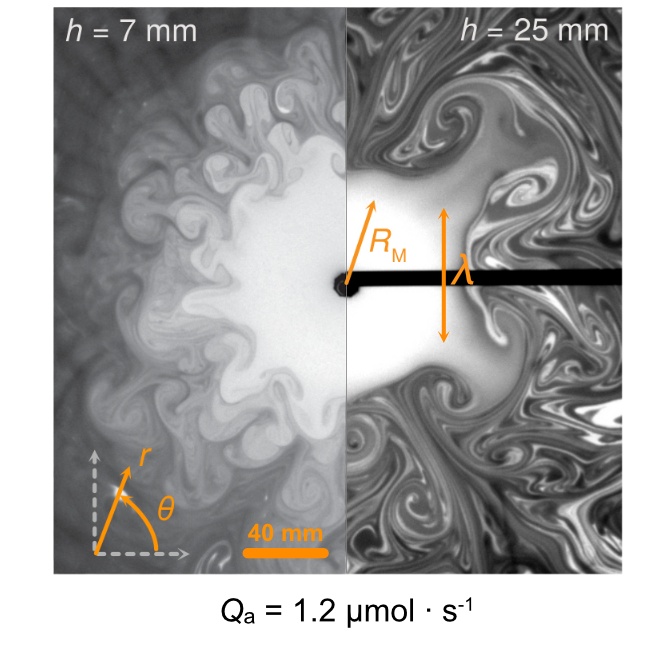
\includegraphics[scale=.55]{./figures/Marangoni_flow_emulsion_Qa1p2mumolL_h7mm_h25mm.png}
    \captionof{figure}{ Deux photos superposées de l'écoulement de Marangoni. La première avec une épaisseur d'eau $h=7~\rm mm$ et un débit molaire $Q_{\rm a} = 1.2~\rm\upmu mol\cdot s^{-1}$ et la seconde avec $h=25~\rm mm$ et $Q_{\rm a} =1.2~\rm \upmu mol\cdot s^{-1}$.}
    \label{fig:EcoulementEpaisseurEau}
  \end{minipage}\hspace{.5cm}
  \begin{minipage}[c]{0.55\linewidth}
    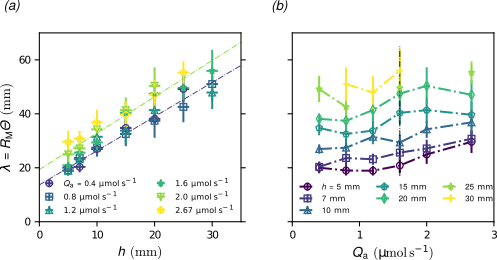
\includegraphics[scale=.65]{./figures/lambda_dossierdidactique.png}
    \captionof{figure}{ (a) Dépendance de la distance moyenne $\lambda$ séparant deux paires de tourbillons sur la couche d'eau d'épaisseur $h$ Les lignes en pointillés représentent une régression linéaire de la forme: $\lambda = Ah+\lambda_0$. (b) Dépendance de la distance moyenne $\lambda$ en fonction du débit molaire $Q_{\rm a}$ (la ligne en pointillé est un guide pour le regard).}
    \label{fig:ThetaLambda}
  \end{minipage}\smallskip

La figure \ref{fig:EcoulementEpaisseurEau} montre la différence de structure de l'écoulement lorsque la hauteur de la couche d'eau passe de $h=\SI{7}{mm}$ à $h=\SI{25}{mm}$ à $Q_{\rm a}$ constant. La taille de l'écoulement de Marangoni reste constante $R_{\rm M} = \SI{50}{mm}$, mais la taille et le nombre de tourbillons ont changé. Dans le cas $h=\SI{7}{mm}$, on compte sur un demi-cercle $6$ paires de tourbillons émis simultanément, de taille $d=\SI{20}{mm}$ et séparées les unes des autres d'une distance $\lambda = \SI{15}{mm}$. Tandis qu'à $h=\SI{25}{mm}$, on en compte $2$ de plus grande taille $d=\SI{40}{mm}$, séparées de $\lambda = \SI{50}{mm}$. Sur la figure \ref{fig:ThetaLambda} j'ai reporté les mesures de $\lambda$ en fonction de l'épaisseur d'eau. On observe que la distance moyenne $\lambda$ séparant deux paires de tourbillons est proportionnelle à $h$ pour les différents débits  $Q_{\rm a}$. Au-delà de $h_{\rm max} = 40~\rm mm$ j'ai observé la disparition de l'émission de tourbillons. En fonction du débit $Q_{\rm a}$, la distance  $\lambda$ reste constante.\medskip

 Mon travail a permis de montrer que la génération des tourbillons dépend de l'épaisseur d'eau  et donc que la structure des tourbillons est liée à un écoulement qui a lieu sous la surface.\medskip

% Nous pouvons distinguer deux familles de courbes sur la figure \ref{fig:ThetaLambda}\textcolor{blue}{(b)}. Les deux familles se distinguent au passage d'un débit critique $Q_{\rm a,c}$ vers $1.2~\rm \upmu mol\cdot s^{-1}$.  Néanmoins, il faut remarquer que le plateau semble changer de valeur au passage de la valeur critique $Q_{a,c}=\SI{1.2}{\upmu mol\cdot s^{-1}}$. Cet effet est lié à un élargissement de la zone de dépôt du tensioactif à fort débit, par conséquent $R_M$ augmente et $\lambda$ aussi. C'est ce qui explique la deuxième famille de courbes pour $\lambda =f(h)$.

\noindent\underline{\textbf{Écoulement sous la surface et mécanisme de génération tourbillonaire}}\medskip

Les résultats précédents nous suggèrent que le mécanisme responsable de la génération de tourbillons à la surface de l'eau résulte d'effets se produisant sous la surface. On étudie l'écoulement sous la surface grâce à la méthode de PIV. Après enregistrement d'un film on obtient en superposant les images la figure \ref{fig:ZprojectImageJ}. On observe que l'écoulement ressemble à un tourbillon qui occupe toute l'épaisseur de la couche liquide. À partir de film, en comparant deux images successives au cours du temps on peut calculer le champ de vitesse $\vv{v} = v_{x}\vv{e_{x}}+v_{z}\vv{e_z} \label{eq:ChampVitesse}$ et la vorticité qui s'écrit comme le rotationnel du champ de vitesse $\vv{v}$: $\vv{\omega}= \vv{\text{rot}}\vv{v}=\vv{\nabla}\wedge\vv{v} \label{eq:VecteurTourbillon}$ présentés sur la figure \ref{fig:PIV}. Les résultats que j'ai obtenu de ces observations m'ont permis d'en déduire un mécanisme possible pour la génération de la vorticité au voisinage de l'écoulement de Marangoni. Ce mécanisme a lieu en plusieurs étapes.\medskip


% \noindent\begin{minipage}[c]{0.45\linewidth}
%   \centering
%   %\resizebox{.7\textwidth}{!}{\input{SchemaEnroulement.pdf_tex}}
%   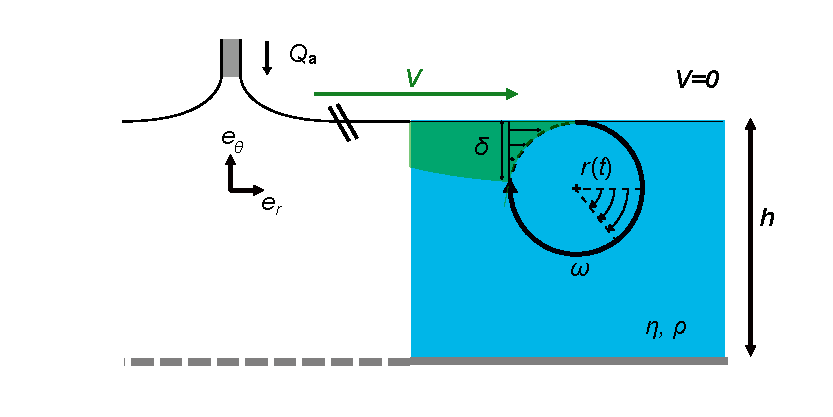
\includegraphics[width=1\textwidth]{Schema_enroulement_v2.pdf}
%   \captionof{figure}{Schéma qui résume la situation}
% \end{minipage}\hspace{.5cm}
% \begin{minipage}[c]{0.45\linewidth}
% 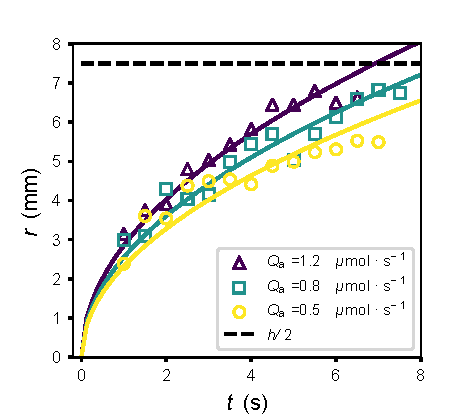
\includegraphics[width=1\textwidth]{Rayon_vs_modele.pdf}
% \captionof{figure}{croissance du tourbillon pour différents débit molaires $Q_{\rm a}$ à une épaisseur d'eau fixée}
% \label{fig:Rayon}
% \end{minipage}\smallskip
1. L'écoulement de Marangoni stationnaire cisaille la surface de l'eau sur une distance qui est le rayon de l'écoulement $R_M$ avec une vitesse maximale $v_M$ dont la quantité de mouvement diffuse sur une épaisseur de liquide $\delta$. On sait qu'un écoulement de cisaillement génère de la vorticité, celle-ci est contenue dans la couche limite et transportée jusqu'à ce que l'écoulement s'arrête.\medskip 

2. La fin de l'écoulement de Marangoni et la modification du profil de vitesse entraîne l'enroulement de la couche limite sous la surface. Ceci fait penser au théorême de Kelvin qui nous dit qu'un écoulement parfait, incompressible et stationnaire conserve la circulation. Par conséquent si un écoulement présente une vorticité non nulle au départ il doit la conserver. Lorsque le transport de la vorticité dans la couche limite s'arrête. Par conservation du moment angulaire les particules fluides se mettent à tourner sur elle-même.\medskip

3. Cet enroulement est toujours en contact avec la couche de limite de vorticité $\delta$ qui l'approvisionne en masse de liquide. En faisant l'hypothèse que le liquide qui entre dans l'enroulement n'en sort pas. C'est ce que j'observe expérimentalement, toute la quantité de mouvement reste dans le vortex. On peut calculer par conservation de la quantité de matière une croissance de l'enroulement $r(t)=\delta\sqrt{1+vt/(2\pi\delta)}$. La croissance d'un tourbillon en $\sqrt{t}$ est typique de la diffusion de la quantité de mouvement du vortex.\medskip

4. La croissance du vortex est uniquement limitée par la présence du fond de la couche d'eau. Lorsque le tourbillon \og{}voit\fg{} le fond de la cuve il cisaille liquide entre le fond et lui-mème ce qui crée une deuxième couche limite de vorticité au voisinage de la paroi immobile. Si le premier vortex est suffisamment fort, il peut entraîner la couche limite de vorticité autour de lui et créer un second vortex qui tourne alors dans le sens opposé.\medskip 

5. L'interaction entre les deux vortex est instable et a plusieurs conséquences. On peut observer des oscillations suivant l'axe de rotation du vortex primaire jusqu'à sa brisure en paire de vortex dont l'axe de rotation est perpendiculaire au premier vortex. C'est ce que l'on appelle dans la littérature l'instabilité des vortex en effet de sol [Harris 2012].%\cite{Harris2012}.

\begin{SCfigure}[0.5][ht]
  \centering
  %\resizebox{.7\textwidth}{!}{\input{SchemaEnroulement.pdf_tex}}
  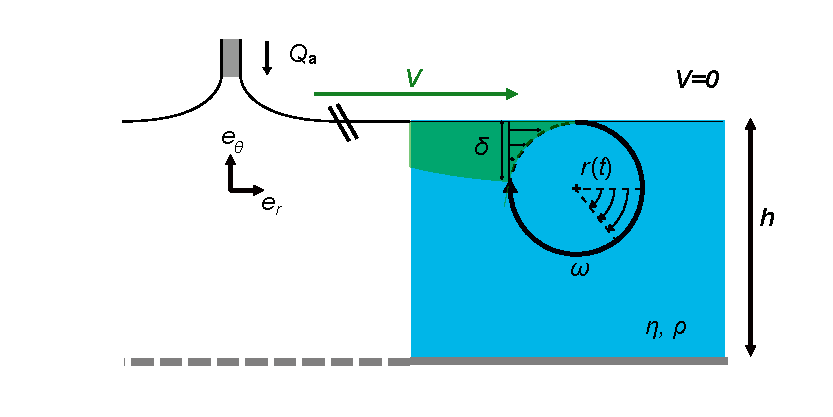
\includegraphics[width=.5\linewidth]{Schema_enroulement_v2.pdf}
  \caption{Schéma de l'écoulement de Marangoni couplé au tourbillon sous la surface de l'eau}
\end{SCfigure}

\begin{figure}[!ht]
\noindent\begin{minipage}[c]{0.48\linewidth}
  \resizebox{1\textwidth}{!}{\input{./figures/Enroulement_stack_v2.pdf_tex}}
  \captionof{figure}{Enroulement sous la surface par la PIV. Projection de $100$ images d'un film de PIV dans les conditions expérimentales suivantes: $h=15~\rm mm$ et $Q_a=0.53~\rm \upmu mol\cdot s^{-1}$. }
  \label{fig:ZprojectImageJ}
\end{minipage}\hfill
\begin{minipage}[c]{0.48\linewidth}
  \centering
  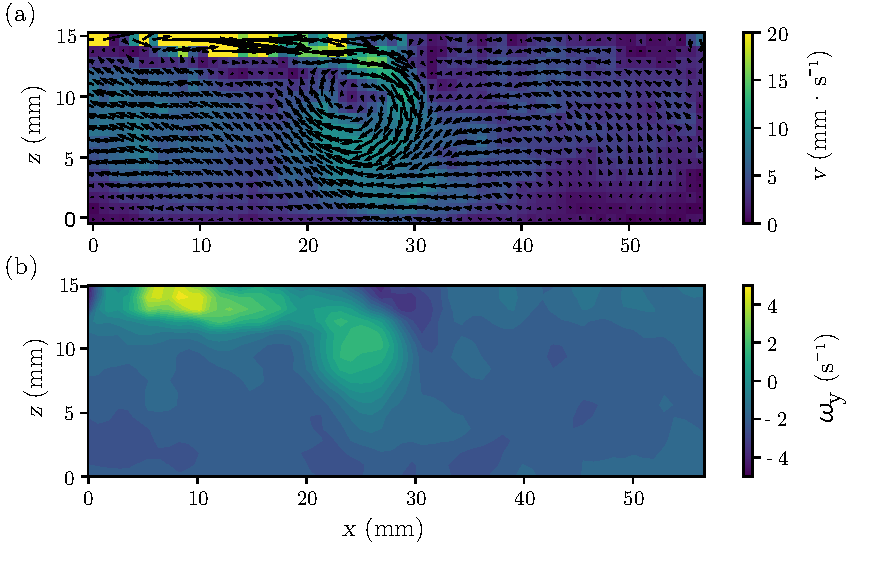
\includegraphics[width=.9\linewidth]{./figures/rolling_vortex_velocity_vorticity_v2.pdf}
  \captionof{figure}{(a) Mesure du champ de vitesse.(b) Mesure du champ de vorticité. Pour $h=15~\rm mm$ et $Q_{\rm a}=1.2~\rm \upmu mol\cdot s^{-1}$.   ($\omega_y$).}\label{fig:PIV}
\end{minipage}\medskip
\end{figure}







% \begin{wrapfigure}{r}{.5\textwidth}
%   \centering
%   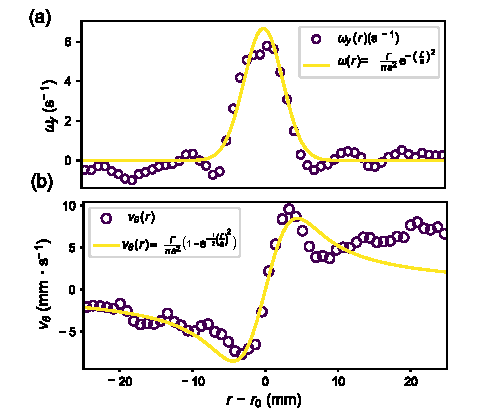
\includegraphics[width=.5\textwidth]{./figures/Vorticityprofile_v2.pdf}
%   \caption{(a) Profil de vorticité, $\Gamma = 267~\rm mm^2\cdot s^{-1}$ et la demi-largeur de la gaussienne $a=3.94~\rm mm$.  (b) Profil de la vitesse azimutale du vortex. Ces profils sont mesurés pour une épaisseur d'eau de $h=15~\rm mm$ et un débit molaire d'injection $Q_{\rm a} = 1.2~\rm \upmu mol\cdot s^{-1}$.}
%   \label{fig:VorticityAzimuthalVelocity}
% \end{wrapfigure}

% Sur la figure \ref{fig:ZprojectImageJ}, nous pouvons voir que la vitesse proche de la surface est $v_{\rm max} = \SI{20}{mm\cdot s^{-1}}$, tandis que dans le tourbillon la vitesse diminue jusqu'à $v_{\rm min} = \SI{10}{mm\cdot s^{-1}}$. Dans le reste de la fenêtre de PIV, l'écoulement est quasi-inexistant, la mesure du champ de vorticité montre qu'elle est centrée sur le c\oe ur du tourbillon où le maximum de $\omega_{\rm y}$ est atteint. La représentation en niveaux de vorticité avec la fonction \textit{contourf} de Matlab permet de visualiser les différentes régions sur la carte de vorticité. Nous voyons ainsi apparaître la couche limite de vorticité qui vient s'enrouler pour former le vortex. Nous remarquons parfois une petite zone de vorticité négative entre le début de l'enroulement et la surface du liquide. À partir de ce type de champ de vorticité, nous pouvons extraire le profil de vorticité de l'enroulement. 

% Le profil de vorticité de l'enroulement est de type gaussien comme le montre la figure \ref{fig:VorticityAzimuthalVelocity}.\medskip

% Ce type de profiles rappelle certaines familles de tourbillons bien connus comme les vortex de Burgers et Rott\cite{Burgers1948, Rott1958} ou les vortex de Lamb-Oseen \cite{Saffman1995} dont la vitesse orthoradiale du tourbillon $v_{\theta}$ et la vorticité qui en découle ont des profils de type Gaussien. Le tourbillon de Burgers existe grâce à l'équilibre entre le cisaillement qui concentre la vorticité en un point de l'espace et sa dissipation par viscosité qui a pour effet de l'étendre dans l'espace. Le tourbillon de Lamb-Oseen est uniquement soumis à la dissipation visqueuse et son rayon augmente en suivant la loi $a=(\sigma t)^{1/2}$ alors que $\Gamma$ reste constant. 

% \begin{equation}
%   v_{\theta}(r)= \dfrac{\Gamma}{2\pi r}\left(1-{\rm e}^{-\left(\dfrac{r^2}{2a^2}\right)}\right);\hspace{2cm} \omega(r) = \frac{\Gamma}{\pi a^2}{\rm e}^{-\left(\dfrac{r}{a}\right)^2} \label{eq:GaussianVorticity}.
% þ\end{equation}

% Ces tourbillons sont caractérisés par $\Gamma$ la circulation du vortex et $a$ le rayon du tourbillon. Dans le cas des tourbillons de Burgers $a = (\nu/\sigma)^{1/2}$ où $\nu$ est la viscosité cinématique et $\sigma$ le taux de cisaillement de l'écoulement environnant le vortex ($\vv{v_{\sigma}} = (-\frac{1}{2}\sigma x,~-\frac{1}{2}\sigma y, \sigma z)$).  Nous avons tracé sur la figure \ref{fig:VorticityAzimuthalVelocity}\textcolor{blue}{(b)} le profil de vitesse azimutale en fonction de la position $r$ par rapport au centre du tourbillon ainsi que le profil de vorticité.\bigskip

% \begin{wrapfigure}{r}{.5\textwidth}
%   \centering
%   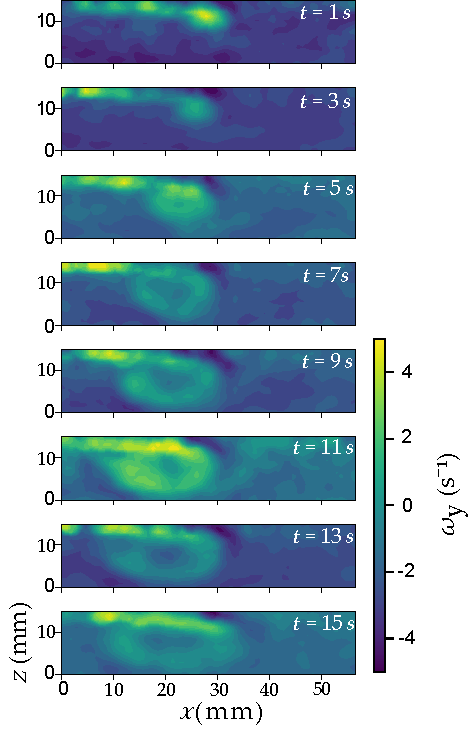
\includegraphics{./figures/Diaporama_rolling_vortex_velocity_vorticity_v4.pdf}
%   \caption{ Diaporama du champ de vorticité sous la surface pendant 8 secondes. Paramètres expérimentaux: $h=15~\rm mm$ et $Q_{\rm a}=1.2~\rm \upmu mol\cdot s^{-1}$.}
%   \label{fig:Diaporama}
% \end{wrapfigure}

% Sur la figure \ref{fig:Diaporama} nous avons tracé un diaporama du champ de vorticité du tourbillon entre sa naissance et sa déstabilisation. La naissance du tourbillon a lieu à $t=t_0$ qui correspond à l'épaisseur de la couche limite lorsque le tourbillon commence à s'enrouler. Le tourbillon croît au cours du temps. Il conserve un profil gaussien jusqu'à atteindre un diamètre de $80\%$ de la hauteur d'eau dans la cuve $h$. À partir de cet instant, le profil de vorticité s'aplatit et se creuse jusqu'à présenter une vorticité nulle au centre de l'enroulement et une vorticité positive tout autour. La déstabilisation du vortex peut avoir lieu même avant, parfois le c\oe ur du tourbillon se déplace vers le fond ce qui le déstabilise plus rapidement. Comme le vortex est piégé entre la surface de l'eau et le fond de la cuve, lorsqu'il interagit avec le fond, il s'étale horizontalement jusqu'à se \og briser \fg pour recommencer à s'enrouler près de la surface et ainsi de suite. L'ouverture du c\oe ur du vortex s'accompagne du cisaillement du liquide piégé entre la paroi du fond et le vortex. Cela entraîne la génération d'une deuxième couche limite près de la paroi que nous pouvons voir sur le diaporama à partir de $t=3~\rm s$ (voir figure \ref{fig:Diaporama}) par un signal de vorticité négative à l'arrière du tourbillon au voisinage du fond. Nous définissons un rayon du tourbillon $r(t)$ que nous mesurons à partir des profils de vorticité gaussiens, lorsque $\omega_{\rm y}=0$. Nous utilisons ce critère pour mesurer la croissance du tourbillon au cours du temps jusqu'à ce qu'il perde le profil de vorticité gaussien où le rayon du tourbillon ne peut plus être correctement défini car il ne s'agit plus d'une rotation solide comme nous pouvons le voir sur la figure \ref{fig:Diaporama} à partir de $t=7~\rm s$. La taille du tourbillon croît (voir figure \ref{fig:RayonTourbillon}) avec le temps jusqu'à occuper toute la hauteur de liquide disponible et sa structure change lorsqu'il entre en interaction avec le fond de la cuve.\medskip


% \section{   Modélisation de la croissance du tourbillon}

% Ici, nous proposons un modèle pour décrire la croissance de l'enroulement construit sur nos observations expérimentales tant que le vortex n'interagit pas avec le fond du bassin. Nous considérons un écoulement dans une couche d'eau d'épaisseur $h$, de masse volumique $\rho=10^{3}~\rm kg\cdot m^{-3}$ et de viscosité dynamique $\eta=1\cdot10^{-3}~\rm Pa\cdot s$. L'écoulement de Marangoni cisaille la surface de ce liquide avec une vitesse $v_{\rm M}$ dont la quantité de mouvement diffuse sur épaisseur $\delta$, la couche limite de vorticité. La fin de l'écoulement de Marangoni et la modification du profile de l'écoulement entraîne l'enroulement de la couche limite sous la surface. Cet enroulement est toujours en contact avec la couche limite générée par l'écoulement stationnaire de Marangoni qui l'approvisionne en masse de liquide. Le vortex est caractérisé par son rayon $r$ et sa fréquence angulaire $\omega$. Afin de prédire la croissance de l'enroulement nous écrivons la conservation de la masse, de l'impulsion, et du moment angulaire. À l'état actuel nous négligeons la dissipation visqueuse.

% \begin{figure}[!ht]
%   \centering
%   \resizebox{.7\textwidth}{!}{\input{./figures/SchemaEnroulement.pdf_tex}}
%   \caption{Schéma du vortex}
%   \label{fig:SchemaVortex}
% \end{figure}

% Nous faisons l'hypothèse que la couche limite $\delta$ arrivant sur le vortex est complètement absorbée par ce-dernier et qu'il n'y a pas de liquide sortant de l'enroulement, ce qui est observé grâce aux expériences de PIV. Il en résulte, une accumulation de liquide qui n'est possible que s'il y a une différence de hauteur entre les régions avant et après le vortex. Cette différence de hauteur entraîne une recirculation de liquide ayant lieu entre le fond du bassin et le liquide ce que l'on peut observer sur les mesures de champ de vitesse présentées figure \ref{fig:ChampVitesse}\textcolor{blue}{(a)}. Pour simplifier les calculs, nous considérons une section de l'enroulement donc les équations que nous allons décrire sont définies sur une surface coupant le vortex. Dans ce contexte, nous écrivons la masse surfacique (par unité de longueur) du vortex tel que $m = \pi\rho r^2$. La variation de la masse du vortex avec le temps provient du flux de liquide advecté par l'écoulement surfacique à travers la couche limite $\delta$. Nous écrivons le flux de masse entrant dans le vortex tel que $j_{\rm m}=\rho_{l} v \delta$. La conservation de la masse traduit la variation de la masse au cours du temps $\dot{m}$ en fonction du flux entrant dans le vortex $j_{\rm m}$ et du flux sortant qui est supposé nul d'après les observations expérimentales. Nous aboutissons à l'équation différentielle suivante:
% \begin{equation}
%   \dot{m}= j_{\rm m}\hspace{1cm} \Leftrightarrow\hspace{1cm } 2r\dot{r}= v\delta.\label{eq:diffeqr}
% \end{equation}
% Après intégration, nous obtenons:
% \begin{equation}
%   r^2(t)=\frac{1}{2\pi}\delta v t + C.
% \end{equation}
% La constante d'intégration $C$ correspond à la valeur initiale du rayon du tourbillon. Le rayon initial doit être de l'ordre de l'épaisseur de la couche limite. On suppose donc que :  $r(t=0~\rm s) = \delta$. Ce qui nous amène à l'équation décrivant la croissance du rayon du vortex:

% \begin{equation}
%   r(t)=\delta\sqrt{1+\frac{vt}{2\pi \delta}}.\label{eq:Rayon}
% \end{equation}

% Dans le cas où $\left(2\pi\delta\right)^{-1}vt\gg 1$, nous pouvons évaluer l'ordre de grandeur des vitesses que l'écoulement atteint \textit{i.e.} $v=\mathcal{O}\left(10^{-2}\right)~\rm m\cdot s^{-1}$ et pour la couche limite $\delta=\mathcal{O}\left(10^{-3}\right)~\rm m$. La simplification devient possible lorsque $t\gg 6\cdot 10^{-1}~\rm s$. L'équation se simplifie et s'écrit:
% \begin{equation}
%   r(t)\sim \sqrt{\frac{v\delta t}{2\pi}}.\label{eq:RayonSimplifiee}
% \end{equation}

% $\delta$ peut être déterminé expérimentalement à partir des mesures de PIV, à ceci près que notre champ de vitesse ne possède pas une résolution spatiale verticale très importante. Une fenêtre d'interrogation correspond à $\SI{1}{mm}$. Nous pourrons utiliser ce paramètre pour ajuster l'équation \eqref{eq:Rayon} de $r(t)$ avec les données expérimentales. Sur la figure \ref{fig:RayonTourbillon}\textcolor{blue}{(a)}, nous avons tracé l'évolution du rayon du tourbillon en fonction du temps pour trois débits d'injection $Q_{\rm a}$ à la même hauteur d'eau dans la cuve.  Nous comparons à ces résultats expérimentaux la prédiction de $r(t)$ (équation \eqref{eq:Rayon}). La comparaison entre l'expérience et le modèle présente un bon accord. À partir de l'équation \eqref{eq:Rayon} nous pouvons définir un temps caractéristique $\tau_{\rm b}$ qui est le temps qu'il faut au tourbillon à atteindre le fond du bassin, \textit{i.e.}: $r(\tau_{\rm b})=h/2$. Dans ce cas son équation est la suivante:
% On peut calculer $\delta$ à partir de la vitesse de l'écoulement de surface moyenne $\langle v_{\rm surface}\rangle$ et de la distance sur laquelle s´étend l'écoulement de Marangoni. Pour les lier on utilise l'équation de $\delta$ pour une plaque plane dans un écoulement.
% \begin{equation}
%   \delta(R_{\rm M}) = \sqrt{\frac{\nu R_{\rm M}}{\langle v_{\rm surface} \rangle}}
% \end{equation}

% \begin{equation}
%   \tau_{\rm b} = \frac{\delta}{v}\left(\frac{h^2}{4\delta^2}-1\right)\sim \frac{h^2}{4\delta v}.\label{eq:TimeB}
% \end{equation}

% Nous pouvons remarquer que le rayon $r$ est proportionnel à l'épaisseur de la couche limite. Cette observation permet d'adimensionn l'équation décrivant l'évolution de $\tau_{\rm b}$ (équation \eqref{eq:TimeB}). Pour l'adimensionner, il faut diviser l'équation par $\delta^2$ ce qui donne:

% \begin{equation}
%   \frac{h^2}{2\delta^2}\propto \frac{v\tau_{\rm b}}{\pi \delta}. \label{eq:adim1}
% \end{equation}

% Nous réécrivons cette équation en notant $H^2=h^2(2\delta^2)^{-1}$ et $T=(\pi \delta)^{-1}v\tau$, nous en déduisons l'égalité suivante:

% \begin{equation}
%   T=H^2. \label{eq:adimensionne}
% \end{equation}

% Sur la figure \ref{fig:RayonTourbillon}\textcolor{blue}{(b)}, nous avons tracé le temps adimensionné $T$ que met le tourbillon à interagir avec le fond de la cuve en fonction de l'épaisseur d'eau. Nous voyons sur cette figure que $T$ est proportionnel à $H^{2}$. Les deux hauteurs d'eau pour lesquelles nous avons étudié l'écoulement en volume sont en accord avec la prédiction, nous avons également mesuré le temps d'émission des paires de tourbillons à la surface à partir des visualisations de l'écoulement surfacique. Nous constatons que ces mesures se superposent au temps que met que met le tourbillon à se déstabiliser et à la prédiction donnée par l'équation \eqref{eq:adimensionne}. L'émission des tourbillons à la surface semble correspondre avec la déstabilisation du vortex sous la surface. Nous en déduisons que l'émission des tourbillons à la surface trouve son origine dans la déstabilisation du vortex.

% \begin{figure}[!ht]
%   \centering
%   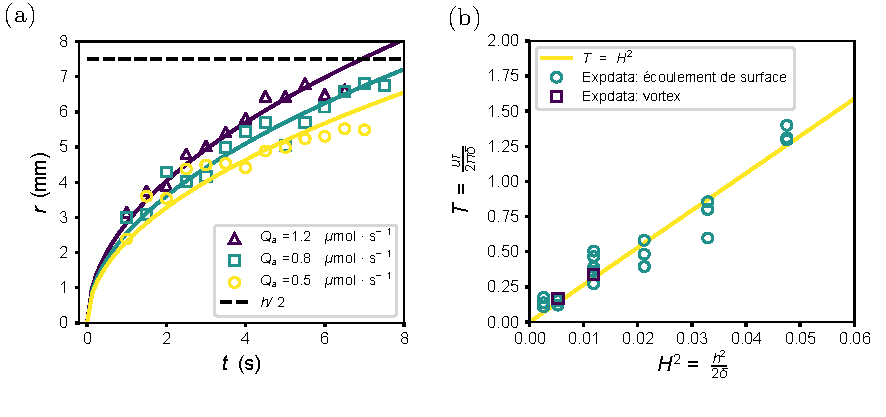
\includegraphics[scale=1]{./figures/Croissance_Rayon_v2.pdf}
%   \caption{(a) - Mesure de la croissance du tourbillon pour $h=15~\rm mm$ et différents débits molaires d'injection $Q_a \in [0.5, 0.8, 1.2]~\rm \upmu mol\cdot s^{-1}$. En ligne solides, nous avons tracé la prédiction pour la croissance du tourbillon (équation \eqref{eq:RayonSimplifiee}) (b) - Corrélation des temps d'émission des tourbillons de la surface avec le temps de de déstabilisation de l'enroulement sous la surface.}
%   \label{fig:RayonTourbillon}
% \end{figure}
% 
% Bien que simple, ce modèle nous permet d'obtenir plusieurs informations sur notre système et sur l'origine de l'instabilité que nous observons en surface. La mesure du temps d'émission des tourbillons et du temps que met le tourbillon à se déstabiliser montre que les deux phénomènes sont étroitement liés. De plus, l'évolution du rayon du tourbillon nous donne des informations sur la nature de l'interface à l'extérieur de l'écoulement de Marangoni, c'est l'objet de la section suivante.
% 
% 
% \begin{Programme}{BO: deuxième année PC - Conservation de la quantité de matière}
	% \begin{enumerate}
		% \item vecteur densité de flux de particules;
		% \item Bilan de quantité de matière entrant dans un volume de contrôle;
    % \item Flux de masse
		% \item échelle caractéristique de diffusion.
	% \end{enumerate}
% 
	% On peut proposer un exercice mêlant vorticité et taille du tourbillon que l'on peut estimer grâce à la conservation de la masse.
% \end{Programme}
% 
% \subsubsection{Conclusion}
% 
% Dire que c'est similaire des écoulement d'enroulement de couches limites que l'on trouve dans d'autres systèmes. Et que ça donne des informations sur l'environnmenent du tourbillon. Nous en déduisons que la croissance de l'enroulement dépend fortement de son environnement qui peut imposer des conditions différentes au voisinage du tourbillon. La condition de non-glissement qu'impose la présence d'une surface rigide au voisinage du vortex entraîne l'apparition de vorticité secondaire qui perturbe la croissance du vortex primaire. La loi qui ressort de notre étude correspond à la situation que Sattari \textit{et al} décrivent. Ceci indique que la surface à côté de laquelle notre enroulement apparaît, est une surface qui agit comme une surface libre où la quantité de mouvement est dissipée par viscosité. Bien que nous puissions distinguer la génération de vorticité négative au voisinage de la surface \ref{fig:ChampVitesse} elle est faible et ne semble pas perturber la croissance de l'enroulement. De plus nous avons vu que si la surface de l'eau est contaminée par des molécules tensioactives, l'accumulation des molécules peut former un film qui impose des conditions de vitesse nulle à la surface (voir \ref{section:soluto-capillaire}). Le fait que la surface agit comme une surface libre est intéressant car ça signifie que si contamination il y a, elle est faible et cela corrobore les observations faites par \cite{Leroux2016}. Pour conclure, nous avons montré à travers plusieurs techniques que la génération des tourbillons à la surface près de l'écoulement de Marangoni trouve son origine dans la déstabilisation d'un vortex toroïdal en effet de sol sous la surface de l'eau.\bigskip 
% 
% Grâce à une méthode de visualisation de l'écoulement à la surface, nous avons pu caractériser la génération des tourbillons. Cette instabilité se caractérise par une longueur d'onde $\lambda$ qui correspond à la distance séparant des émissions simultanées de tourbillons. Nous avons montré que $\lambda$  est proportionnelle à l'épaisseur de la couche d'eau dans la cuve. Par conséquent à $h$ fixé, si le débit d'injection augmente et la taille de l'écoulement par la même occasion, le nombre de tourbillons générés augmente.\bigskip
    % 
% La visualisation de l'écoulement sous la surface par la PIV a montré que l'écoulement de Marangoni génère une couche limite de vorticité. Celle-ci s'enroule lorsque l'écoulement de Marangoni atteint sa distance maximale. L'enroulement génère un vortex toroïdal sous la surface qui en interagissant avec la paroi du fond génère de la vorticité secondaire. Par similarité avec les vortex en effets de sol, nous attribuons la déstabilisation du système à une instabilité de Crow de courte longueur d'onde. Cette instabilité s'accompagne de motifs de paires de tourbillons émis perpendiculaire à la vorticité du vortex primaire.\bigskip
% 
% Nos expériences nous donnent des indications sur la nature de l'interface hors de l'écoulement de Marangoni. La croissance du tourbillon en racine du temps suggère que la surface de l'eau se comporte comme une surface libre, c'est à dire sans la présence de contaminant, ce qui est conforté par l'absence de ridge de Reynolds à la surface de l'eau. Le fait que la surface de l'eau soit peu contaminée offre la possibilité à la vorticité générée en volume de se reconnecter à la surface. Par conséquent, nous attribuons la génération de vorticité à la surface à la reconnexion de la vorticité du volume à la surface.\bigskip
% 
% L'écoulement de Marangoni soluto-capillaire offre la possibilité d'étudier la génération et la dynamique de tourbillons près d'une paroi ou d'une surface déformable. En particulier, grâce à sa stabilité et sa reproductibilité.
% 

% 
\section{Bateaux de Marangoni}


Pendant ma thèse je me suis intéressé à un autre aspect lié à l'effet Marangoni : la propulsion de bateaux de Marangoni. Ce sujet a fait l'objet de nombreuses études dans la littérature, notamment en médecine on sait réaliser des micro-robots pour amener les médicaments à des cibles précises dans l'organisme. Ces objets permettent également de comprendre comment certains insectes sont capables de se propulser à la surface de l'eau à des vitesse de l'ordre du demi-mètre par seconde. 


% 
% \noindent \textbf{Effet de la physicochimie sur la propulsion des bateaux de Marangoni:}\bigskip
% 
% Dans un second temps, nous nous sommes intéressés à la propulsion de petits objets par effet Marangoni. 
% 
% \subsection{Propulsion de bateaux de Marangoni}
% 
% Dans la nature, nous pouvons observer des insectes qui profitent de la tension de surface pour survivre, se déplacer et se nourrir à la surface de l'eau \cite{Milne1978}. Parmi les plus connus et étudiés citons les \textit{gerris}, ce sont des araignées d'eau qui mesurent environ $\SI{5}{mm}$. Elles peuvent se déplacer aisément à la surface des mares comme illustré sur la figure \ref{fig:insectes}\textcolor{blue}{(a)}. Elles sont capables de rester sur la surface de l'eau grâce aux poils présents sur leurs pattes qui leur confèrent de l'hydrophobicité et leur permet de s'appuyer sur l'eau sans couler \cite{Yang2019, Benzaquen2018}. De cette façon, les \textit{gerris} peuvent se déplacer en ramant avec leurs longues pattes.\bigskip 
% Certains insectes sont capables de se propulser à de très grandes vitesses à la surface de l'eau grâce à l'effet Marangoni  \cite{Hu2006}. La première observation de la propulsion d'un insecte par effet Marangoni a été relevée par Billard et Bruyant en 1905: un \textit{stenus} (insecte terrestre) lâché sur une mare, est capable de rejoindre la terre ferme rapidement sans aide extérieure, sans nager ou ramer. Ils parviennent à s'auto-propulser en lâchant des tensioactifs sur l'eau.\bigskip
% 
% Ce phénomène a été observé chez des insectes de la famille des coléoptères, ou d'autres insectes semi-aquatiques comme la \textit{microvelia}. C'est un insecte qui mesure $2~\rm mm$ de long qui est capable de se propulser à des vitesses de l'ordre de $v_{\rm prop}\approx 20~\rm cm\cdot s^{-1}$. Cet insecte est visible sur la figure \ref{fig:Microvelia}. L'insecte vient de se propulser sur de l'eau et la trajectoire est visible, car les impuretés sur l'eau ont été écartées lors de son passage laissant apparaître une eau plus claire et plus propre.\bigskip
% \begin{wrapfigure}{r}{.5\textwidth}
	% \centering
	% 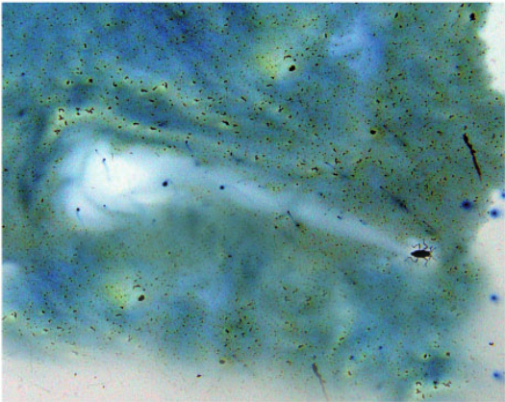
\includegraphics[width=.3\textwidth]{./figures/Microvelia.pdf}
	% \caption{Auto-propulsion de la \textit{Microvelia} sur de l'eau. La traînée du parcours de l'insecte est visible, car en relargant les tensioactifs elle a écarté les impuretés à la surface de l'eau. (Photo prise par Andersen en 1982)}
	% \label{fig:Microvelia}
  % \end{wrapfigure}
% 
% \begin{figure}[!ht]
% 	\centering
% 	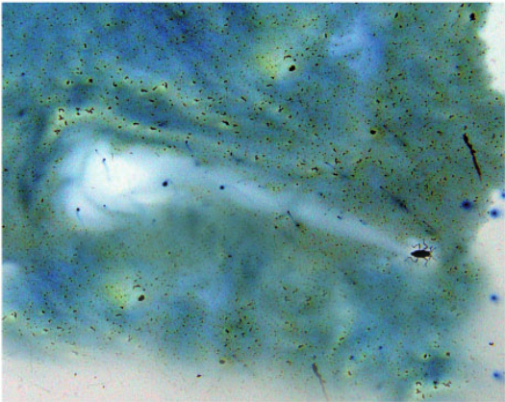
\includegraphics{./figures/Microvelia.pdf}
% 	\caption{Auto-propulsion de la \textit{Microvelia} sur de l'eau. La traînée du parcours de l'insecte est visible, car en relargant les tensioactifs elle a écarté les impuretés à la surface de l'eau. (Photo prise par Andersen en 1982)}
% 	\label{fig:Microvelia}
%   \end{figure}
%   % 
  % Le mécanisme utilisé par ces insectes a inspiré les chercheurs pour créer des systèmes capables de s'auto-propulser à la surface d'un liquide par effet Marangoni. Burton \textit{et al} \cite{Burton2014} ont montré qu'ils pouvaient propulser des petits objets appelés les bateaux de Marangoni à des vitesses similiares à celles de la \textit{microvelia}. Le bateau consiste en un morceau de plastique découpé sur lequel ils accrochent un petit bloc de tensioactif à base d'éthanol. Nous allons voir dans les sections suivantes qu'une large gamme de systèmes très différents capables de s'auto-propulser ont vu le jour. En particulier des billes liquides, des gouttes et des bateaux de camphre. Ces systèmes présentent des dynamiques variées dépendant à la fois du volume de la goutte, de la géométrie du bateau, de la concentration en tensioactifs et de leur environnement. 
% 
  % Nous avons montré dans la première partie de cette thèse que l'effet Marangoni peut être déclenché par des tensioactifs hydrosolubles. Il est donc aussi possible de propulser des bateaux de Marangoni à l'aide de tensio-actifs hydrosolubles. L'usage de tensioactifs solubles ajoute un degré de complexité au problème car ces tensio-actifs solubles restent à la surface du liquide ou dans le volume pendant le voyage du bateau.\bigskip
% 
\subsection{Principe}



Lorsque le bateau de Marangoni se déplace à la surface de l'eau les tensioactifs contenus sur le bateau sont libérés sur la surface du liquide et s'étalent. 

\begin{wrapfigure}{r}{.5\textwidth}
  \centering
  \resizebox{.5\textwidth}{!}{\input{./figures/sketchsoapboat.pdf_tex}}
  \caption{Schéma des bateaux de Marangoni solutal}
  \label{fig:sketchsoapboat}
\end{wrapfigure}


\noindent L'étalement des tensioactifs solubles sur le liquide est une situation hors-équilibre, car les tensioactifs peuvent désorber et s'adsorber à l'interface en plus d'être transportés par l'écoulement de Marangoni. Ces phénomènes se traduisent par la relation entre la concentration surfacique des tensioactifs $\Gamma(r,t)$ et la concentration en volume des tensioactifs $c(r,z,t)$ dont dépend la tension interfaciale $\gamma(r,t)$ à chaque instant pendant le mouvement du bateau. Alors que les tensioactifs sont libérés, le gradient de tension de surface diminue au cours du temps jusqu'à ne plus pouvoir générer de propulsion. La vitesse du bateau diminue avec la diminution de la différence de tension de surface jusqu'à son arrêt complet lorsque $\Delta\gamma =0$ entre la proue et la poupe du bateau (voir figure \ref{fig:sketchsoapboat}).

\subsection{Dispositif expérimental}

Le dispositif expérimental construit pour étudier la propulsion des bateaux par effet Marangoni est composé d'une cuve en forme de fleur (voir figure \ref{fig:cuve}) posée sur une plateforme permettant d'en assurer l'horizontalité. Un panneau de leds permet d'éclairer le tout par en-dessous. Les expériences sont enregistrées par-dessus avec une caméra (Imagine Source DMK $\rm 23U445$) à une fréquence de $10$ images par secondes pour suivre la trajectoire du bateau. La forme particulière de la cuve est primordiale, elle permet d'éviter que le bateau se coince contre les bords. Lorsqu'il rentre en contact avec la paroi il est redirigé vers le centre grâce à la forme incurvée des parois, ceci permet d'éviter un contact prolongé avec les bords de la cuve. Le bateau est composé de deux parties. La première est le flotteur, il s'agit d'une feuille de plastique transparente découpée en forme de hors-bord. La longueur du bateau est $L=2~\rm cm$ et de largeur $W = 1.5~\rm cm$ comme illustré sur la figure \ref{fig:schema}. La deuxième partie est le moteur du bateau. Il s'agit d'une languette de papier filtre imbibée de solution de tensioactif de concentration connue. Le moteur est fixé sur le bateau à $l_1 = 1~\rm cm$ de l'arête et déborde sur l'eau sur une distance $l_2 = 2~\rm mm$ et de largeur $w=5~\rm mm$. Pour fixer le moteur au bateau, nous utilisons une pointe de vernis à ongle de couleur sombre. Le vernis permet facilite la détection du bateau pour pointer sa trajectoire. La trajectoire du bateau est reconstituée à l'aide d'un programme python qui permet de détecter les contours du bateau à partir desquels je calcule le barycentre du bateau que l'on suit au cours du temps.\medskip



 J'ai étudié l'influence de la concentration et de la concentration micellaire critique sur la trajectoire et l'évolution de la vitesse du bateau. J'ai mené des expériences pour différents types de tensioactifs (HTAC, TTAB, DoTAB et DeTAB) dont les concentrations micellaire critiques (CMC) sont reportées dans la table \ref{Table:Tablev0} Ces tensioactifs diffèrent de par la la longueur de leur chaîne carbonée et la nature de la tête hydrophile.
 
 \begin{table}[!ht]
  \centering
  \begin{tabular}{llcc}
    \hline \hline
    Tensioactif & Acronyme & CMC ($\rm mmol\cdot L^{-1}$) & $v_{\rm max}$ ($\rm cm\cdot s^{-1}$)\\ \hline \hline
    Hexadecyl Trimethyl Ammonium Chloride &HTAC, $\rm C_{16}TAC$& $1.3$ & $28.1\pm 1.1$ \\
    Tétradécyl Triméthyl Ammonium Bromide &TTAB $\rm C_{14}TAB$ & $3.6$ & $26.5\pm 1.5$\\
    Dodécyl Triméthyl Ammonium Bromide &DoTAB $\rm C_{12}TAB$ & $15.4$ &  $25.2 \pm 1.6$ \\
    Décyl Triméthyl Ammonium Bromide & DeTAB $\rm C_{10}TAB$ & $62.5$ & $22.2\pm 1.1$\\ \hline \hline 
  \end{tabular}
  \caption{Tableau reçapitulatif des tensioactifs utilisés}
  \label{Table:Tablev0}
\end{table}


Je suis donc à même d'enseigner la programmation python au lycée et en filières post-bac. Je l'utilise régulièrement cette année en tant que professeur de physique chimie pour présenter des animations en classe ou bien faire faire aux élèves des mesures, du traitement de données et des modélisations à l'aide du langage python. 

%Pour préparer la solution de tensioactif nous pesons une masse $m_{\rm tensioactif}$ de tensioactif avec une balance de précision. La poudre de tensioactif est ensuite dissoute dans un volume d'eau millipore, généralement de $V=50~\rm mL$ ce qui permet de réaliser plusieurs expériences.
% 
% 
% \begin{figure}[!ht]
%    \centering
%   %  \resizebox{.7\textwidth}{!}{\input{./figures/Dispositif_Exp_Bateau_Marangoni.pdf_tex}}
%    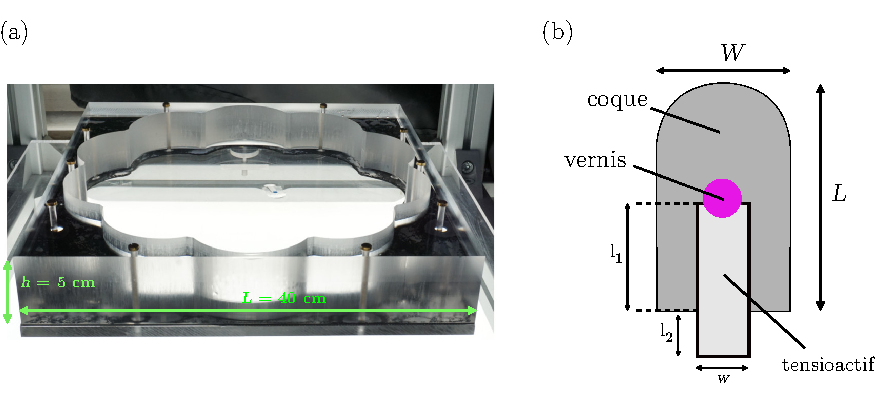
\includegraphics[width = .7\textwidth]{./figures/Dispositif_Exp_Bateau_Marangoni_v2.pdf}
%    \caption{(a) - Photo de la cuve fleurie. La cuve est usinée dans un bloc de plexiglas de hauteur $h=5~\rm cm$ et de $40~\rm cm$ de côté. (b) - Schéma des bateaux de Marangoni.}
%    \label{fig:DispositifExp}
% \end{figure}
% % 


 
\subsubsection{Résultats expérimentaux}

\begin{figure}[ht]
  \centering
  \begin{subfigure}[b]{0.45\textwidth}
      \centering
      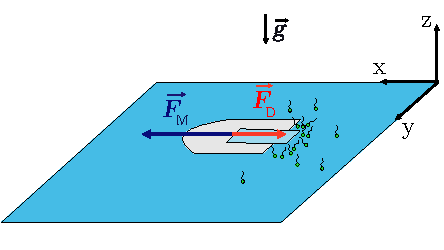
\includegraphics[width=.7\textwidth]{./figures/SchemaModeleBateau.pdf}
	  \caption{Schéma de la modélisation du bateau de Marangoni}
	  \label{fig:schema}
  \end{subfigure}
  \hfill
  \begin{subfigure}[b]{0.45\textwidth}
    \centering
    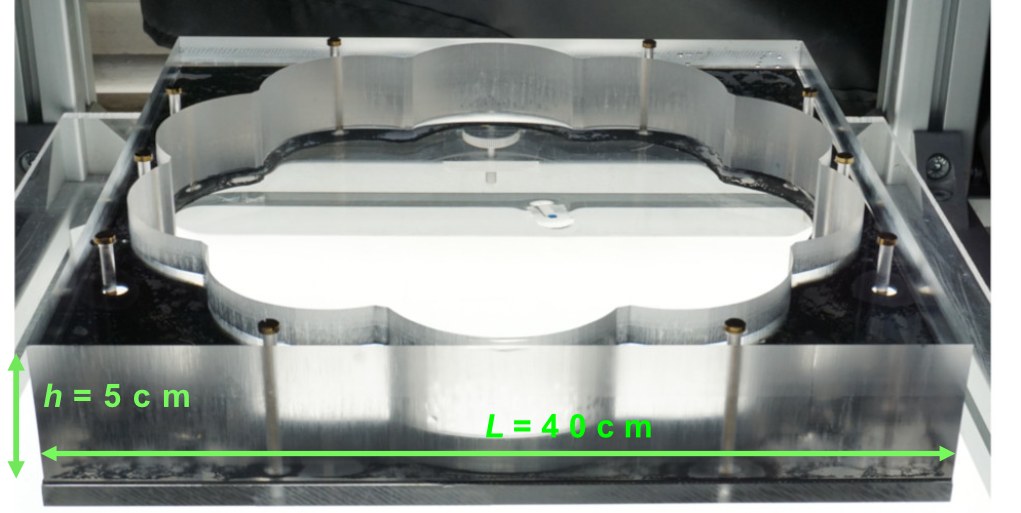
\includegraphics[width=.7\textwidth]{Cuvefleurie.png}
  \caption{Dispositif expérimental, cuve fleurie remplie d'eau pure, avec un bateau posé sur l'eau.}
  \label{fig:cuve}
\end{subfigure}\\
\begin{subfigure}[b]{0.45\textwidth}
  \centering
  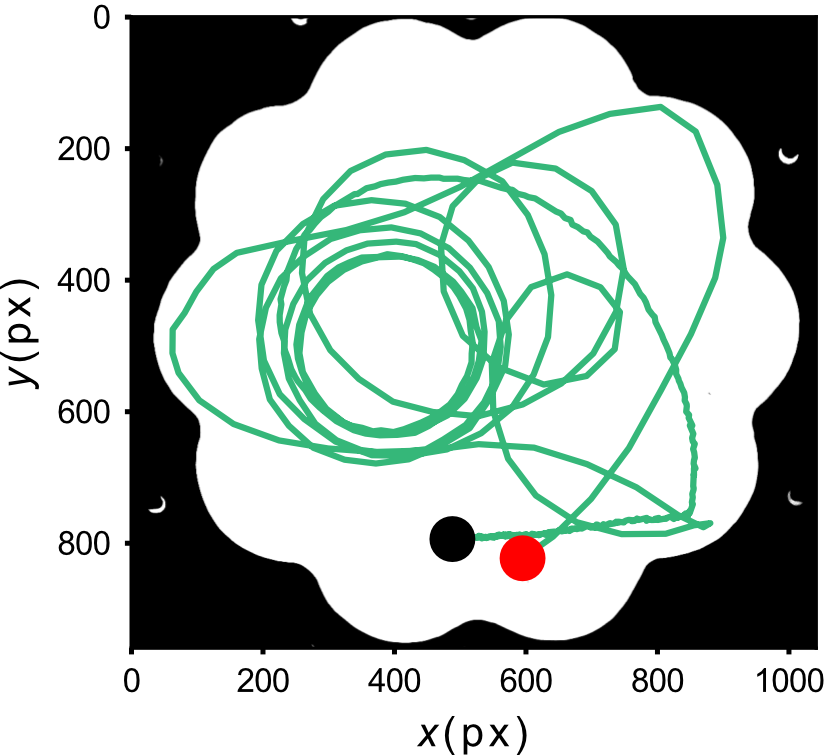
\includegraphics[width=.7\textwidth]{SuiviBateau.png}
\caption{Trajectoire du bateau, le bateau démarre au cercle rouge et s'arrête au cercle noir}
\label{fig:trajectoire}
\end{subfigure}\hfill
\begin{subfigure}[b]{0.45\textwidth}
  \centering
  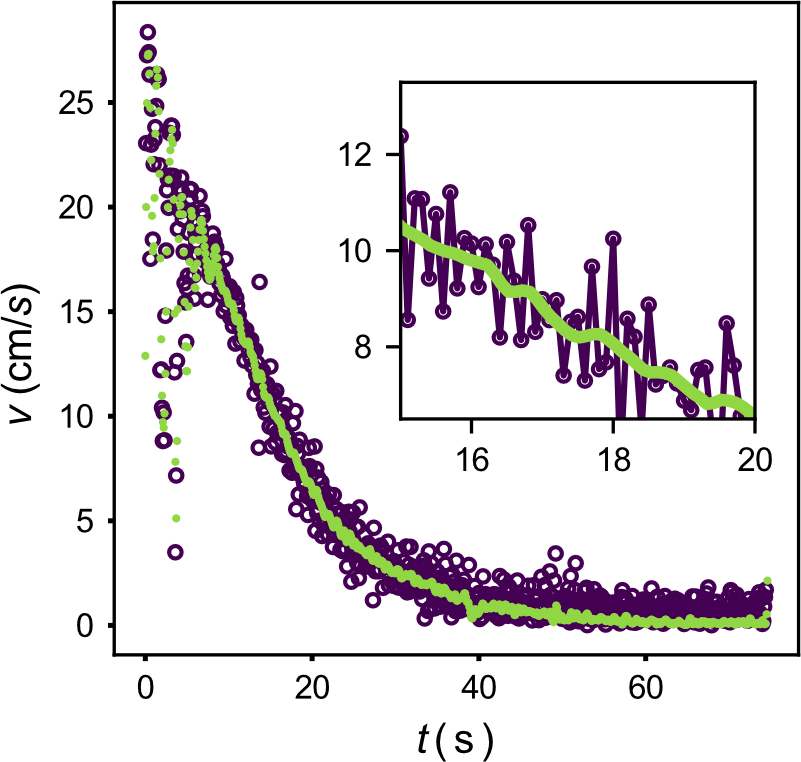
\includegraphics[width=.7\textwidth]{vitesse_t.png}
\caption{Évolution de la vitesse du bateau au cours du temps pour HTAC à $c=0.1~\rm mol\cdot L^{-1}$}
\label{fig:vitesse}
\end{subfigure}\hfill
\caption{Dispositif expérimental et mesure de la vitesse du bateau}
\end{figure}



J'ai étudié l'évolution de la vitesse en fonction de la concentration en tensioactif dans le réservoir. Quel que soit le tensioactif utilisé, l'évolution de la vitesse au cours du temps suit la même allure. Le bateau part avec une vitesse maximale à $t=0~\rm s$ puis décélère sur plusieurs dizaines de secondes ($t_f\approx 60~\rm s$). J'ai reporté les valeurs des vitesses initiales sur le tableau \ref{Table:Tablev0}, pour la même concentration dans le réservoir $c=0.1~\rm mol/L$. On observe que la vitesse initiale du bateau diminue lorsque la CMC augmente. En effet, l'HTAC est le tensioactif le plus efficace et peut propulser les bateaux à de grandes vitesse $v = 28.1~\rm cm\cdot s^{-1}$. Au contraire, le DeTAB est le moins efficace des quatre avec une vitesse de $v=22.2~\rm cm\cdot s^{-1}$. Pour les quatre tensioactifs j'ai tracé l'évolution de la vitesse initiale des bateaux en fonction de la concentration de la solution initiale. Sur la figure  \ref{fig:vitessevo} j'ai reporté la valeur moyenne sur trois réalisations. Nous pouvons remarquer que la vitesse initiale augmente avec la concentration de la solution, d'abord rapidement puis on observe un palier où la vitesse sature. À partir de ces observations, j'ai essayé de proposer un modèle qui tienne compte des paramètres physico-chimiques du système pour comprendre l'influence de la nature du tensioactif ainsi que de sa concentration.



% % 
% \begin{figure}[!ht]
%    \centering
%    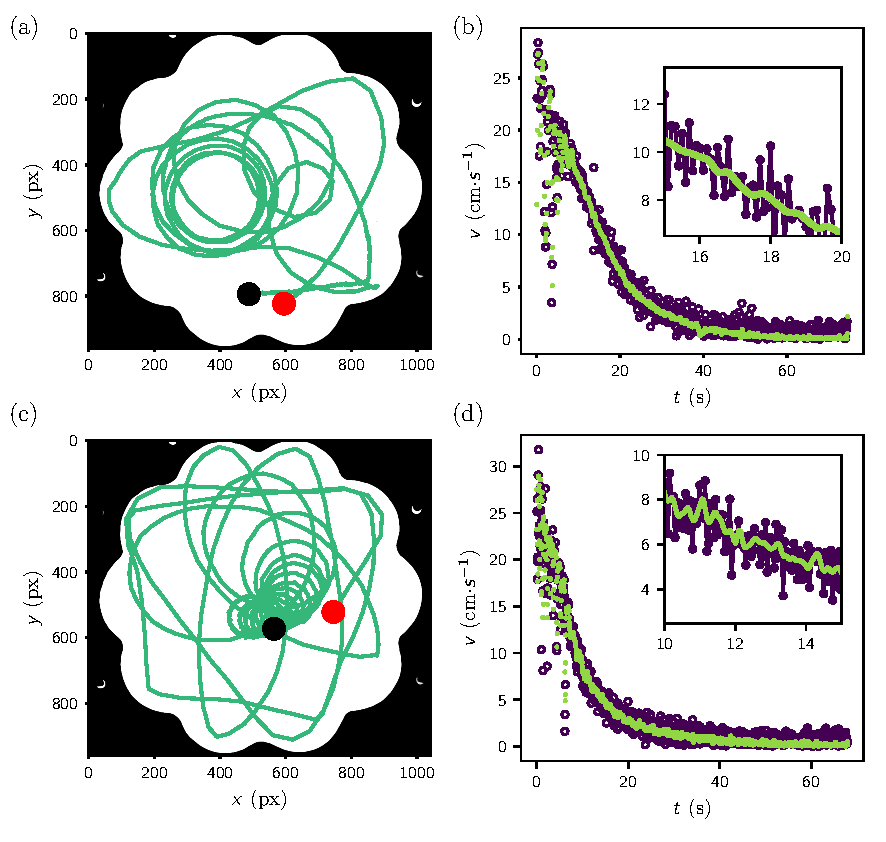
\includegraphics[width=.8\textwidth]{./figures/Trajectoire_velocity_profile_brut_v3.pdf}
%    \caption{Dynamique du bateau. (a) - Trajectoire du bateau (b) - Évolution de la vitesse du bateau au cours du temps pour HTAC à $c=0.1~\rm mol\cdot L^{-1}$. (c, d) - Même chose pour du TTAB à $c=0.4~\rm mol\cdot L^{-1}$ . Paramètres expérimentaux $c$, surfactant: }
%    \label{fig:BateauTrajectoireVitesseBrut}
% \end{figure}

% Nous pouvons voir sur l'image \ref{fig:BateauTrajectoireVitesseBrut}\textcolor{blue}{(a)} que le bateau part avec une trajectoire rectiligne qui devient circulaire par la suite. Lorsque le bateau rencontre les bords, il est doucement redirigé vers le centre de la cuve grâce à la forme de la cuve. Néanmoins, certains chocs peuvent être plus violents, alors sa trajectoire change brusquement de direction et sa vitesse chute drastiquement l'espace d'un instant puis retrouve sa valeur avant le choc. Les chocs entre le bateau et les bords de la cuve ne sont observés que pendant les dix premières secondes de déplacement du bateau lorsque sa trajectoire est encore rectiligne. En effet, pendant que la vitesse du bateau diminue sa trajectoire devient de plus en plus circulaire.\bigskip
% 
% Nous avons vu que Sur \textit{et al} attribuent le type de trajectoire à la vitesse du bateau en forme de disque avec le moteur à l'arrière \cite{Sur2019}. Notamment, ils distinguent deux régimes caractérisés par le nombre de Reynolds. Selon leur étude, la transition a lieu pour des Reynolds compris entre $112<R_e<180$. Leurs bateaux présentent des trajectoires rectilignes lorsque $Re<112$ et des trajectoires circulaires lorsque $R_e>180$. Nous pouvons évaluer le nombre de Reynolds de nos bateaux en considérant qu'ils ont une taille typique de $L=2~\rm cm$ (leur longueur sur suivant leur axe de symétrie), ils se déplacent à une vitesse maximale de l'ordre de $v=25~\rm cm\cdot s^{-1}$ (voir figure \ref{fig:BateauTrajectoireVitesseBrut}) sur de l'eau millipore de viscosité cinématique $\nu = 1.007\cdot 10^{-7}~\rm m^2\cdot s^{-1}$ à $T=20^{\circ} C$. Par conséquent le nombre de Reynolds définit comme $Re=L v/\nu$ est égal à $Re=5000$ donc les trajectoires devraient être circulaires dès le départ si nous faisons référence à \cite{Sur2019}.\bigskip
% 
% Cependant plus le bateau ralentit, plus sa trajectoire est circulaire. Par conséquent nous attribuons les trajectoires circulaires plutôt à des effets de la géométrie du bateau puisque la coque du bateau n'est pas toujours parfaitement symétrique. En effet, le découpage du flotteur est réalisé à la main et est donc soumis à des erreurs de découpage malgré nos précautions. De plus, le moteur peut parfois être positionné de travers ce qui donne au bateau une direction privilégiée à la manière de Su \cite{Su2007}. Les effets de bords ne sont pas à négliger non plus, car le bateau subit des chocs pendant son déplacement et la forme des murs confère au bateau un moment angulaire qui amplifie l'effet de l'asymétrie de la coque. Enfin, lorsque nous réalisons les expériences, nous pouvons observer la génération de vagues autour du bateau. Lorsque le bateau se déplace près du bord celles-ci en rebondissant sur les bords peuvent perturber sa trajectoire.\bigskip
% 
% Sur la figure \ref{fig:BateauTrajectoireVitesseBrut}\textcolor{blue}{(b)} nous avons tracé l'évolution de la vitesse au cours du temps pour une expérience. En \textcolor{cobalt}{bleu marine} la vitesse est calculée par la méthode des différences finies. Le signal fluctue significativement comme nous pouvons le voir sur le zoom que la vitesse. Pour affiner le résultat, nous utilisons un filtre de Savitzky Golay,  qui permet de lisser le signal c'est la courbe en \textcolor{green}{vert}. Le bateau accélère instantanément dès qu'il touche la surface de l'eau et atteint sa vitesse de pointe ($v=25~\rm cm \cdot s^{-1}$) en moins de $t=0.1~\rm s$ qui est la fréquence d'acquisition de notre caméra. Ensuite sa vitesse décroît avec le temps jusqu'à s'arrêter complètement au bout de $70$ secondes. Les résultats qui sont présentés dans la suite sont obtenus par la même méthode et moyennés sur trois expériences menées dans les mêmes conditions expérimentale pour vérifier la reproductibilité.\medskip
% 



% 
% Il faut remarquer que les évènements de chocs apparaissent sur les profils de vitesses moyennes, en particulier sur les graphiques \ref{fig:BateauTrajectoireVitesseBrut}\textcolor{blue}{(b,d)}. Cela montre que les chocs peuvent avoir lieu lorsque le bateau va suffisamment vite sur l'eau. Aux grandes concentrations les profils de vitesses en fonction du temps sont différents, les vitesses atteintes initialement sont plus grande et la décroissance de la vitesse est plus lente. Cette observation semble correspondre aux remarques de de Ender \textit{et al} \cite{Ender2021}. ils avaient remarqué que plus la vitesse du bateau est grande moins le gradient de concentration et de tension de surface faiblit vite. Nous voyons aussi des phénomènes curieux pendant la décroissance avec l'apparition de paliers.\medskip
  % \begin{figure}[!ht]--
  %   \centering
  %   %\includegraphics[scale=.5]{./figures/chap3/Deceleration_bateau_Marangoni.pdf}
  %   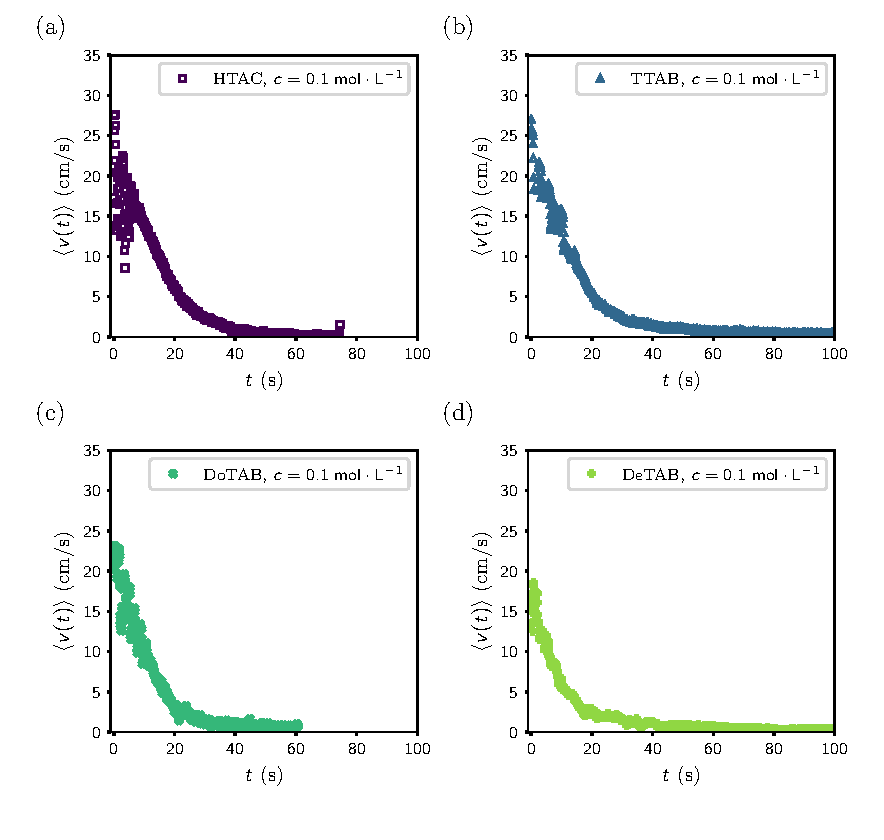
\includegraphics{./figures/Deceleration_vitesse_faible_concentration.pdf}
  %   \caption{Évolution de la vitesse moyenne $\langle v(t) \rangle$ au cours du temps pour quatre tensioactifs différents à la concentration initiale $c_0=0.1~\rm mol\cdot L^{-1}.$ (a) - HTAC CMC$= 1.3~\rm mM$. (b) - TTAB $\rm CMC = 4--5~\rm mM$. (c) - DoTAB $\rm CMC = 15~\rm mM$ (d) - DeTAB $\rm CMC = 65~\rm mM$.}
  %   \label{fig:DecelerationBateauMarangoni1}
  % \end{figure}

  % 



% \begin{figure}[!ht]
%   \centering
%   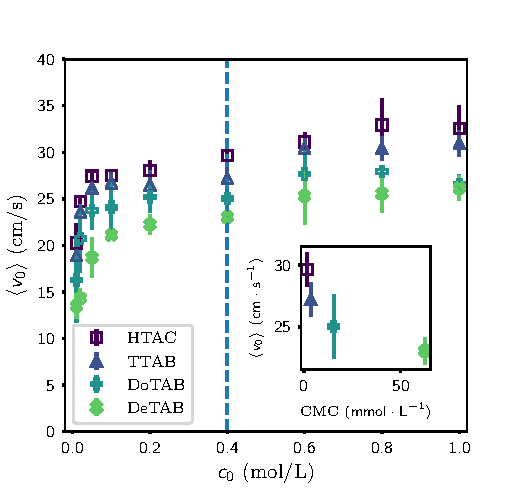
\includegraphics{./figures/Velocity_initial_051121.pdf}
%   \caption{Mesure de la vitesse $\langle v_0 \rangle $ en fonction de la concentration initiale pour les quatre tensioactifs. La sous-figure correspond à l'évolution de la vitesse en fonction de la CMC pour la concentration $c_0=0.4~\rm mol\cdot L^{-1}$ le long des pointillés.}
%   \label{fig:VitesseInitiale}
% \end{figure}
% % 
% % 

\subsubsection{Modélisation}

% \begin{wrapfigure}{r}{.5\textwidth}
% 	\centering
% 	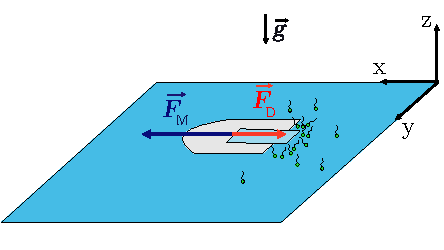
\includegraphics[width=.5\textwidth]{./figures/SchemaModeleBateau.pdf}
% 	\caption{Schéma de la modélisation du bateau de Marangoni}
% 	\label{fig:ModelSketchBateauMarangoni}
% \end{wrapfigure}

J'ai cherché à décrire l'évolution de la vitesse en fonction des paramètres qui sont: la concentration et la CMC du tensioactif. D'après nos résultats expérimentaux, les bateaux de Marangoni se déplacent spontanément sur la surface de l'eau. Dès que le bateau touche la surface, les tensioactifs s'étalent à l'arrière du bateau. Par conséquent, autour du bateau les tensioactifs sont plus concentrés à l'arrière qu'à l'avant, ce qui génère une différence de tension de surface le propulsant en avant. La force de propulsion qui s'applique au bateau est la différence de force capillaire entre l'avant et l'arrière du bateau dû à l'étalement des tensioactifs. Cette force est contrebalancée par les frottements entre l'eau et la coque du bateau. On applique la deuxième loi de Newton au système d'étude, c'est à dire un bateau se déplaçant dans le plan de la surface de l'eau (voir figure \ref{fig:schema}). La difficulté du problème réside dans la relation entre le gradient de tension de surface et le profil de concentration ainsi que la CMC liée à la nature du tensioactif. Pour résumer, en supposant que le système est à l'équilibre à chaque instant on peut relier la variation de la tension de surface à la concentration via les équations d'états de Langmuir et de Gibbs. On obtient ainsi $\Delta\gamma(r) = f(c, CMC)$, ce qui nous permet de connaître $F_{\rm propulsion} = \alpha L\Delta\gamma$. $\alpha$ est le facteur de forme du bateau, $L$ la longueur du bateau et $\Delta\gamma$ la différence de tension de surface entre l'avant et l'arrière du bateau. Pour la force de frottement, j'ai considéré la forme de la force de frottement établie pour une plaque rigide dans un écoulement intermédiaire entre le régime laminaire et turbulant ($Re\approx \num{1e3}$): $F_{D} = \beta v^{3/2}$ où $\beta$ est un coefficient qui dépend de la géométrie du bateau, de la viscosité de l'eau et de sa masse volumique. En appliquant la deuxième loi de Newton on obtient l'équation différentielle suivante à résoudre : 

\begin{equation}
  m\frac{\mathrm{d}v(t)}{\mathrm{d}t} + \underbrace{\beta v(t)^{3/2}}_{\rm frottements~visqueux} = \underbrace{\alpha L\Delta\gamma_0{\rm e}^{-\frac{t}{\tau_{\rm M}}}}_{\rm propulsion}.
  \label{eqn:differentielle}
\end{equation}

\begin{wrapfigure}[19]{r}{0.4\textwidth}
  \centering
  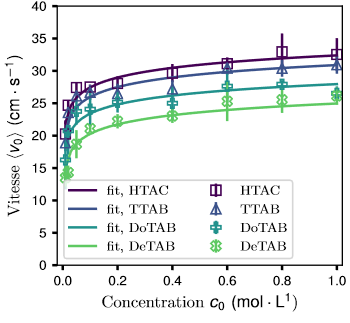
\includegraphics[width=.4\textwidth]{V0C.png}
  \caption{Comparaison entre modèle et expériences concernant la vitesse initiale en fonction de la concentration.}
  \label{fig:vitessevo}  
\end{wrapfigure}

Le terme en $\rm exp(-t/\tau_m)$ provient des observations expérimentales où la vitesse du bateau décroît de façon exponentielle. $\tau_{\rm M}$ est un temps caractéristique de décroissance de la vitesse du bateau. La résolution de l'équation différentielle nous donne une relation entre la vitesse initiale et les paramètres physicochimiques du système:

\begin{equation}
  v_0(c_0)=\left(\frac{\alpha RT\Gamma_{\rm max}}{0.664\rho l}\sqrt{\frac{L}{\nu}}\ln(1+K_{\rm L}c_0)\right)^{2/3}.
  \label{eqn:v0}
\end{equation}

Cette relation ajuste bien les données expérimentales. Et permet de mesurer les paramètres $\Gamma_\infty$ l'excès surfacique et $K_L$ la constante de Langmuir qui viennent des équations d'états de Langmuir et de Gibbs et collent avec la littérature [Rosen 2004]. Mon travail présente ici un premier modèle simple qui capture correctement les données expérimentales malgré les hypothèses utilisées pour le modéliser. J'ai eu l'occasion de présenter ce sujet d'étude à des étudiants de première au lycée Lycée Léonard de Vinci à Saint-Michel sur Orge. J'ai organisé des travaux pratique au cours desquels les étudiants ont construit leur dispositif, mesuré la vitesse en fonction de différents savons et étudier l'influence de la contamination de l'eau sur le mouvement du bateau. L'idée étant d'étudier l'influence de la pollution sur les déplacementsd'insectes à la surface de l'eau.

\subsection{Recherche pendant mon post-doctorat.}

J'ai été recruté en tant que post-doctorant par l'équipe Turbots du PMMH qui débutait un nouveau projet de recherche sur l'étude de la zone marginale glaciaire (Marginal Ice Zone en anglais ou MIZ), le but étant d'en réaliser un modèle expérimental à l'échelle du laboratoire. La MIZ est la zone où la banquise se réchauffe principalement, fond et se fragilise le plus. Dans cette région de la banquise, la houle océanique casse la banquise en fragments plus petits, accélérant la fonte de cette banquise. Jusqu'à présent les phénomènes d'interaction entre les vagues et la banquise ont été uniquement paramétrisées dans les modèles numériques climatiques planétaires. J'ai été recruté pour monter des expériences de laboratoire en mesure d'isoler et de reproduire les mécanismes physiques mis en jeu dans l'interaction entre la houle et la banquise. Le but étant d'obtenir des valeurs expérimentales pour vérifier les paramètres ajustables des modèles numériques.\medskip

Je me suis rapidement intégrer à l'équipe et  j'ai commencé à développer des outils d'analyse et de traitement de données basés sur une méthode de reconstruction de l'élévation de la surface de l'eau (synthetic schlieren) afin de mesurer l'amplitude des vagues et identifier les différents modes de déformation de la banquise en fonction de la fréquence et de l'amplitude des vagues. Ces outils numériques sont encore en développement et testés par l'équipe Turbots afin de publier. On peut trouver ces outils sur le lien suivant: \url{https://github.com/Turbotice/K-extraction}. Nous avons testé ces outils sur des modèles expérimentaux de \og{}banquise\fg{}. Pour comprendre les mécanismes de rupture de la banquise on a cherché des matériaux cassants. Un candidat qui semble reproduire le comportement de la banquise est un verni-colle en spray qui solidifie une fois posé sur l'eau. Il forme alors une croute qui se déforme sous l'effet de la houle jusqu'à une amplitude seuil où la croûte se brise. C'est une étude qui aujourd'hui fait l'objet d'une thèse, et depuis des expériences ont été menées à Rimouski dans la baie du Saint Laurent pour obtenir des données de terrain.

%La banquise est un matériau viscoélastique qui est capable de se déformer sur plusieurs mètres sans se casser, mais sous une certaine contrainte il peut se briser en deux. On a cherché des matériaux qui soient capables de se déformer mais aussi de se briser sous l'influence de la houle. Pour imiter le comportement élastique de la banquise on a commencé par utiliser des membranes commerciales dont on connaît l'épaisseur. De cette façon on peut connaître précisément les ondes qui se propagent dans ce type de membrane, en effet les relations de dispersion des ondes dans ces matériaux sont bien connues (thèse de Lucie Domino). 

\subsection{Travaux pratiques proposés à une classe de seconde sur la pollution des eaux}

Au cours de ma thèse j'ai eu l'occasion de présenter mes travaux de recherche dans différents lycées. À l'une de ces occasions, j'ai créé une activité sous forme de travaux pratiques à destinations d'une classe de seconde du lycée Léonard de Vinci à Saint-Michel sur Orge qui portait sur la pollution des eaux. Vous trouverez le document fourni aux élèves à travers ce lien cozy drive \url{https://gledoudic-drive.mytoutatice.cloud/public?sharecode=XdzAEUL3Ekut}.\medskip

Grâce à cette activité/TP, les élèves ont pu entrevoir comment un chercheur aborde une question. Les élèves ont dû formuler des hypothèses sur l'influence de la pollution des eaux sur le déplacement des microvelia à la surface d'une couche d'eau. Puis ils ont cherché une façon simple de tester leurs hypothèses en modélisant un insecte qui relargue des tensioactifs par le bateau en papier muni d'un petit réservoir à tensioactif. Ils ont observé le déplacement du bateau dans une eau propre et ont comparé la trajectoire observée à la trajectoire dans des eaux plus polluées (avec du poivre moulu, du savon dans l'eau, etc), jusqu'à émettre leurs propres conclusions.

\begin{figure}[ht]
  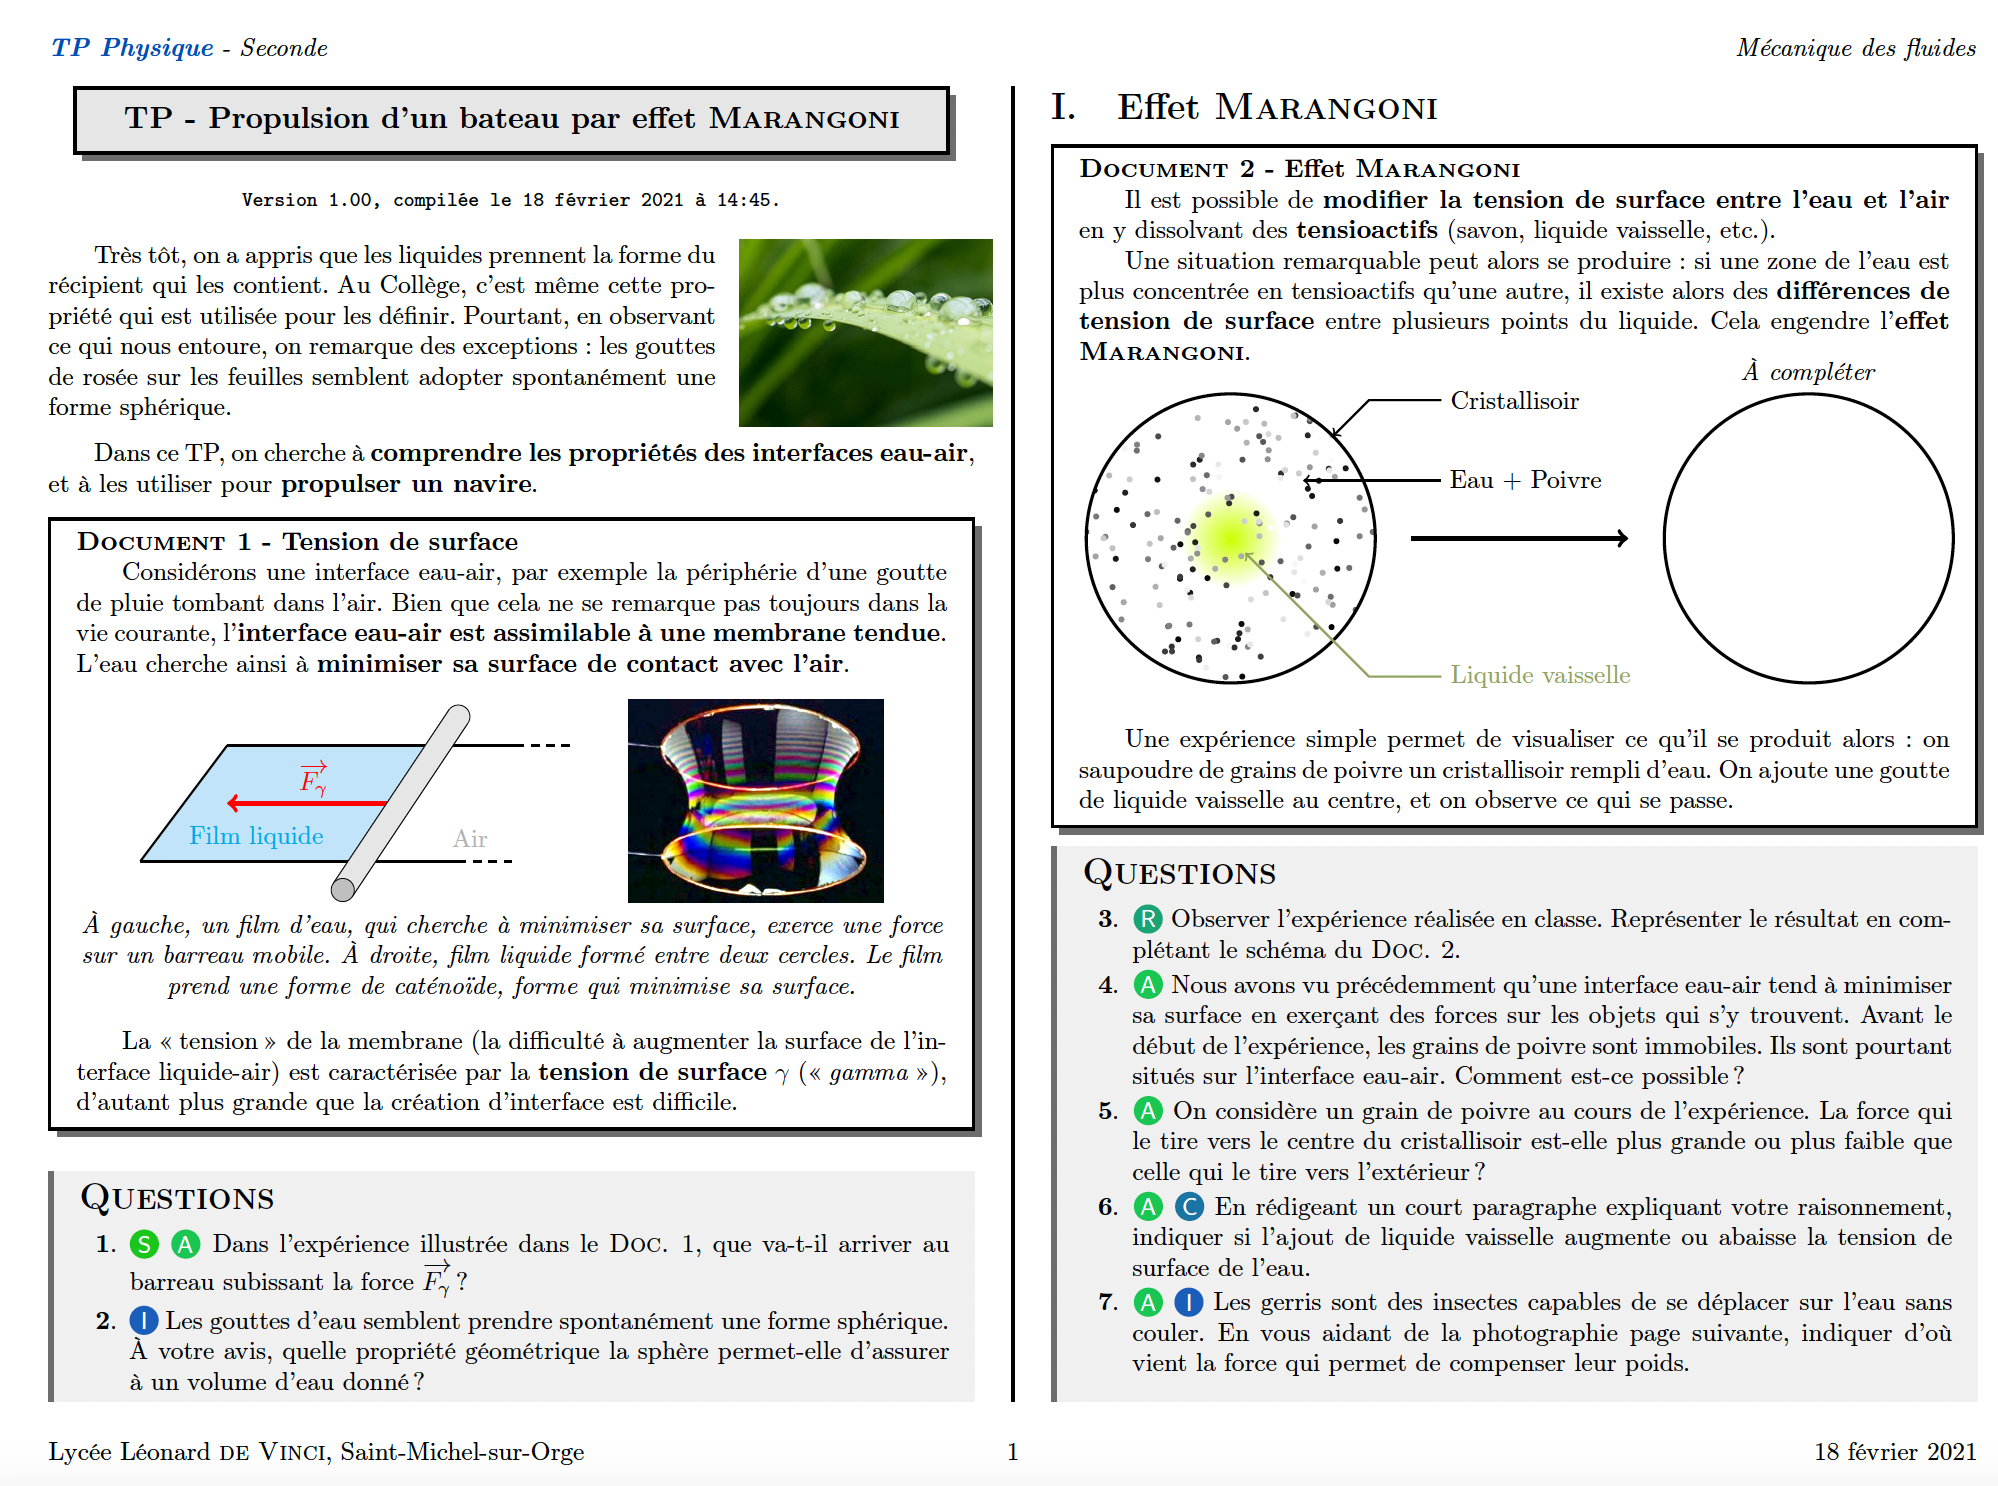
\includegraphics[width=.5\linewidth]{TP_Marangoni1.png}
  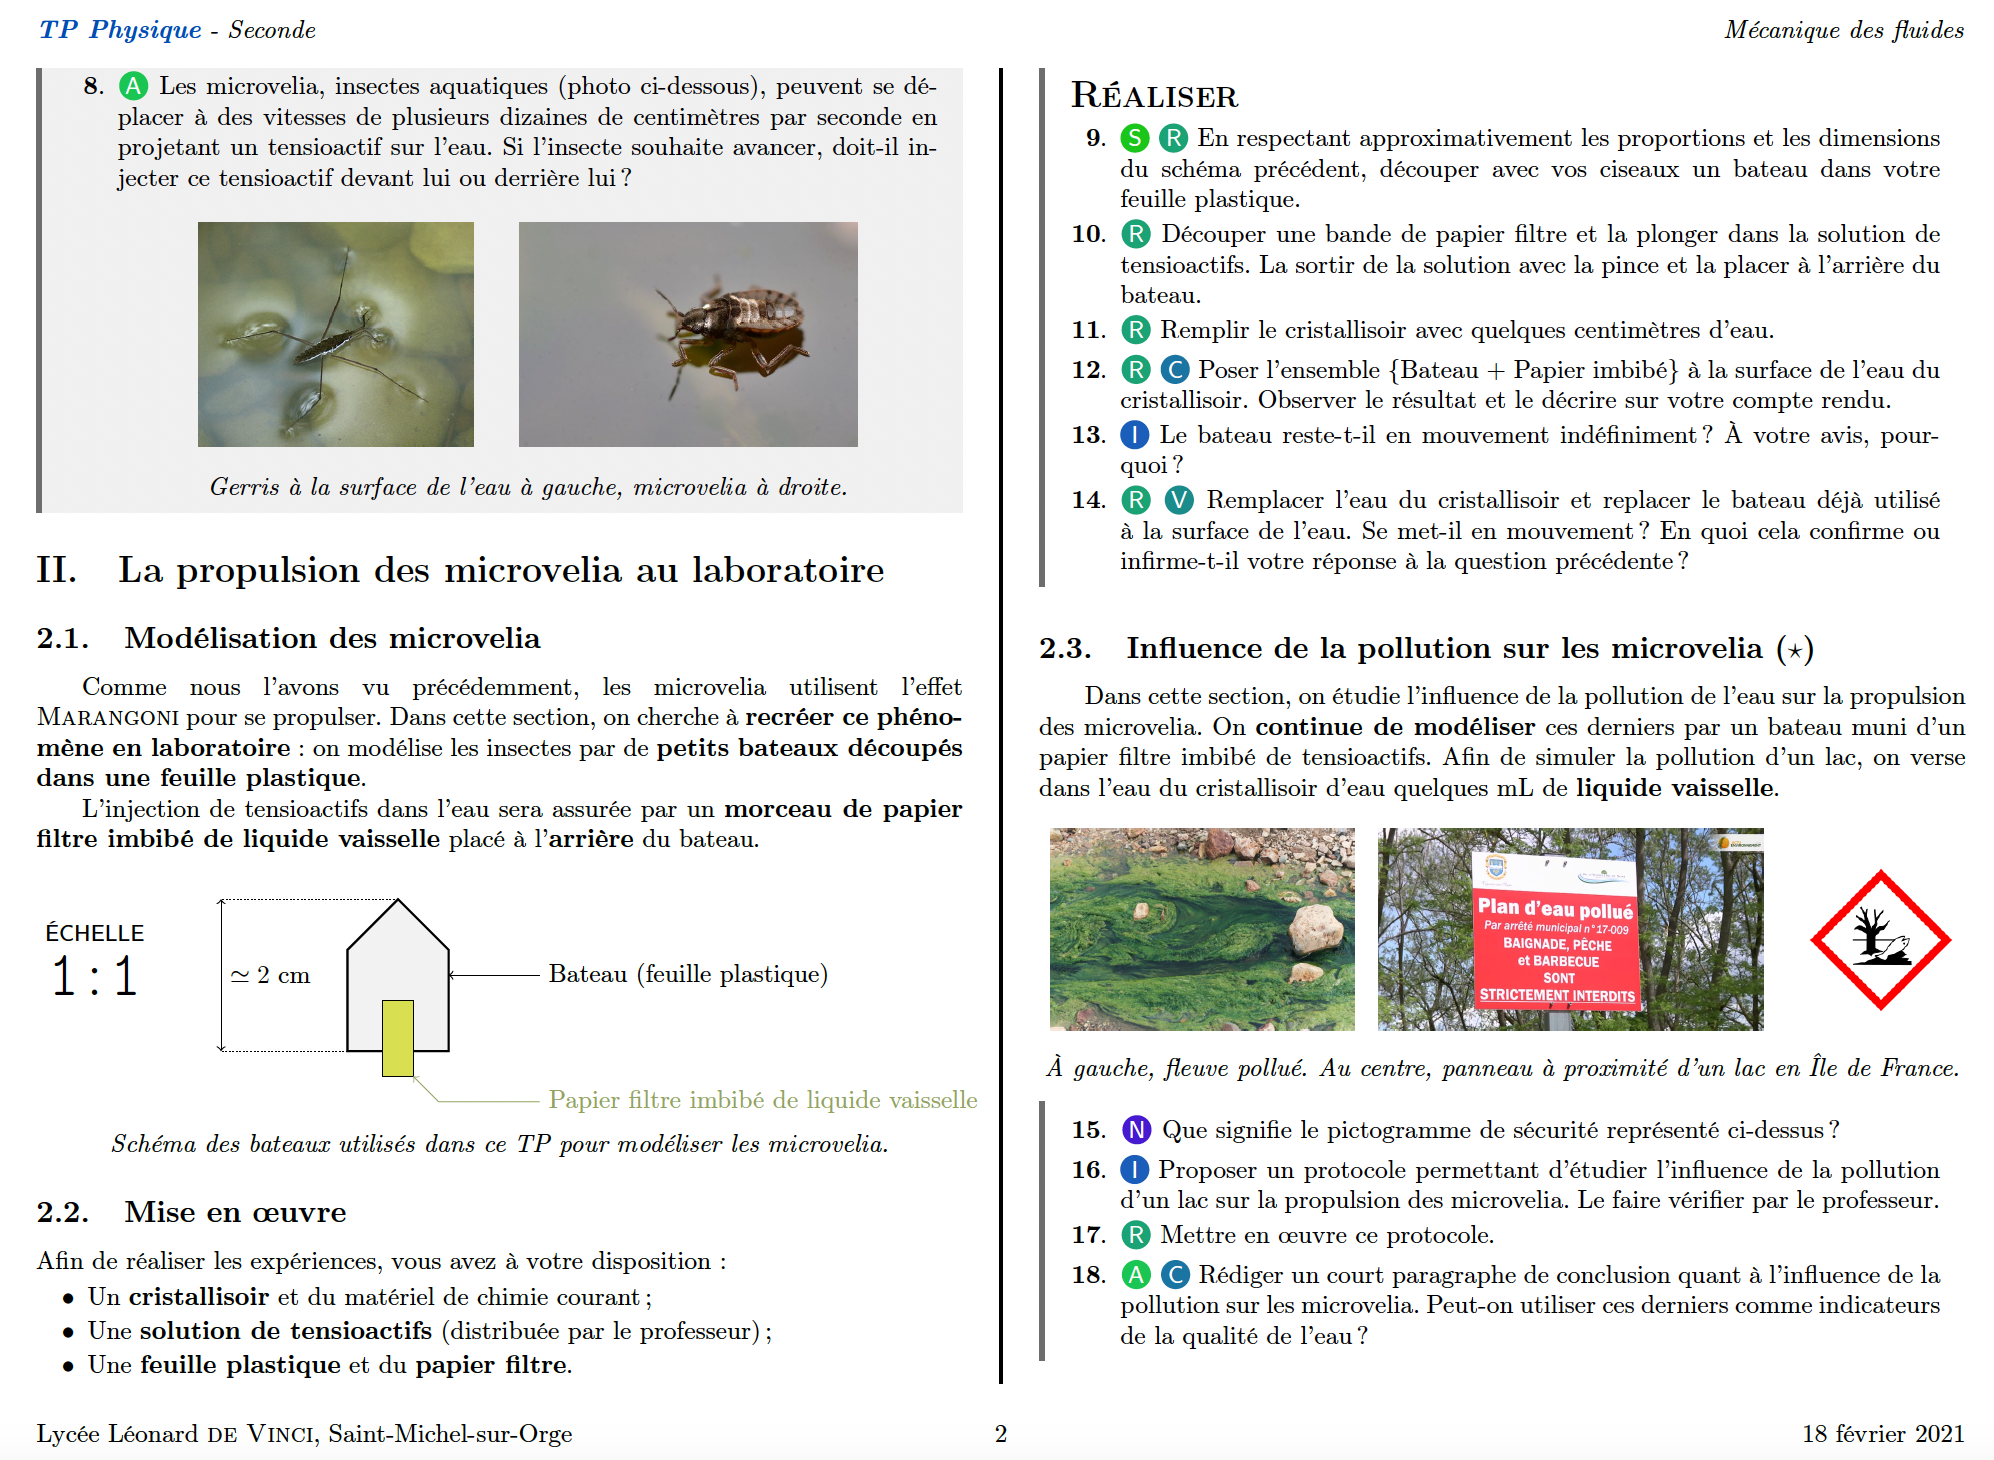
\includegraphics[width=.5\linewidth]{TP_Marangoni2.png}
  \caption{TP proposé aux secondes : \url{https://gledoudic-drive.mytoutatice.cloud/public?sharecode=XdzAEUL3Ekut}}
\end{figure}

\section{Vulgarisation scientifique}

En rapport avec le sujet de ma thèse, j'ai participé à la réalisation d'un projet de vulgarisation sur le thème de la tension de surface et de l'effet Marangoni. J'ai collaboré avec l'équipe de recherche en vulgarisation \og La Physique Autrement \fg{} basée au Laboratoire de Physique des Solides (LPS) à Orsay. Avec Marianne Cardon et Julien Bobroff et Matthieu Roché, nous avons lancé l'idée de créer un format vidéo qui a pour but de présenter la recherche en laboratoire autour de l'écoulement de Marangoni. J'ai mis en place des expériences illustrant l'influence de la tension de surface et de la force capillaire qui en découle. Vous pouvez trouver la vidéo en ligne à travers ce lien \url{https://dgxy.link/marangoni1}. Ce projet s'est conclu par le design d'un ensemble d'expériences simples permettant d'illustrer des phénomènes de tension de surface pour des présentations en grand public que l'on peut trouver sur un autre onglet du même site \url{https://dgxy.link/marangoni2}.\medskip


J'ai également organisé un atelier pour la fête de la science portant sur la propagation d'ondes à la surface de gouttes toriques mises en lévitation par effet Leidenfrost. Cet atelier est parti de travaux que j'ai mené pendant mon stage de Master 1 sur ce thème. C'est un travail que j'ai poursuivi en parallèle de ma thèse pendant ces trois dernières années et qui a donné lieu à deux publications. Pendant ma thèse, j'ai eu l'opportunité de venir présenter les travaux que j'ai mené au laboratoire dans deux lycées, notamment au lycée Lapérouse Kerichen à Brest devant des lycéens et des élèves de Classes Préparatoires, ainsi qu'au lycée Léonard de Vinci à Saint-Michel sur Orge. Pour l'occasion de ce dernier séminaire avec le professeur des étudiants M. Robin Hénaff, nous avons préparé des travaux pratiques sur la propulsion des bateaux de Marangoni (Mesure de vitesse de propulsion, influence de la pollution sur la propulsion des Microvelias).


\section{Enseignements}


\subsection{Mission doctorales d'enseignement à l'université de Paris Diderot}

Pendant ma thèse j'ai souhaité enseigner dans le cadre des missions doctorales. J'ai enseigné en première année de médecine (32 heures par an). Au cours de ces 96 heures j'ai parcouru le programme complet de physique de médecine, on a abordé les notions d'énergie potentielle, conservation de l'énergie mécanique, hydrostatique, écoulements parfaits ainsi que les pertes de charges dans une conduite (écoulement de Poiseuille), acoustique et imagerie, potentiel et champ électrostatique. Et pour compléter mon service j'ai également encadré des cours/TD de Physique en licence 1 de Sciences de la Vie et de la Terre (32 heures). Avec un programme similaire aux premières années de médecine avec un peu plus de mécanique du point.

\subsection{Fonctionnaire stagiaire à l'Éducation Nationale 2023-2024}

Cette année scolaire 2023-2024, est ma première année en tant que professeur de physique chimie (stagiaire) au lycée GT Jean Guéhenno à Fougères. J'enseigne à une classe de seconde et à trois classes de premières en enseignement scientifique.  C'est une année pendant laquelle j'ai pris beaucoup de plaisir à concevoir mes enseignements et à faire classe devant les élèves. J'ai aussi découvert la recherche en didactique et en pédagogie, j'ai essayé de m'y intéressé en expérimentant en classe de nouvelles façon d'enseigner comme la classe inversée qui consiste à laisser plus de place en classe à la résolution de problème plutôt qu'à l'apprentissage de notions de cours. \medskip

Je continue aussi à partager ma passion pour la recherche en montrant ce métier à mes élèves. J'ai eu l'opportunité d'inviter des chercheuses lauréates du concours L'Oréal Unesco : women in science à rencontrer mes élèves de seconde. Dr Alice Briole, Dr Suzanne Faure-Dupuy et Dr Lina El Hajji ont présenté leurs travaux en cours dans leurs laboratoires respectifs ainsi que le fonctionnement du monde de la recherche académique. Les élèves du lycée en ont également profité pendant un temps dédié à l'orientation pendant le midi ("les midis de l'orientation").  Les élèves ont beaucoup apprécié cet évènement, ce qui est ressorti le plus : c'était chouette de rencontrer des chercheuses, car c'est un métier qui est inconnu pour la majeure partie des élèves. Vous pouvez d'ailleurs trouver deux podcasts qui ont été réalisés par mes élèves à la suite de cet évènement \url{https://dgxy.link/podcast11} et \url{https://dgxy.link/podcast21}. Cet évènement a aussi été partagé dans les journaux tels que Ouest-France (\url{https://dgxy.link/2UEr6}).\medskip



\medskip



% Tout d'abord, pour décrire le déplacement du bateau nous écrivons l'équation de Newton, puis les équations d'état permettant de relier la variation de la tension de surface à la concentration. Ces équations nous permettront de faire le lien entre la propulsion du bateau et les effets physico-chimiques et thermodynamiques.
% % 

%    Le schéma ci-contre illustre le système étudié (voir figure \ref{fig:ModelSketchBateauMarangoni}). La cuve sur lequel le bateau se déplace se trouve dans le référentiel du laboratoire lié à la Terre et supposé galiléen. Le principe fondamental de la dynamique s'écrit:
  
%   \begin{equation}
% 	m\frac{d\vv{v}}{dt} = \sum_i{\vv{F_{\rm i}}}
% 	\label{eqn:Newton}
%   \end{equation}

%   % 
% Les forces perpendiculaires à la surface appliquées au bateau sont: le poids du bateau $\vv{P}=m\vv{g}$ et la force d'Archimède $\vv{P_{\rm A}} = -\rho_{\rm eau} V \vv{g}$. Avec $m$ la masse du bateau chargé de solution de tensioactif, $\vv{g}$ l'accélération de la pesanteur, $\rho_{\rm eau}$ la masse volumique de l'eau, et $V$ le volume déplacé par le bateau. Le bateau ne se déplace que dans le plan de la surface de l'eau, donc suivant l'axe vertical porté par $\vv{e_{\rm z}}$ la somme des forces verticales est à l'équilibre: 

% \begin{equation}
%   \rho_{eau} V g = mg \label{eq:SommeDesForcesVerticales}.
% \end{equation}

% En supposant que le volume de liquide déplacé correspond au volume du bateau immergé $V=L\times W \times \zeta$, nous pouvons calculer de combien le bateau déforme la surface de l'eau. L'équation \eqref{eq:SommeDesForcesVerticales} devient:
% \begin{equation}
%   \zeta = \frac{m}{\rho_{\rm eau} L W}
% \end{equation}
% Le bateau déforme la surface et s'enfonce de $z=100~\rm \upmu m$ ce qui est de l'ordre de l'épaisseur de la feuille transparente qui a permis de fabriquer le flotteur. Dans le plan de la surface de l'eau, les forces qui s'appliquent sur le bateau sont la force de propulsion liée à l'effet Marangoni notée $\vv{F_{\rm M}}$ et la force de frottement $\vv{F_{\rm D}}$ opposée au mouvement du bateau.

% \subsubsection{La force de frottement}

% Pour un objet plat, nous pouvons déterminer la force de frottement à partir de la structure de l'écoulement qui a lieu près d'une surface plane. Dans le référentiel du bateau, il est immobile et c'est l'eau qui s'écoule autour de lui et sous lui. Le régime d'écoulement est un régime intermédiaire entre le régime laminaire et le régime turbulent ($Re\approx 10^3$). Dans ces conditions la force de frottement sur une plaque rigide s'écrit : 
% \begin{equation}
%   F_{D} = \beta v^{3/2}.\label{eq:FrottementdePeau}
% \end{equation}

% $\beta$ est un coefficient qui dépend de la géométrie du bateau, de la viscosité de l'eau et de sa masse volumique.


% Pour cette démonstration nous nous plaçons dans le référentiel du bateau. Le bateau est donc immobile, et nous considérons l'écoulement qui a lieu autour de lui, en particulier sous la surface. Nous supposons que l'écoulement autour du bateau de Marangoni, est laminaire et uniforme de vitesse $U$ arrivant parallèlement à la plaque qui est le flotteur du bateau. L'écoulement est laminaire mais à grand nombre de Reynolds, car d'après nos mesures expérimentales $R_e$ est compris entre $2582$ et $6951$. Les gradients de vitesse et de vorticité sont concentrés près de la paroi et s'atténuent dans le temps. La distribution de la vorticité le long de la paroi s'élargit par diffusion visqueuse sur une distance $\delta(x)\approx \sqrt{\nu x/U}$, avec $\nu$ la viscosité cinématique du fluide et $x$ la position par rapport à l'arête de la plaque. $\delta$ représente l'épaisseur de la \textbf{couche limite} sur laquelle a lieu la transition entre l'écoulement de fluide loin du flotteur et près de celui-ci. L'écoulement au voisinage de la plaque est contrôlé par la viscosité qui impose une vitesse nulle à la paroi, il vient alors:
% 
% \begin{equation}
  % \frac{\delta(x_0)}{x_0} \approx \sqrt{\frac{\nu}{Ux_0}}\approx \frac{1}{\sqrt{Re_{x_0}}} \ll 1\label{eq:couchelimitebateau}.
% \end{equation}
% 
% $Re_{x_0}$ est le nombre de Reynolds local obtenu en prenant la distance $x_0$ à l'arête du flotteur comme échelle de longueur locale. Pour simplifier, nous étudions l'écoulement qui a lieu dans le plan ($xOz$) perpendiculaire à la surface de l'eau. Le bateau est en $z=0$. Nous supposons que l'écoulement est parallèle à la surface de l'eau, suivant la direction $Ox$.
% 
% \begin{wrapfigure}{l}{.5\textwidth}%[!ht]
  % \centering
  % 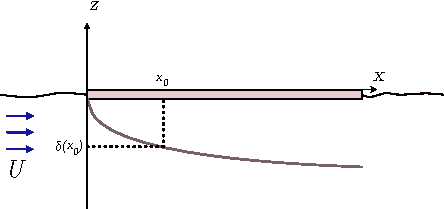
\includegraphics{./figures/couchelimitesketch.pdf}
  % \caption{Schéma de la couche limite le long du bateau de Marangoni. Inspiré de  \cite{Guyon2011}.}
  % \label{fig:SketchCouchelimite}
% \end{wrapfigure}
% 
% Dans la direction parallèle à la surface, la longueur caractéristique correspond à une distance $x_0$ à l'arête du flotteur. Perpendiculairement, la distance caractéristique correspond à l'épaisseur de la couche limite $\delta(x_0) \ll x_0$ défini dans l'équation \eqref{eq:couchelimitebateau}. Pour décrire le mouvement du fluide au voisinage du flotteur, nous écrivons l'équation de la conservation de la masse:
% 
% \begin{equation}
  % \frac{\partial v_x}{\partial x} + \frac{\partial v_z}{\partial z} = 0 \label{eq:consmass}.
% \end{equation}
% 
% \vspace{.5cm}\noindent Et les équations de Navier-Stokes dans les directions $x$ et $z$ s'écrivent:
% 
% \begin{equation}
  % \frac{\partial v_x}{\partial t} + v_x\frac{\partial v_x}{\partial x}+v_z\frac{\partial v_x}{\partial z} = -\frac{1}{\rho}\frac{\partial p}{\partial x} + \nu\left(\frac{\partial^2v_x}{\partial x^2}+\frac{\partial^2v_x}{\partial z^2} \right)\label{eq:NSx},
% \end{equation}
% et:
% \begin{equation}
  % \frac{\partial v_z}{\partial t} + v_x\frac{\partial v_z}{\partial x}+v_z\frac{\partial v_z}{\partial y} = -\frac{1}{\rho}\frac{\partial p}{\partial z} + \nu\left(\frac{\partial^2v_z}{\partial x^2}+\frac{\partial^2v_z}{\partial y^2} \right) \label{eq:NSz}.
% \end{equation}
% 
% $v_x$ et $v_z$ sont les composantes de la vitesse du fluide dans les directions $x$ et $z$ au voisinage de la paroi. $p$ est la pression dans le fluide et $\rho$ la masse volumique. À partir des équations \eqref{eq:consmass} et \eqref{eq:couchelimitebateau} nous pouvons simplifier les équations de Navier Stokes.
% 
% \begin{equation}
  % v_z\approx v_x\frac{\delta(x_0)}{x_0}\approx v_x. 
% \end{equation}
% 
% Nous en déduisons que:
% 
% \begin{equation}
% \frac{\partial^2v_x}{\partial z^2}\approx \frac{v_x}{\delta^2(x_0)} \gg \frac{v_x}{x_0^2} \approx \frac{\partial^2v_x}{\partial x^2},\label{eq:simplx}
% \end{equation}
% 
% ainsi que :
% 
% \begin{equation}
  % \frac{\partial^2v_z}{\partial z^2}\approx \frac{v_z}{\delta^2(x_0)} \gg \frac{v_z}{x_0^2} \approx \frac{\partial^2v_z}{\partial x^2}.\label{eq:simplz}
  % \end{equation}
  % 
% Par conséquent, nous pouvons réécrire les équations de Navier-Stokes stationnaire ($\partial/\partial t = 0$ \eqref{eq:NSx} et \eqref{eq:NSz} sous la forme simplifiée: 
% 
% \begin{equation}
  % v_x\frac{\partial v_x}{\partial x}+v_z\frac{\partial v_x}{\partial z} = -\frac{1}{\rho}\frac{\partial p}{\partial x} + \nu\frac{\partial^2v_x}{\partial z^2}\label{eq:NSx2},
% \end{equation}
% et:
% \begin{equation}
%  v_x\frac{\partial v_z}{\partial x}+v_z\frac{\partial v_z}{\partial y} = -\frac{1}{\rho}\frac{\partial p}{\partial z} + \nu\frac{\partial^2v_z}{\partial y^2} \label{eq:NSz2}.
% \end{equation}
% 
% Les trois termes correspondants à la variation de la vitesse $v_z$ sont négligeables devant les termes de l'équation \eqref{eq:NSx2}. De même, les fluctuations de pression dans la direction verticale $z$ ont une influence négligeable sur le profil de vitesse par rapport aux variations de pression dans la direction $x$. Par conséquent nous considérons que: $\partial p/\partial z = 0$ et que $p=p(x)$. De plus, en dehors de la couche limite, où les effets de la viscosité sont négligeables, nous pouvons écrire l'équation de Bernoulli le long d'une ligne de courant:
% 
% \begin{equation}
  % \frac{d p}{dx} +\rho U(x)\frac{dU(x)}{dx}=0\label{eq:Bernoulli}
% \end{equation}
% 
% En remplaçant l'équation \eqref{eq:Bernoulli} dans l'équation \eqref{eq:NSx2}, on obtient l'équation suivante:
% 
% \begin{equation}
  % v_x\frac{\partial v_x}{\partial x}+v_z\frac{\partial v_x}{\partial z} = U(x)\frac{dU(x)}{dx} + \nu\frac{\partial^2v_x}{\partial z^2}\label{eq:resNS},
% \end{equation}
% Maintenant, nous cherchons à déterminer l'équation différentielle vérifiée par le champ de vitesse à l'intérieur de la couche limite. Pour faire cela, nous exprimons la composante de la vitesse $v_x$ qui dépend de $x$ et $z$ en fonction de la variable adimensionnée $\theta$ définie comme $\theta = z/\sqrt{\nu x /U}$  et du module de la vitesse $U$.
% 
% \begin{equation}
  % v_x(x,z) = Uf(\theta)~~~~~~\text{et}~~~~~~\theta=\frac{z}{\sqrt{\nu x /U}}.
% \end{equation}
% 
% En remplaçant dans les équations \eqref{eq:consmass} et \eqref{eq:resNS}, on obtient l'équation de Blasius \cite{Guyon2011}:
% 
% \begin{equation}
  % f''(\theta) = -\frac{1}{2}f'(\theta)\int_0^{\theta}{f(\xi )d\xi}.
% \end{equation}
% 
% $f(\theta)$ décrit le profil de vitesse $v_x$ au voisinage de la paroi du flotteur comme illustré sur la figure \ref{fig:profilVitesse}.\bigskip 
% 
% \begin{wrapfigure}[15]{r}{.45\textwidth}%[!ht]
  % \centering
  % 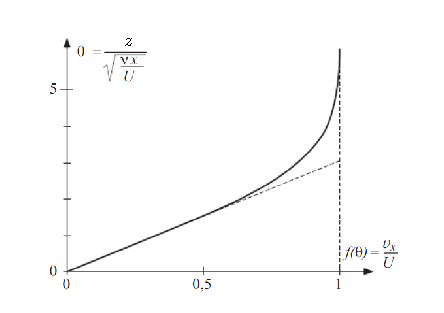
\includegraphics{./figures/profilecouchelimite.pdf}
  % \caption{Variation de la composante de vitesse en fonction de $\theta$.}
  % \label{fig:profilVitesse}
% \end{wrapfigure}
% 
% À partir de ces résultats nous pouvons déterminer la force de friction de peau entre le liquide et le flotteur du bateau de Marangoni. En effet, la force de frottement par unité de surface à une distance $x$ de l'arête est la composante $\tau_{xz}$ de la contrainte:
% 
% \begin{equation}
  % \begin{aligned}
    % \tau_{xz} &= \eta\left(\frac{\partial v_x}{\partial z}\right)_{z=0}=\eta U f'(0)\frac{\partial \theta}{\partial z}\\
    % \tau_{xz} &=\eta U f'(0)\sqrt{\frac{U}{\nu x}}.
  % \end{aligned}
% \end{equation}
% 
% Que nous pouvons réécrire en faisant apparaître, un terme en $U^2$ homogène à une pression:
% 
% \begin{equation}
  % \tau_{xz} = \rho U^2 f'(0)\sqrt{\frac{\nu}{U x}}.
% \end{equation}
% 
% Pour obtenir la force totale exercée par le fluide sur la plaque, nous intégrons $\tau_{xz}$ par rapport à $x$ et $y$ sur une des deux faces de la plaque plane de longueur L et de largeur $W$. Il vient alors :
% \begin{ombretheo}
  % \begin{theo}
    % \noindent \textbf{Force de friction sur la paroi du flotteur:}\bigskip
% 
    % \begin{equation}
      % F_{D} = \rho U^2f'(0)\sqrt{\frac{\nu}{U}}\displaystyle\int_{0}^{w}dy\int_{0}^{L}\frac{dx}{\sqrt{x}}=2\rho w U^2f'(0)\sqrt{\frac{\nu L}{U}} = \beta U^{3/2}.\label{eq:FrottementdePeau}
    % \end{equation}
% 
    %  Pour les calculs de la force, nous considérons que $L$ est la taille du flotteur dans la direction $Ox$ et que la vitesse $U$ est celle du flotteur, enfin $f'(0) \approx 1/3$ d'après Guyon \textit{et al} \cite{Guyon2011}.
% 
  % \end{theo}
% \end{ombretheo}
% 
% % 
% \subsubsection{La force de propulsion}
% % 
%  Déterminer l'expression de la force de Marangoni est une tâche ardue, car l'effet Marangoni dépend du gradient de concentration des tensioactifs lorsqu'ils s'étalent sur la surface de l'eau. Donc la force capillaire qui dépend de la variation de la tension de surface $\Delta\gamma$ dépend du temps et de l'évolution du profil de concentration $c(r,t)$. Nous proposons un modèle le plus simple possible en exprimant la force de propulsion comme une différence de force capillaire entre l'avant et l'arrière du bateau de la forme:
% 
%  \begin{equation}
%    F_{\rm M} = \alpha L\Delta\gamma(c(r,t),t). 
%  \end{equation}
% %  
%  $\alpha$ est un coefficient géométrique qui dépend de la forme du bateau. $\Delta\gamma$ est la différence de tension de surface entre l'avant et l'arrière du bateau. Nous faisons l'hypothèse que la concentration loin du bateau reste constante pendant toute la traversée du flotteur. De plus, la concentration surfacique de tensioactif au voisinage du bateau à $t=0$ lorsque le bateau touche la surface de l'eau est celle de la solution de tensioactifs dans le réservoir c'est à dire $c(r=0~\rm m,t=0~\rm s) = c_0$.\bigskip
% % 
%  Ces hypothèses sont fortes, car en pratique la surface de l'eau est rapidement contaminée lors du dépôt du tensioactif donc la concentration loin du bateau devient non-nulle $c_{\infty} \neq 0$. Nous décomposons la variation de la tension de surface en un produit d'une fonction qui dépend de la concentration initiale de tensioactif et d'une fonction qui dépend du temps:
% % 
% \begin{equation}
%   \Delta\gamma(t) = \chi(c_0)\times \xi(t) = \Delta\gamma_0(c_0)\times \xi(t)
% \end{equation}

% On cherche à exprimer la variation de la tension de surface en fonction des paramètres thermodynamique, qui suppose que le système est à l'équilibre thermodynamique à chaque instant. Les équations d'états de Langmuir et de Gibbs nous permettent de donner l'expression suivante pour $\Delta\gamma$:
% % 
% Nous avons vu avec la thermodynamique de l'adsorption des molécules tensioactives qu'il est possible d'obtenir des relations entre la variation de la tension de surface et la concentration en tensioactifs. Nous avions défini l'isotherme de Langmuir (eq. \eqref{eq:Langmuir}) que nous rapellons ici: 
% % 
% \begin{equation}
%   \Delta\gamma(c_0) = RT\Gamma_{\infty}\ln{1+K_{\rm L}c_0}
% \end{equation}

% avec :
% Cette équation d'état caractérise la variation de la tension de surface lorsqu'un tensioactif est ajouté à l'interface entre deux fluides. Nous choisissons cet isotherme car il prend en compte la saturation de l'interface via la concentration surfacique maximale $\Gamma_{\infty}$. La concentration surfacique maximale est reliée à la concentration en volume et la concentration surfacique à travers l'équation \eqref{eq:IsothermeLangmuir} que nous rappelons aussi ci-dessous:
% % 
% \begin{equation}
%   \Gamma(c) = \Gamma_{\infty}\frac{K_{\rm L}c}{1+K_{\rm L}c}.
% \end{equation}





% Ainsi la force motrice s'écrit :
% R est la constante des gaz parfaits $R = 8.314~\rm J\cdot K^{-1}\cdot mol^{-1}$, $T$ la température en Kelvin (K). $K_{\rm L}$ est la constante de l'équilibre d'adsorption de Langmuir, qui mesure l'efficacité du tensioactif à changer la tension de surface \cite{Chang1994}. Pour finir, nous supposons que $\xi(t)$ est de la forme d'une exponentielle décroissante, car les résultats expérimentaux suggèrent que la vitesse du bateau décroît exponentiellement avec le temps (voir figure \ref{fig:DecelerationBateauMarangoni1}), il vient:
% % 
% \begin{equation}
%   F_{\rm M} = \alpha \Delta\gamma_0(c_0){\rm e}^{-\frac{t}{\tau_{\rm M}}}= \alpha LRT\Gamma_{\rm max}\ln(1+K_{\rm L}c_0){\rm e}^{-\frac{t}{\tau_{\rm M}}}.
% \end{equation}


% \subsection{Résolution de l'équation}

% \subsubsection{Équation stationnaire}

% Dans un premier temps, nous résolvons l'équation stationnaire afin de déterminer la vitesse initiale du bateau $v_0$ lorsque les forces de frottement et de propulsion sont à l'équilibre. L'équation stationnaire est la suivante:

% \begin{equation}
%   \beta v_0^{3/2} = \alpha L\Delta\gamma(c_0).\label{eq:stationnaire}
% \end{equation}


% En isolant d'un côté de l'équation la vitesse $v_0$ il vient directement l'expression de la vitesse initiale en fonction de la concentration:

% \begin{equation}
%   v_0(c_0)=\left(\frac{\alpha RT\Gamma_{\rm max}}{0.664\rho l}\sqrt{\frac{L}{\nu}}\ln(1+K_{\rm L}c_0)\right)^{2/3}.
%   \label{eqn:v0}
% \end{equation}

% Les valeurs de la concentration surfacique maximale $\Gamma_{\infty}$ sont tabulées dans la littérature pour de très nombreux tensioactifs et sont reportées dans le tableau \ref{TABLE:Paramv0} les valeurs présentées dans la littérature \cite{Rosen, Kosaka2008}. En ce qui concerne $K_{\rm L}$ la constante d'équilibre d'adsorption des tensioactifs de l'isotherme de Langmuir est plus difficile à trouver dans la littérature. Néanmoins, nous avons trouvé la valeur de $K_{\rm L}$ pour trois tensioactifs de la famille des TAB reportés par Nguyen \textit{et al} \cite{Nguyen2017}: $\rm C_{14}TAB$, $\rm C_{15}TAB$, $\rm C_{16}TAB$ qui sont indiquées dans le tableau \ref{TABLE:Paramv0} déterminées pour un système à l'\textbf{équilibre}. Nous utiliserons $K_{\rm L}$ et $\alpha$ comme paramètres d'ajustement du modèle afin de le comparer aux expériences.

% % \begin{table}[ht!]
% %   \centering
% %   \begin{tabular}{c|c|c|c}
% %     \hline \hline
% %     Tensio-actifs & $\Gamma_{\infty}~\rm (mol\cdot m^{-2})$ & Tensioactifs  &$K_{\rm L }~\rm (m^{3}\cdot mol^{-1})$ \\ \hline \hline
% %     HTAC, $\rm C_{16}TAC$  & $3.4\cdot 10^{-6}$ &$\rm C_{16}TAB$ & $2.017$ \\ 
% %     TTAB, $\rm C_{14}TAB$  & $3.3\cdot 10^{-6}$ &$\rm C_{15}TAB$ &$1.5$ \\ 
% %     DoTAB, $\rm C_{12}TAB$  & $2.9\cdot 10^{-6}$ &$\rm TTAB, C_{14}TAB$ &$1.2$ \\ 
% %     DeTAB, $\rm C_{10}TAB$  & $2.8\cdot 10^{-6}$ & &\\  \hline
% %   \end{tabular}
% %   \caption{Valeurs tabulées dans la littérature pour la concentration surfacique maximale $\Gamma_{\infty}$, source: \cite{Rosen, Kosaka2008}. Ainsi que pour la constante d'adsorption de Langmuir $K_{\rm L}$, source:\cite{Nguyen2017}.}
% %   \label{TABLE:Paramv0}
% % \end{table}

% La comparaison entre les résultats expérimentaux et le modèle sont présentés sur la figure \ref{fig:modelev0}. En ajustant $\alpha=0.15$ ainsi que $K_{\rm L}$ pour chaque tensioactif, nous obtenons un bon accord entre les courbes et les résultats expérimentaux. L'ajustement de $K_{\rm L}$ nous permet d'obtenir les valeurs indiquées sur le tableau \ref{TABLE:resAjustement} pour les quatre tensioactifs utilisés. Malheureusement, nous ne pouvons pas comparer pour les quatre tensio-actifs à la littérature existante car nous n'avons trouver que des valeurs pour le $C_{14}TAB$.


% \begin{figure}[!ht]
%   \centering
%   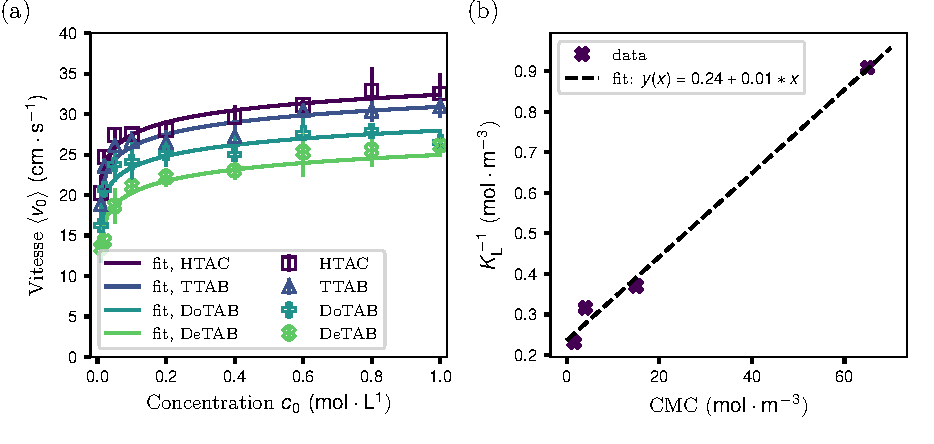
\includegraphics[scale=.8]{./figures/Vitesse_initiale_versus_concentration_modele.pdf}
%   \caption{Comparaison entre les mesures de la vitesse initiale avec le modèle}
%   \label{fig:modelev0}
% \end{figure}

% \begin{table}[ht!]
%   \centering
%   \begin{tabular}{ccc}
%   \hline \hline
%   Tensioactif & $K_{\rm L}$ $\rm(m^{3}\cdot mol^{-1})$ ajusté & $K_{\rm L}$ $\rm(m^{3}\cdot mol^{-1})$ littérature \\ \hline \hline
%   HTAC, $\rm C_{16}TAC$ & $4.4$ & NA \\
%   TTAB, $\rm C_{14}TAB$ & $3.2$ & $1.2$ \\
%   DoTAB, $\rm C_{12}TAB$ & $2.7$ & NA \\
%   DeTAB, $\rm C_{10}TAB$ & $1.1$ & NA \\ \hline \hline
%   \end{tabular}
%   \caption{Résultats des ajustements du coefficient d'adsorption de Langmuir $K_{\rm L}$.}
%   \label{TABLE:resAjustement}
% \end{table}

%   Nous remarquons qu'il y a un facteur $3$ entre la valeur que nous obtenons et la littérature. Malgré cet écart, l'évolution de $K_{\rm L}$ avec la CMC semble cohérente. En effet pour une concentration donnée, plus la vitesse est grande plus $K_{\rm L}$ est grand. De la même manière, plus la CMC est petite plus $K_{\rm L}$ est grand (voir figure \ref{fig:modelev0}\textcolor{blue}{(b)}). Ce graphique traduit l'évolution de l'efficacité des tensio-actifs en fonction de leur nature et de leur affinité avec l'interface. D'après Chang \textit{et. al} \cite{Chang1994}, plus la molécule étudiée présente une valeur élevée de $K_{\rm L}$ plus elle est efficace. C'est effectivement ce que nous observons, Le tensioactif HTAC qui est le plus efficace pour propulser les bateaux obtient la plus grande valeur de $K_{\rm L}$. Et inversement, le DeTAB est le tensioactif qui présente les vitesses les plus faibles et obtient la valeur de $K_{\rm L}$ la plus faible.\bigskip

% La réponse linéaire entre $1/K_{\rm L}$ et la CMC rappelle les tendances observées dans la littérature \cite{Gilanyi2008}. Cependant Rosen a montré que l'efficacité d'un tensio-actif est dominée par la tête hydrophile du tensioactif \cite{Rosen}, donc tous les $\rm C_{\rm n}TAB$ devraient présenter la même efficacité. Ces résultats sont vrais si la chaîne hydrocarbonée était orientée parfaitement perpendiculairement à l'interface. Cependant, des études plus récentes montrent que les arrangements des tensio-actifs adsorbés sont plus compliqués que cela. La tête hydrophile $\rm Br^{-1}$ peut interagir avec les hydrocarbones ce qui induit des réarrangements de la géométrie de la monocouche de tensioactif à l'interface. Les auteurs montrent que cela joue un rôle significatif sur l'adsorption des tensioactifs \cite{Lyttle1995, Belleffect1998}. À ces effets, s'ajoutent des phénomènes d'interaction entre ions et contre ions qui peuvent avoir une influence sur l'adsorption \cite{Wangsurfactant2013}. Les résultats montrent que l'efficacité du tensioactif est fortement corrélée à la longueur de la chaîne carbonée: elle augmente non-linéairement avec la longueur de la chaîne \cite{Nguyen2017}. C'est ce que nous observons sur la figure \ref{fig:modelev0}\textcolor{blue}{(b)} où nous avons tracé $K_{\rm L}$ en fonction de la CMC sachant que la longueur de la CMC augmente avec le nombre de chaînes carbonées.



% \subsubsection{Résolution de l'équation temporelle}

% % Dans cette section nous proposons de résoudre l'équation temporelle: 
% % 
% \begin{equation}
%   m\frac{\mathrm{d}v(t)}{\mathrm{d}t} + \beta v(t)^{3/2} = \alpha L\Delta\gamma_0{\rm e}^{-\dfrac{t}{\tau_{\rm M}}}.
% \end{equation}
% 
% Cette équation est difficile à résoudre à la main à cause de la force de frottement qui est proportionnelle à $v^{3/2}$.  Par conséquent, nous cherchons une solution numérique à l'aide de Python et la fonction odeint de la librairie Scipy \cite{2020SciPy-NMeth}. Pour résoudre cette équation, nous utilisons les paramètres tabulés dans la littérature pour $\Gamma_{\rm max}$ et calculés pour $K_{\rm L}$. Le paramètre géométrique $\alpha$ est conservé $\alpha= 0.15$. Pour comparer la solution numérique temporelle de la vitesse aux données expérimentales nous ajusteront le paramètre noté $\tau_{\rm M}$ qui correspond au temps caractéristique de décroissance de l'exponentielle. Nous comparons les résultats numériques aux données expérimentales sur la figure \ref{fig:decroissancemodele}. Il faut remarquer que le modèle capture assez bien les résultats expérimentaux aux faibles concentrations. Aux grandes concentrations, nous pouvons voir sur la figure \ref{fig:decroissancegrandeconcentrationmodele} que ce n'est pas tout à fait le cas, notamment pour le HTAC et le TTAB qui présentent des paliers pendant la décroissance de la vitesse. Nous n'avons pas d'explication exactes pour ces paliers à l'heure actuelle, nous supposons que c'est un effet de la saturation de l'interface lorsque le réservoir du bateau est très concentré, car ces paliers ne sont pas présents aux concentrations plus faibles. L'ajustement des solutions de l'équation semble mieux marcher pour le DoTAB et le DeTAB. Par conséquent, nous en déduisons la variation de la tension de surface en fonction d'une exponentielle du temps semble une bonne hypothèse pour décrire son évolution au cours du temps.\bigskip
% 
% 
% \begin{figure}[!ht]
  % \centering
  % 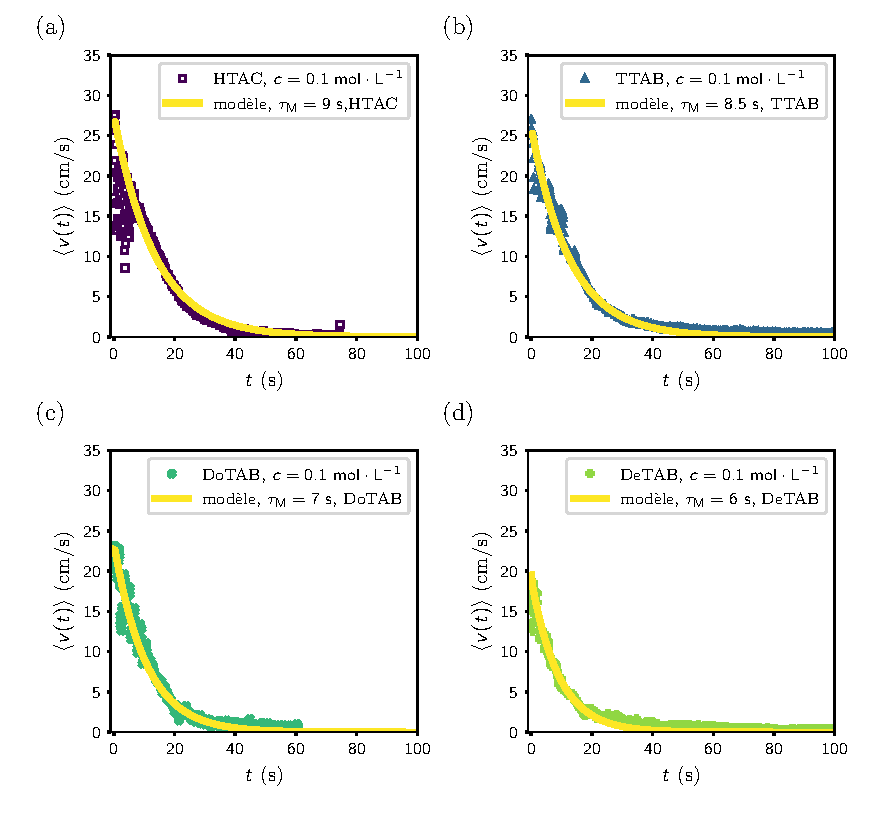
\includegraphics{./figures/Deceleration_vitesse_faible_concentration_modele.pdf}
% 
  % \caption{Comparaison entre les profils de vitesse expérimentaux et les solutions numériques de l'équation différentielle pour les quatre tensioactifs.}
  % \label{fig:decroissancemodele}
% \end{figure}
% 
% \underline{\textbf{Ce que nous retenons:}}\medskip
% 
    % Bien que le modèle que nous proposons soit très simplifié, nous parvenons à décrire les effets de la thermodynamique sur la propulsion du bateau de Marangoni.\bigskip
% 
    % Cependant il nous faut discuter de deux points que nous avons omis dans notre modèle. En effet, nous avons pu remarquer des émissions d'ondes lorsque le bateau se déplace à la surface de l'eau. Or, les ondes sont une source de dissipation d'énergie et donc doivent être prises en compte pour modéliser la propulsion des bateaux. Dans un second temps nous allons discuter de l'influence de l'écoulement de Marangoni sur la propulsion de nos bateaux, car nous avons vu que l'effet de l'écoulement était non-trivial.\medskip
% % 
% \begin{Programme}{Établir l'équation du mouvement d'un objet propulsé}
%   On peut proposer aux étudiants de classes préparatoires ou même de lycée d'établir l'équation de mouvement des bateaux de Marangoni. Avec comme applications la propulsion de petits insectes à la surface d'une surface d'eau comme un bassin.\medskip

% 	\begin{enumerate}
%     \item Description des forces appliquées au système (verticales et horizontales);
%     \item On peut discuter du poids du Bateaux versus la poussée d'archimède (au programme du lycée);
% 		\item On donne la forme de la force de propulsion, amplitude et direction, on peut la simplifier en prenant une force de propulsion constante avec un certain réservoir (analogie à la fusée);
% 		\item illustration de la 3ème loi de Newton.
% 		\item Discuter de la force de frottement, au lycée on peut donner la forme proportionnelle à la vitesse. En CPGE on peut arriver à discuter de la dépendance de la force de frottement en fonction du régime de vitesse, nombre de Reynolds; 
%     \item CPGE : vidange du réservoir de tensioactifs (analogie avec le réservoir de carburant d'une fusée)
% 		\item échelle caractéristique de diffusion.
% 		\item On peut choisir ainsi différents niveaux de description du problème en restant dans le programme adapté au niveau des étudiants et résoudre l'équation du mouvement avec différents degrés de difficulté et même proposer une modélisation du problème à l'aide de programmes pythons que l'on pourra discuter à la lumière de résultats expérimentaux obtenus en travaux pratiques.
% 	\end{enumerate}

%   Enfin, avec l'exemple de la propulsion des microvellia à la surface de l'eau grâce au relargage de tensioactif est l'occasion de réaliser un travail expérimental où l'étudiant peut fabriquer un support en papier ou en plastique avec un moteur (languette de papier filtre imbibée de tensioactif) et mesurer la vitesse de propulsion du bateau à l'aide d'une caméra et d'avimeca ou de regressi en pointant la position du mobile. On peut également sensibilsier les étudiants aux effets de la pollution qui restent à la surface des étants. En effet une surface d'eau polluée a une tension de surface plus faible que l'eau propre et donc l'effet des tensioactifs est plus faible voir nul. Les insectes ne peuvent alors plus se nourrir, fuir de leurs prédateurs, etc. 

% \end{Programme}
% % 
% Enfin, il est important de remarquer que dans nos expériences les variations du champ de concentration à la surface sont dominées par le transport induit par l'écoulement de Marangoni et non pas par la diffusion des molécules dans l'eau. En effet le nombre de Péclet s'écrit: 
% % 
% \begin{equation}
%   P_e = \frac{L_{\rm bateau}v_{\rm bateau}} {D} \label{eq:NombreDePeclet}
% \end{equation}
% % 
% En prenant comme longueur caractéristique la longueur du bateau $L=2~\rm cm$, pour la vitesse nous prendrons la vitesse initiale du bateau $v_0$ et $D$ le coefficient de diffusion des molécules dans l'eau $D=1\cdot 10^{-10}~\rm m^2\cdot s^{-1}$, nous obtenons un nombre de Péclet compris entre $P_e\in\left[5\cdot 10^4, 4\cdot 10^{6}\right]$ ce qui est extrêmement grand. Outre cela, nous pouvons comparer nos données expérimentales aux simulations de Ender \textit{et al}.Pour cela nous allons calculer le Nusselt en suivant leur définition \eqref{Nusselt}. Cette équation est obtenue numériquement en supposant que le flux de tensioactifs sortant du réservoir est constant. Le nombre de Nusselt caractérise le taux de flux émis par rapport au flux diffusif de tensioactifs.
% % 
% \begin{equation}
%   \rm Nu = \left\{
%   \begin{array}{ll}
%     1+\frac{1}{2}\bar{v}+... &~\mbox{pour}~\bar{v}\ll 1\\
%     0.6245\bar{v}^{1/3}       &~\mbox{pour}~\bar{v}\gg 1
%   \end{array}
%   \right.\label{Nusselt}
% \end{equation}
% 
% $\bar{v}$ est déjà un nombre de Péclet car ils le définissent comme $\bar{v} = L v/D$. Lorsque $\mathrm{Nu}= 1$ le bateau ne se déplace pas et l'étalement des tensioactifs est purement diffusif. Dès que le bateau est propulsé $\mathrm{Nu}>1$, le transport des molécules domine sur la diffusion. Nous avons tracé sur la figure \ref{fig:NusseltPeclet}\textcolor{blue}{(a)} les résultats numériques de Ender \textit{et al} et le calcul du Nusselt pour nos paramètres expérimentaux. Nous voyons que toutes nos données expérimentales se retrouvent dans la région dominée par le transport des molécules et non pas dans le régime diffusif.
% % 
% \begin{figure}[!ht]%[10]{r}{.5\textwidth}
%   \centering
%   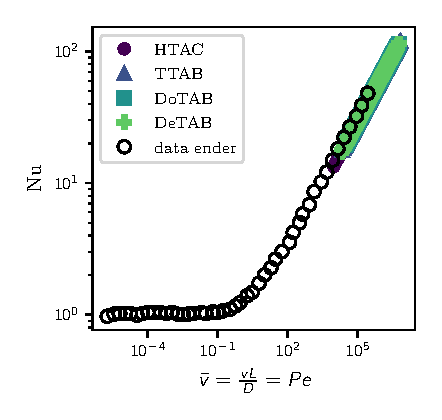
\includegraphics[scale=1]{./figures/Nusselt.pdf}
%   \caption{Comparaison des calculs du nombre de Nusselt aux résultat analytiques et numériques de Ender \textit{et. al} \cite{Ender2021}}
%   \label{fig:NusseltPeclet}
% \end{figure}
% 
% \subsubsection{Conclusion}
% 
% Ondes source de frottement, mesure de l'écoulement autour du bateau, régime de transport des tensioactifs. Ajouter les documents apportés en lycée. 
% \section{Propagation d'ondes à la surface de gouttes en lévitation}
% 
% Nous avons étudié la propagation d'ondes à la surface de gouttes d'eau cylindriques maintenue en lévitation sur leur propre vapeur par l'effet Leidenfrost (ou caléfaction) et sur des substrats superhydrophobes \cite{pham2020surface, le2021surface}. En règle générale, la taille des gouttes en lévitation est limitée. En effet, lorsque les gouttes dépassent une certaine taille le film de vapeur ne parvient plus à s'échapper uniquement par les bords de la goutte, mais vient percer la goutte et la rendre instable.\bigskip
% 
% Cependant il est possible de dépasser la limite en taille en choisissant un bon support. Par exemple en déposant des gouttes sur un substrat courbé il est possible d'obtenir des gouttes en forme de tore par caléfaction \cite{perrard2012leidenfrost}. Cela a permis de mettre en lumière des effets spectaculaires comme l'apparition de motifs géométriques. ces motifs résultent de l'apparition d'ondes de surface de forme polygonale qui brisent la symétrie du tore.\bigskip
% 
% Dans ce contexte, nous avons débuté des expériences similaires dans une géométrie linéaire. Les gouttes sont déposées sur un substrat en forme de gouttière rectiligne (de $45$ cm de long) et chauffé à $250^{\circ}~\rm C$. Les gouttes sont tirées et piégées à chaque extrémité du canal pour qu'elles ne puissent pas se rétracter sous l'effet de la tension de surface. Nous avons perturbé le système en générant des ondes sur la goutte à l'aide d'un batteur et d'un pot vibrant \ref{fig:batteur}.
% 
% \begin{figure}[!ht]
%   \centering
%   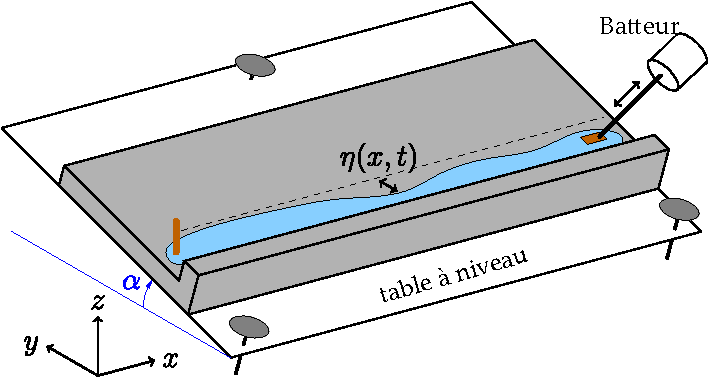
\includegraphics{./figures/Leidenfrost/schemaleidenfrost.pdf}
%   \caption{Schéma du dispositif expérimental}
%   \label{fig:batteur}
% \end{figure}
% \begin{wrapfigure}{r}{.5\textwidth}
  % \centering
  % 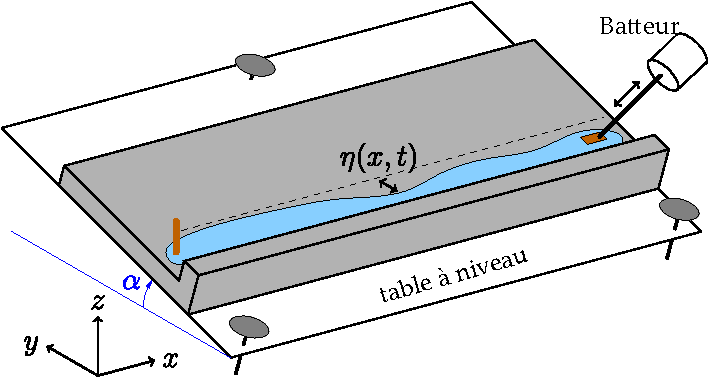
\includegraphics[width=.5\textwidth]{./figures/Leidenfrost/schemaleidenfrost.pdf}
  % \caption{Schéma du dispositif expérimental}
  % \label{fig:batteur}
  % \end{wrapfigure}
% Nous avons réalisé ces expériences en caléfaction mais aussi sur un substrat superhydrophobe plus simple à mettre en place. Pour cela, deux substrats ont été usinés, un en forme de $L$, qui posé sur la table à niveau peut être incliné d'un angle $\alpha$ entre $0^{\circ}$ et $45^\circ$, et l'autre en forme de V symétrique avec un angle $\alpha=10^\circ$ avec l'horizontale (voir figures \ref{fig:Leidenphoto}\textcolor{blue}{a,b}). Les deux substrats sont traité par un revêtement super-hydrophobe Never-Wet qui permet d'obtenir des angles de contact de $160^\circ$. Lorsque le batteur est mis en marche, nous pouvons voir différents modes de propagation d'ondes à la surface de la goutte (voir figures \ref{fig:Leidenphoto}\textcolor{blue}{(c,d)}). Nous voyons sur ces figures des modes variqueux et sinueux. En mesurant la déformation de la surface de la goutte, nous avons caractériser les différents modes de propagation en traçant les relations de dispersion des ondes observées.
% 
% \begin{figure}[!ht]
    % \centering
    % 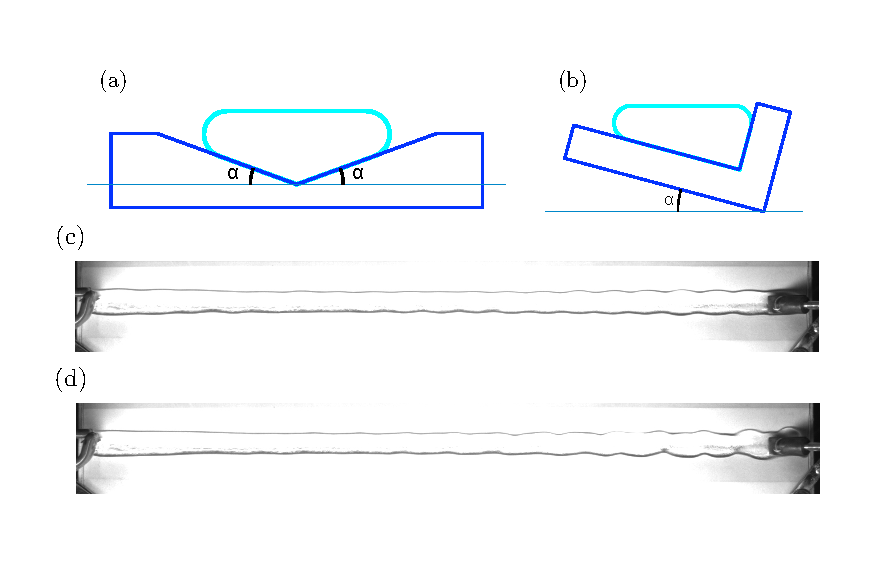
\includegraphics[width=1\textwidth]{./figures/Leidenfrost/modespropagation}
    % \caption{(a) Substrat en V. (b) Substrat en L. (c) Exemple de mode variqueux. (d) Exemple de mode sinueux.}
    % \label{fig:Leidenphoto}
% \end{figure}
% 

% \subsection{Exercices}
% \begin{Exercice}{Exercice : deuxième année PC}
%   On peut en exercice proposer une modélisation plus simple en prenant un écoulement de Marangoni purement radial. Avec un gradient de tension de surface modélisé par une plaque qui entraîne le liquide à la surface à une vitesse constante: diffusion de la quantité de mouvement suivant la direction verticale, analogie avec l'écoulement de Couette.
% \end{Exercice}

% \begin{Exercice}{Exercice : Deuxième année PC}
% 	On peut proposer un exercice équivalent pour l'équation de la chaleur mais pour un transport de particules suivant la direction radiale à la surface de l'eau par exemple.
% \end{Exercice}

% \begin{Exercice}{Exercice: Modélisation de la croissance du tourbillon par conservation de la masse}
%   \begin{enumerate}
%     \item Vecteur tourbillon;
%     \item Conservation du moment angulaire, bilan dans un volume de contrôle;
%     \item Conservation de la masse;
%    \item vecteur densité de flux de particules;
% 		\item Bilan de quantité de matière entrant dans un volume de contrôle;
% 		\item échelle caractéristique de diffusion.
%     \item $r\propto\sqrt{t}$
%   \end{enumerate}
% \end{Exercice}



% % 
% % 
% \begin{Programme}{BO: Deuxième année PC}
%   On peut intégrer ce type d'étude dans le programme de deuxième année de CPGE PC autour des notions suivantes:
% 	\begin{enumerate}
% 		\item Propagation d'ondes.
% 		\item élasticité, module d'Young de la glace
% 		\item relation de dispersion
% 		\item fonte des glaces
% 	\end{enumerate}
% \end{Programme}





% \section{Conclusion}
% \cleardoublepage
% \phantomsection
% \addcontentsline{toc}{chapter}{Bibliographie}
% %%% use of BiBTeX:
% \bibliographystyle{./bib/thesefr-href}
% \bibliography{MaTheseBiblio.bib}
% \cleardoublepage

\end{document}
% 
%
% FIN DU DOCUMENT
%
% 